\documentclass[
	12pt,				% tamanho da fonte
	openright,			% capítulos começam em pág ímpar
	oneside,			% para impressão em recto e verso.
	a4paper,			% tamanho do papel. 
	english,			% idioma adicional para hifenização
	brazil				% o último idioma é o principal do documento
	]{abntex2}

\usepackage{multirow}
\usepackage{multicol}
\usepackage{lmodern}			% Usa a fonte Latin Modern			
\usepackage[T1]{fontenc}		% Selecao de codigos de fonte.
\usepackage[utf8]{inputenc}		% Codificação do documento
\usepackage{indentfirst}		% Indenta o primeiro parágrafo 
\usepackage{color}				% Controle das cores
\usepackage{graphicx}			% Inclusão de gráficos
 			% para melhorias de justificação
\usepackage{mathrsfs,amsmath}   % Usado para criar subequações
\usepackage{listings}           % Used to write code
\usepackage{color}
\usepackage[ruled,vlined]{algorithm2e}  % Used to pseudo code

\usepackage{pdfpages}

\usepackage[brazilian,hyperpageref]{backref}
\usepackage[alf]{abntex2cite}	% Citações padrão ABNT

\renewcommand{\sin}{sen}

\renewcommand{\backrefpagesname}{Citado na(s) página(s):~}
\renewcommand{\backref}{}
\renewcommand*{\backrefalt}[4]{
	\ifcase #1 %
		Nenhuma citação no texto.%
	\or
		Citado na página #2.%
	\else
		Citado #1 vezes nas páginas #2.% 
	\fi}%

\titulo{Construção de modelos baseados na análise de velocidade de dados sísmicos da margem sudoeste da Inglaterra: uma comparação de dados empilhados}
\autor{Paulo Henrique Bastos Alves}
\local{Niterói - RJ}
\data{2021}
\orientador{Luiz Alberto Santos}
\coorientador{Marco Antonio Cetale Santos}
\tipotrabalho{Trabalho de conclusão de curso}
% O preambulo deve conter o tipo do trabalho, o objetivo, 
% o nome da instituição e a área de concentração 
\preambulo{Monografia apresentada à Universidade Federal Fluminense como requisito parcial do Curso de Graduação em Geofísica para a obtenção do título de Bacharel em Geofísica.}

\instituicao{Universidade Federal Fluminense}
\tipotrabalho{Monografia}

% alterando o aspecto da cor azul
\definecolor{blue}{RGB}{41,5,195}

% informações do PDF
\makeatletter
\hypersetup{
		pdftitle={\@title}, 
		pdfauthor={\@author},
    	pdfsubject={\imprimirpreambulo},
	    pdfcreator={LaTeX with abnTeX2},
		pdfkeywords={abnt}{latex}{abntex}{abntex2}{trabalho acadêmico}, 
		colorlinks=true,       		% false: boxed links; true:
    	linkcolor=black,          	% color of internal links
    	citecolor=black,      		% color of links to bibliography
    	filecolor=black,     		% color of file links
		urlcolor=black,
		bookmarksdepth=4
}
\makeatother

\makeatletter
\setlength{\@fptop}{5pt}
\makeatother

\newcommand{\quadroname}{Quadro}
\newcommand{\listofquadrosname}{Lista de quadros}

\newfloat[chapter]{quadro}{loq}{\quadroname}
\newlistof{listofquadros}{loq}{\listofquadrosname}
\newlistentry{quadro}{loq}{0}

% configurações para atender às regras da ABNT
\setfloatadjustment{quadro}{\centering}
\counterwithout{quadro}{chapter}
\renewcommand{\cftquadroname}{\quadroname\space} 
\renewcommand*{\cftquadroaftersnum}{\hfill--\hfill}

\setfloatlocations{quadro}{hbtp} % Ver https://github.com/abntex/abntex2/issues/176

% O tamanho do parágrafo é dado por:
\setlength{\parindent}{1.3cm}

% Controle do espaçamento entre um parágrafo e outro:
\setlength{\parskip}{0.2cm}  % tente também \onelineskip

\makeindex

\renewcommand{\imprimircapa}
{
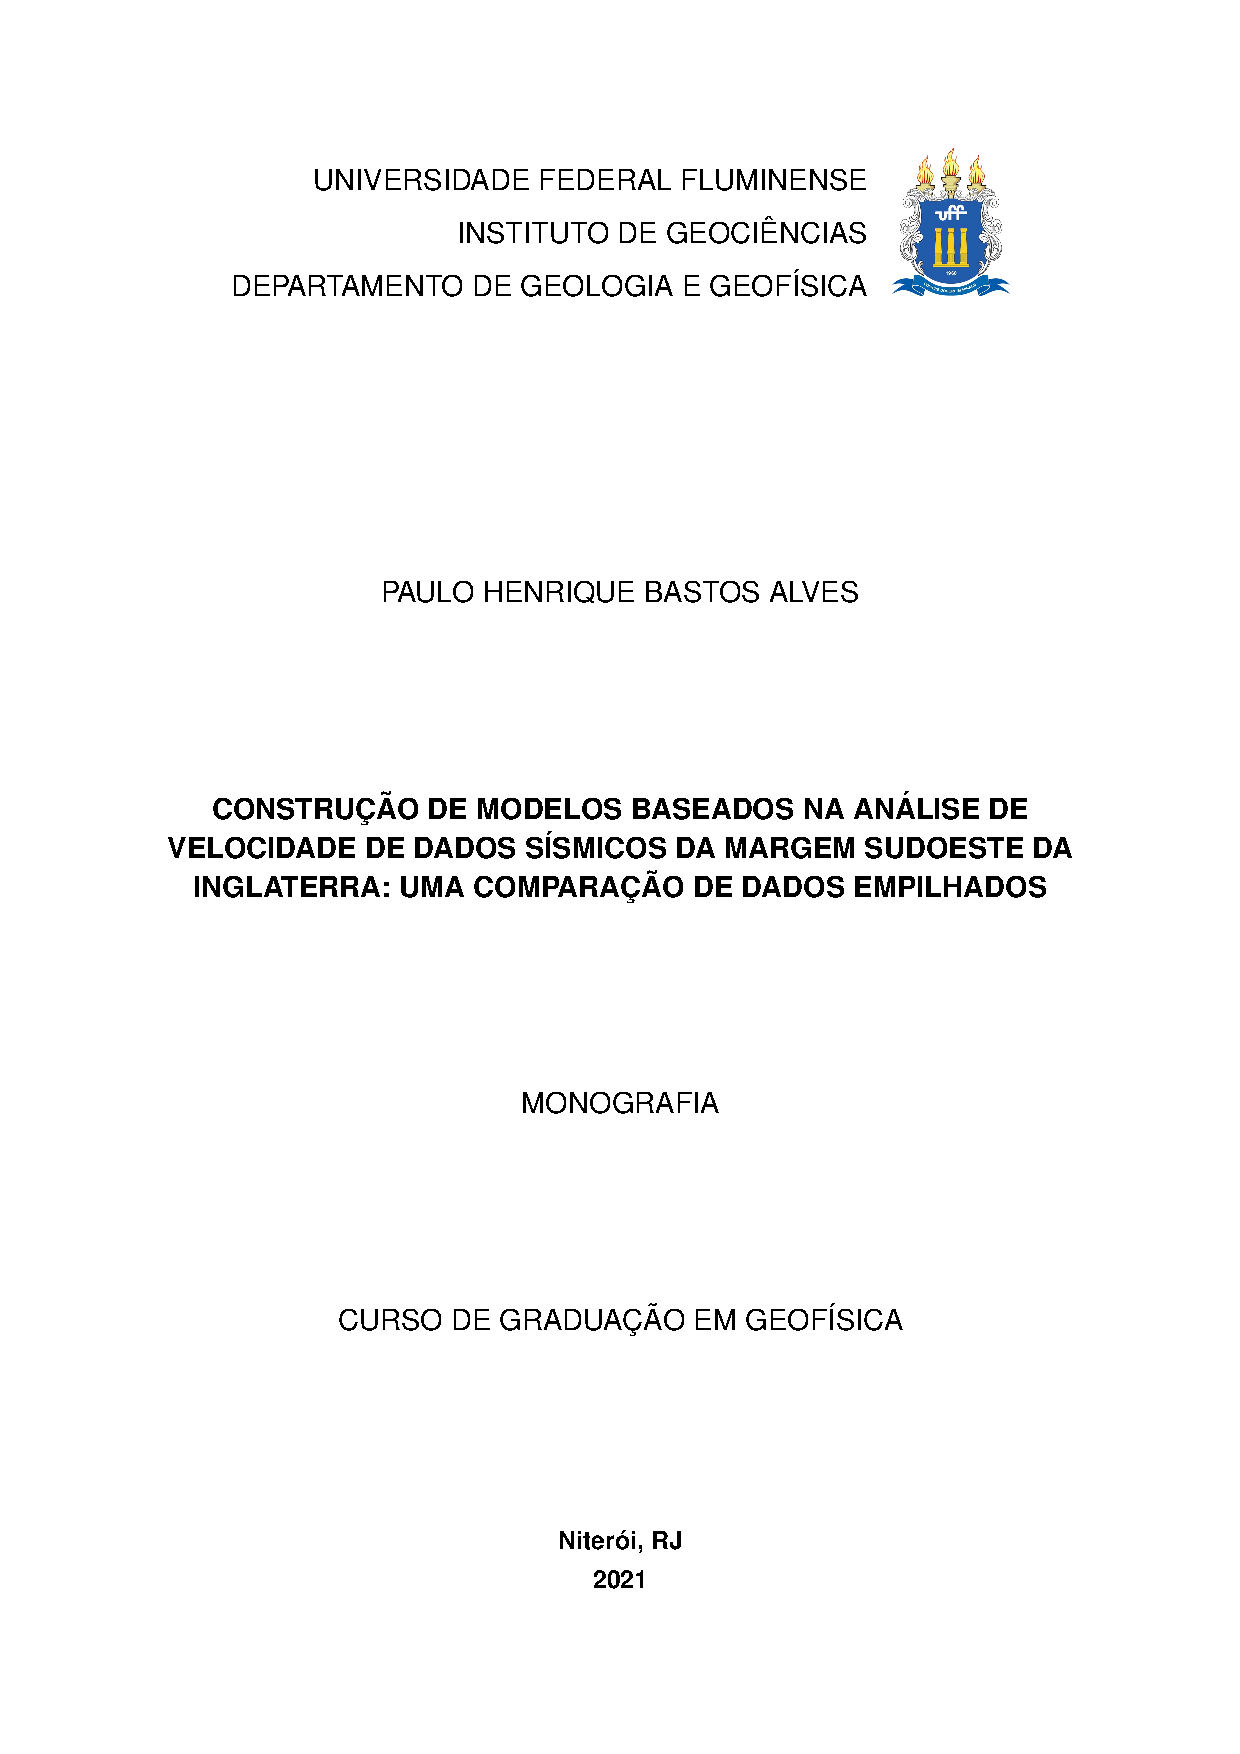
\includepdf{capa.pdf}
}

\newcommand{\fonteLocalData}{\fontsize{12}{14}\selectfont}
\renewcommand{\imprimirfolhaderosto}
{
	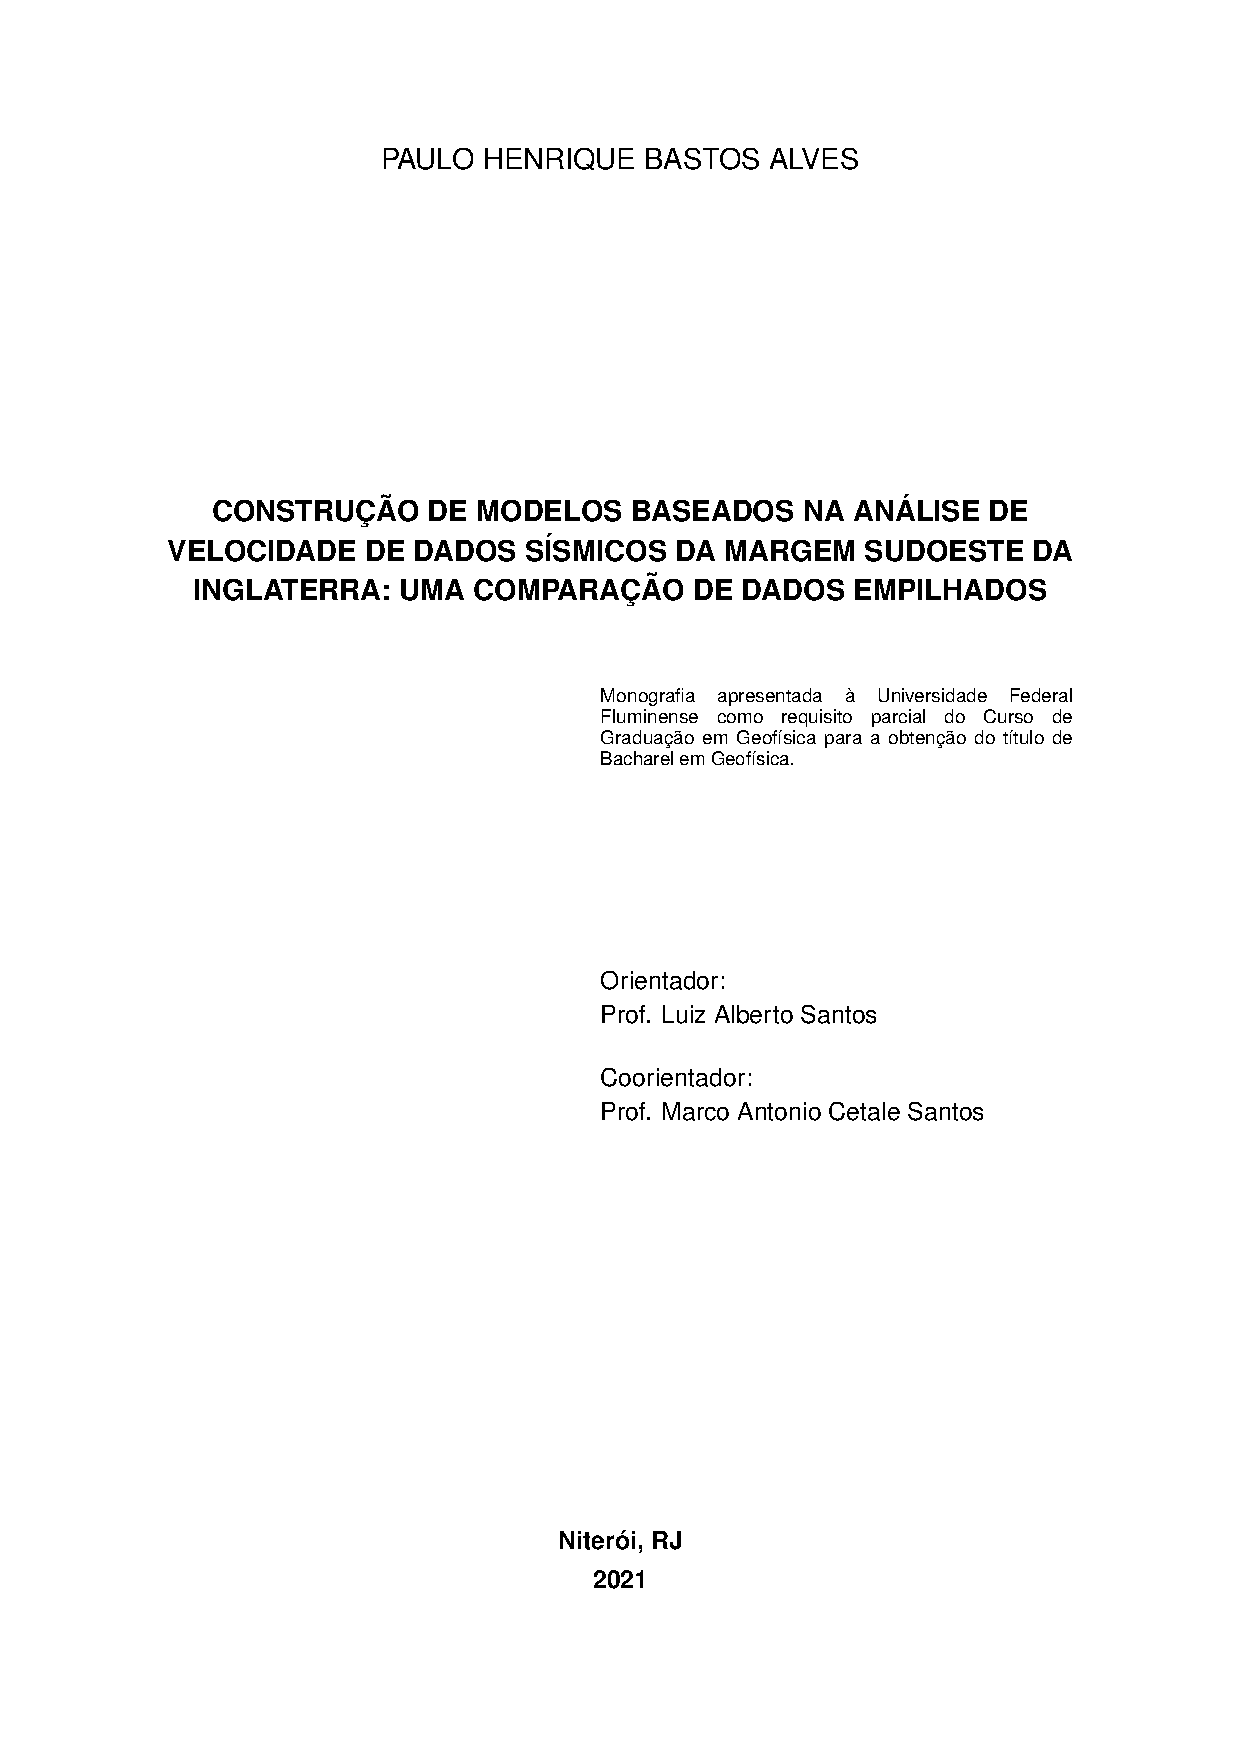
\includepdf{folhaRosto.pdf}	
}

% Início do documento 
\begin{document}

\selectlanguage{brazil}

\frenchspacing 

\imprimircapa

\imprimirfolhaderosto

% Ficha cartalográfica
\begin{fichacatalografica}
    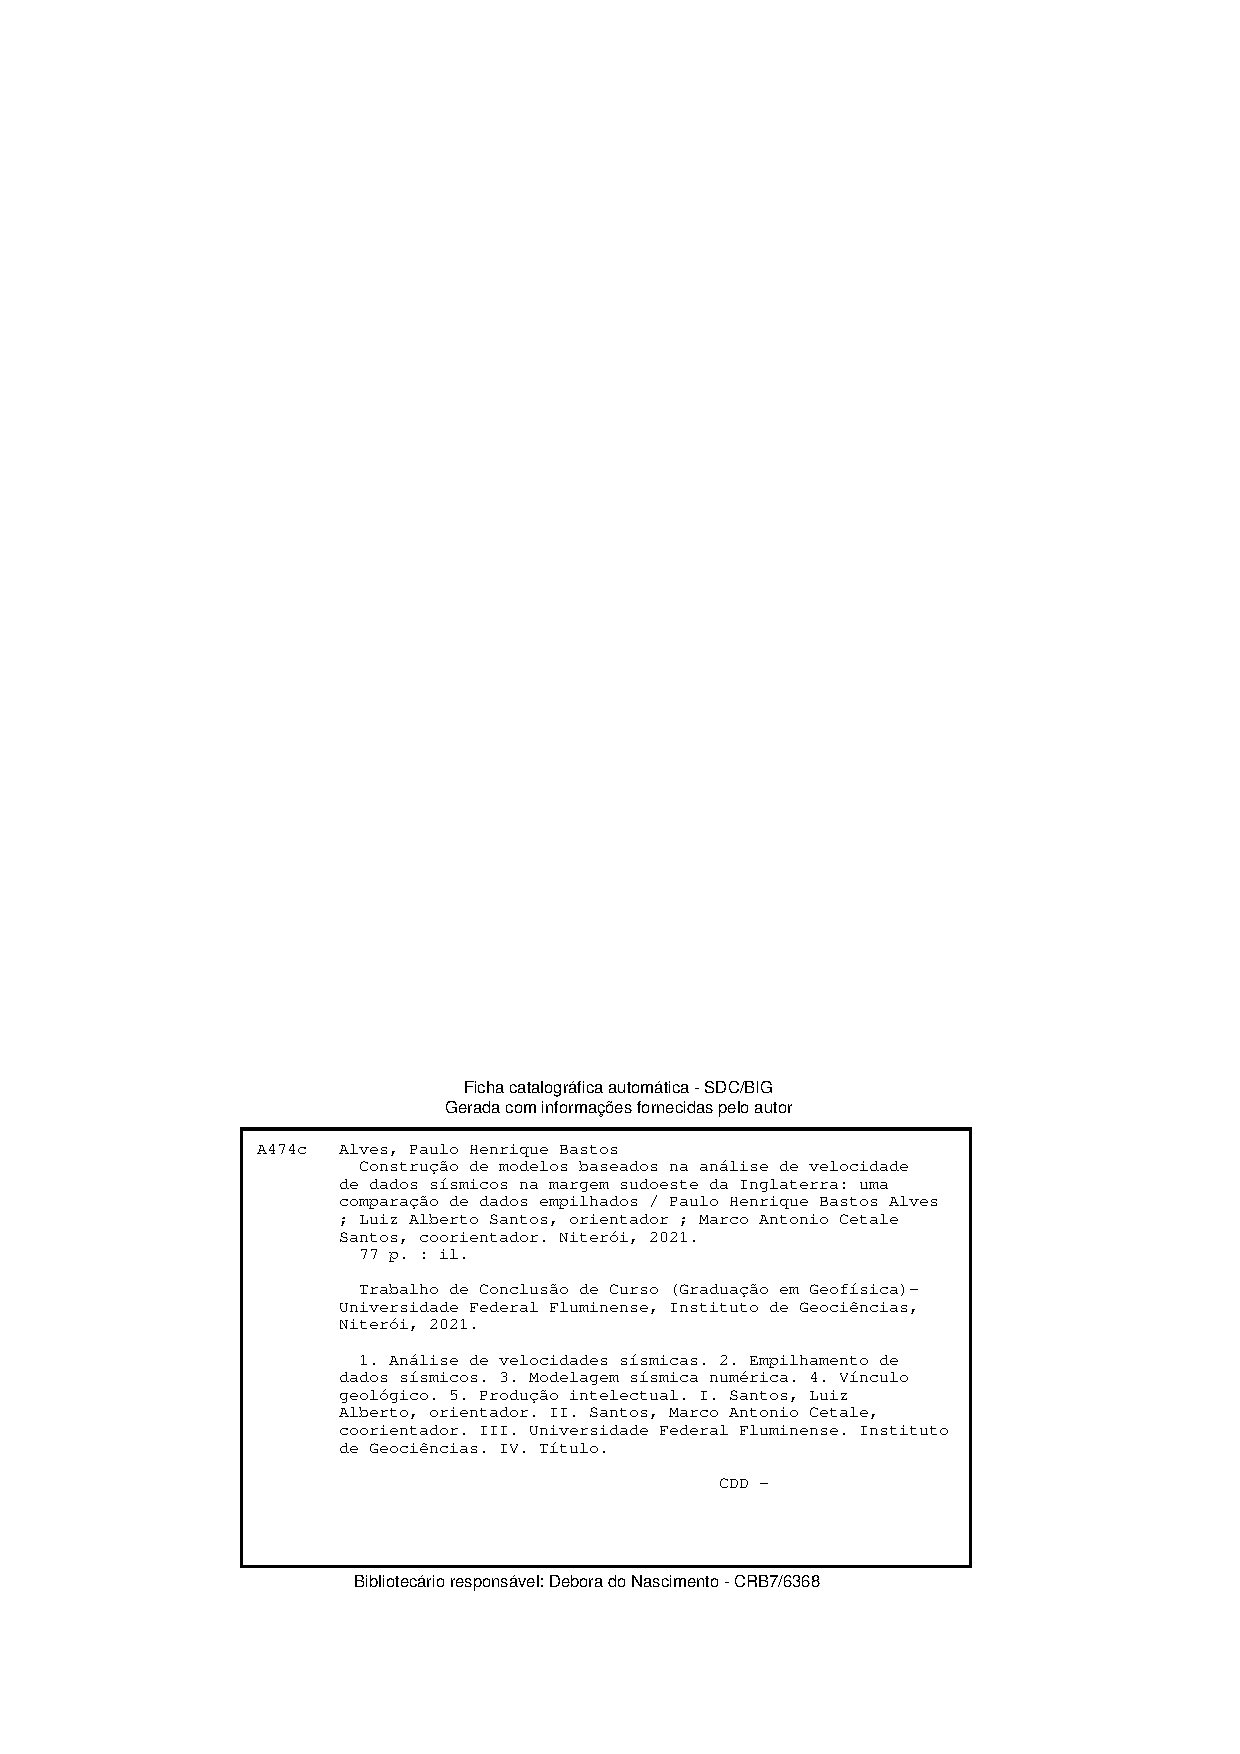
\includepdf{ficha.pdf}
\end{fichacatalografica}

% Folha de aprovação
\begin{folhadeaprovacao}
	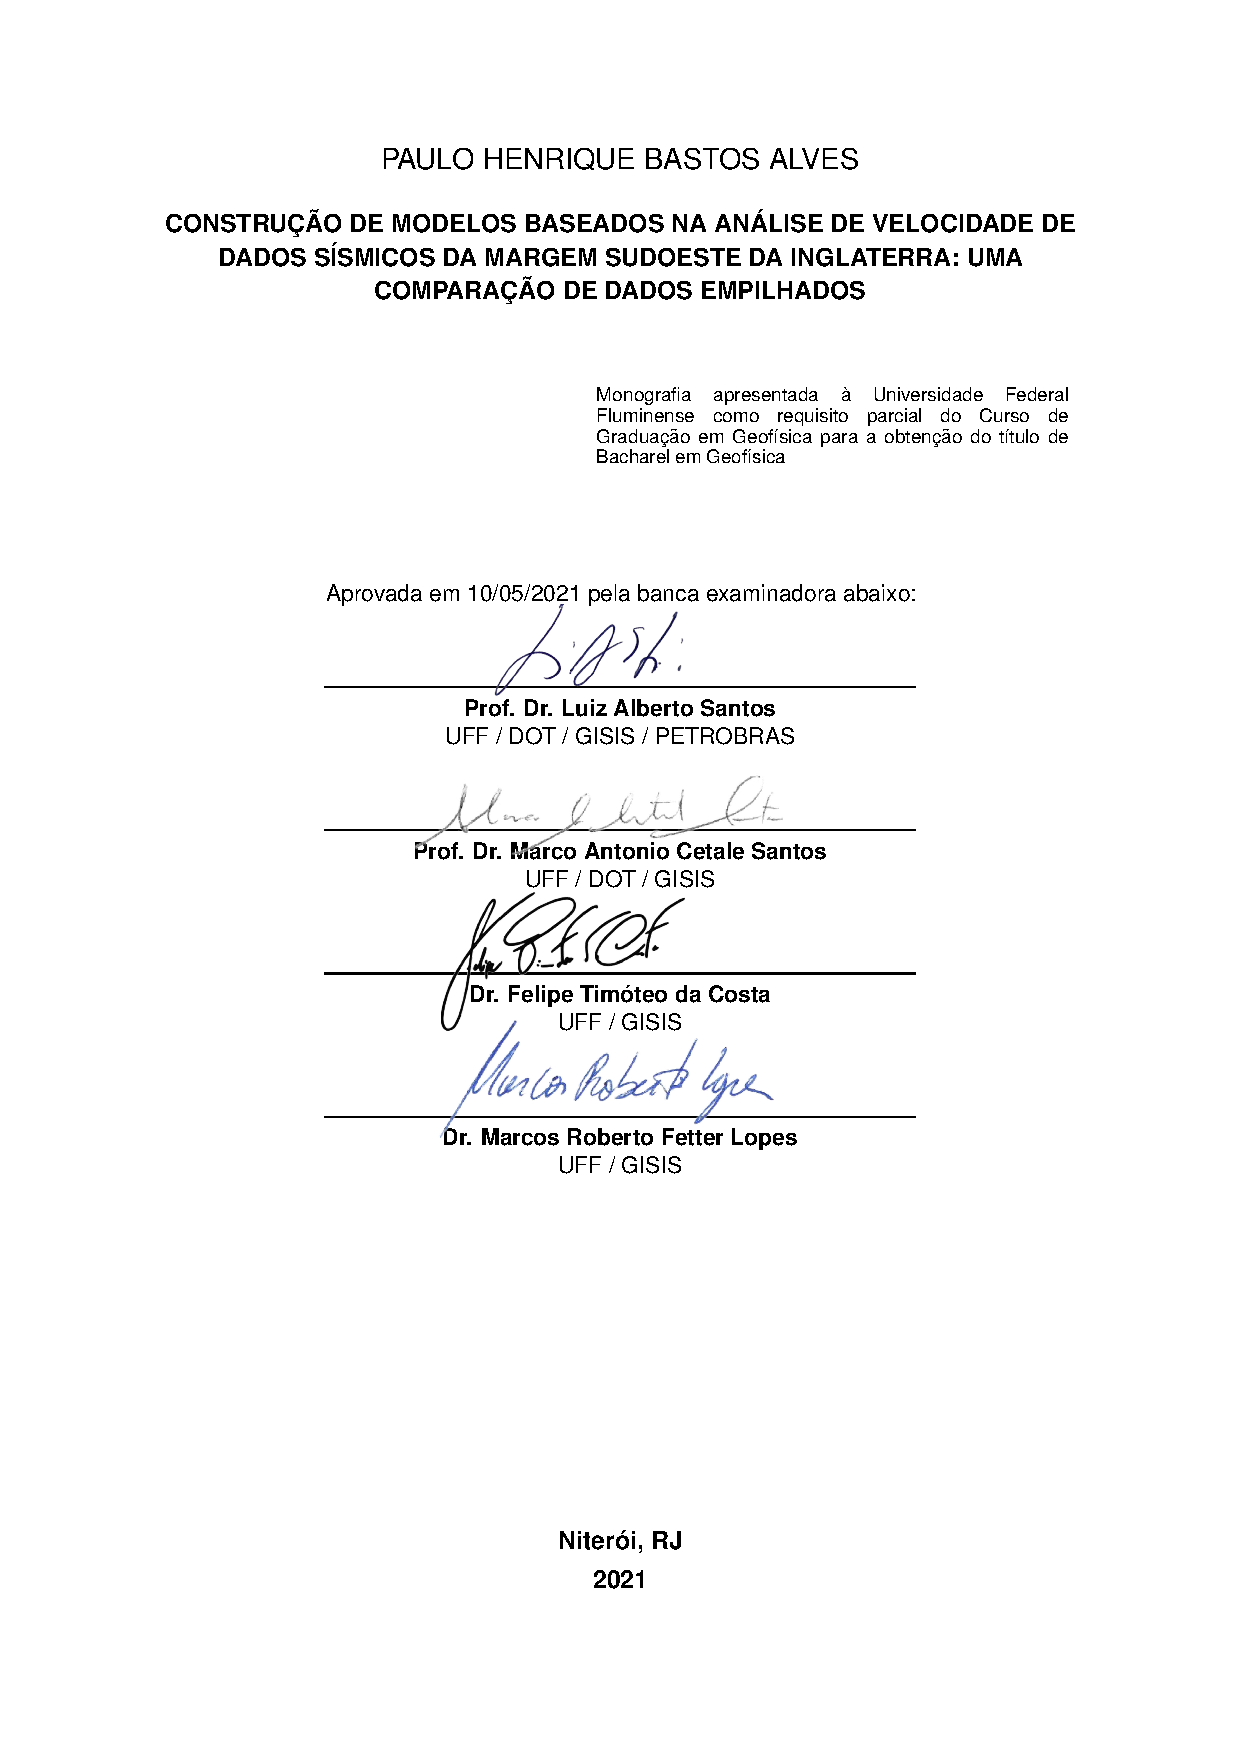
\includepdf{folhaAprovacao.pdf}  
\end{folhadeaprovacao}

% Dedicatória
\begin{dedicatoria}
	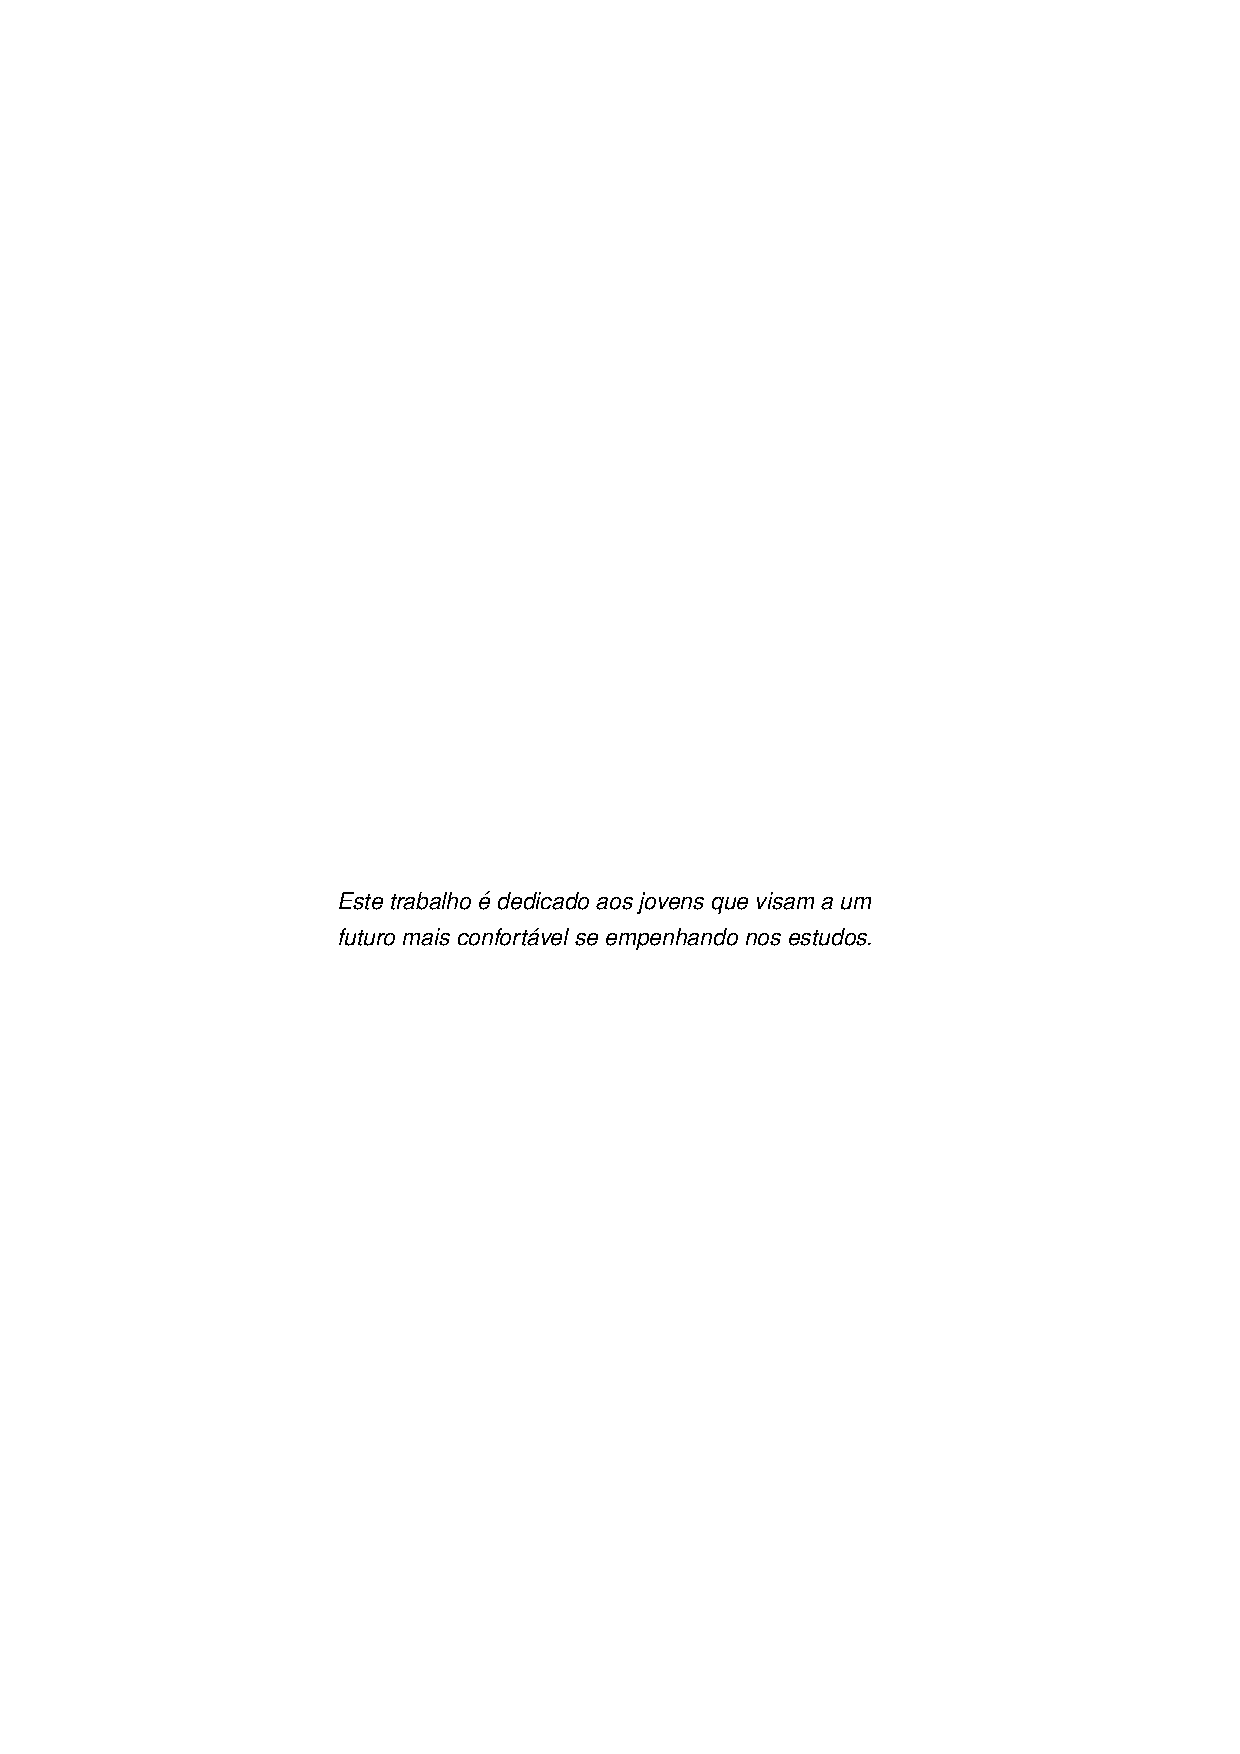
\includepdf{dedicatoria.pdf}
\end{dedicatoria}

% Agradecimentos
\begin{agradecimentos}
	
	Gostaria de agradecer à minha família, que desde sempre tive apoio quando se tratava de estudar. Um agradecimento especial à minha mãe, que sacrificou a maior parte da vida, trabalhando sem cessar, para me manter estudando sem muitas complicações, me proporcionando todo o subsídio para direcionar os meus empenhos nos estudos.
	
	Eu agradeço às instituições de ensino público do Estado do Rio de Janeiro, onde sempre estudei e que me fizeram observar o valor do conhecimento. Outra questão, agradeço às bem preparadas refeições, cedidas com carinho pelas instituições públicas, fizeram toda a diferença na minha formação como pessoa.    
	
	Um agradecimento especial à Universidade Federal Fluminense, que ingressei por meio de políticas afirmativas. Obrigado pelos serviços, pelas iniciativas sociais e pelas oportunidades de crescimento profissional (Horizonte Soluções Geofísicas) e acadêmico (monitoria de Processamento Digital de Sinais). 

	Obrigado aos meus orientadores, Luiz Alberto Santos e Marco Cetale, pelas oportunidades de aprender e pelas orientações cirúrgicas. Por consequência das nossas conversas constantes às quartas, este trabalho foi concluído com sucesso.   
	
	Gostaria de agradecer também, ao projeto de pesquisa do campo de Búzios, vinculado à Petrobras, que participei durante mais de dois anos da minha formação. Os meus conhecimentos de programação, método sísmico e propagação de ondas se devem à minha participação nesse projeto. Assim, eu pude entrar em contato com pessoas que eu jamais conheceria, somente participando das matérias da graduação em geofísica.  
	
	Um grande obrigado ao grupo de imageamento sísmico e inversão sísmica, que me proporcionou experiências incríveis fora e dentro do escritório. Eu pude participar de alguns trabalhos de campo utilizando o método sísmico terrestre, com o grupo. Eles me fizeram valorizar o dado adquirido em campo, pois o processo de aquisição sísmica é árduo. Agradeço às pessoas do grupo também, por serem sempre solícitas e dispostas quando o assunto é resolver problemas e sanar dúvidas. 
	
	Agradeço aos amigos que criei na jornada de universitário, me fizeram manter a saúde mental durante os desesperos das provas. Aos meus amigos do instituto geociências, veteranos e calouros, do basquete universitário, da dança UFF e os muito especiais dos grupos \textit{Testemunhas do 302} e \textit{Tralhas em latim on-line}, gratidão pelas conversas e momentos de bem estar.  
	 
\end{agradecimentos}

% Epígrafe
\begin{epigrafe}
	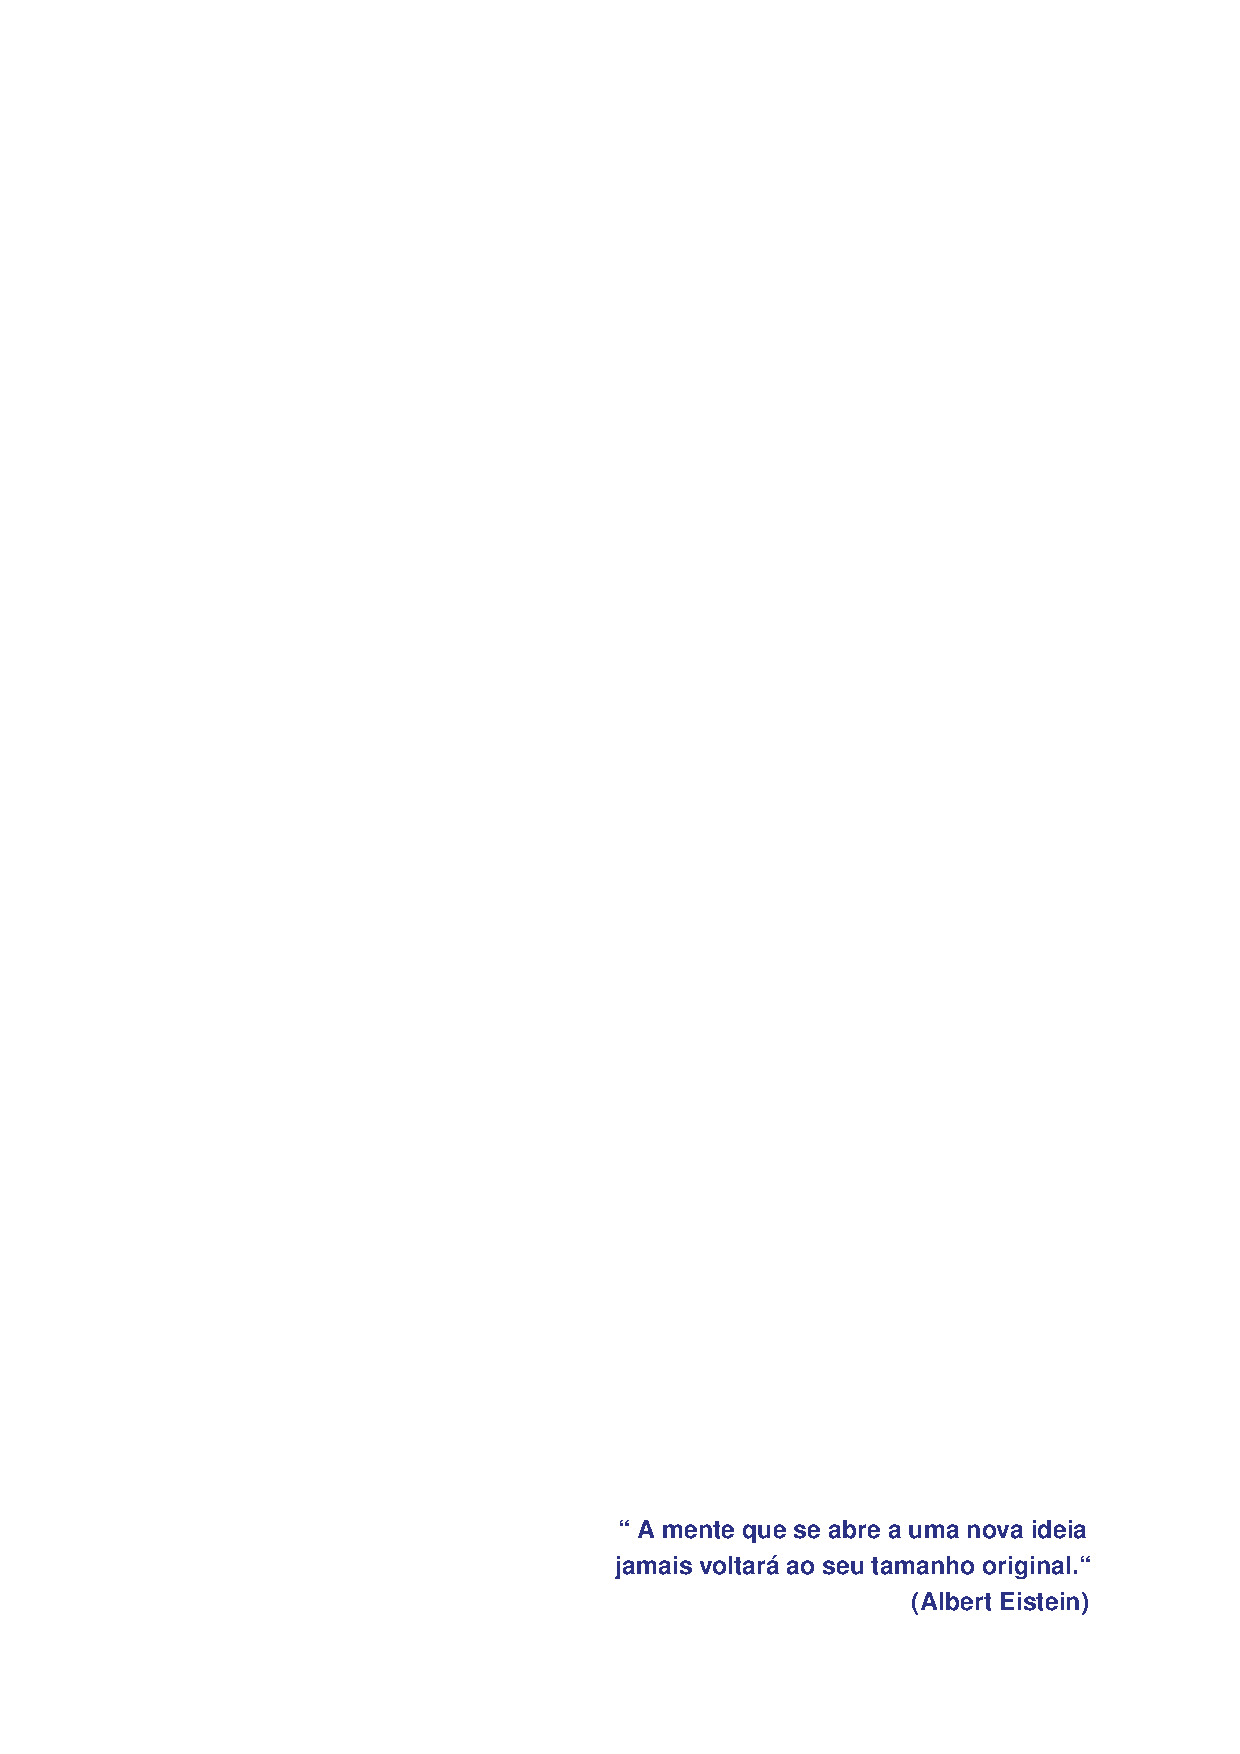
\includepdf{epigrafe.pdf}
\end{epigrafe}

% Resumo em português
\setlength{\absparsep}{18pt} % ajusta o espaçamento dos parágrafos do resumo
    \begin{resumo}		

		A partir de um pacote de dados sísmicos pré-empilhados adquiridos no mar Celta, margem sudoeste da Inglaterra, recuperamos o campo de velocidades da onda compressional $v_p$. O método de estimativa utilizado foi a análise de velocidades, que tenta horizontalizar as hipérboles de reflexão em sismogramas de ponto médio comum. Em seguida os dados sísmicos reais foram processados e migrados em tempo e, nesta seção foram mapeados os horizontes com maior continuidade lateral. Utilizando as velocidades estimadas a partir do dado real, foi criado um modelo inicial de propriedades elásticas com $v_p$, $v_s$ (velocidade da onda cisalhante) e $\rho$ (densidade). Sobre os modelos de propriedades realiza-se uma modelagem sísmica com formulação elástica isotrópica e od dados gerados sinteticamente foram processados da mesma forma que os dados reais. Destes foram mapeados os mesmos horizontes observados nos dados reais. A partir das diferenças entre os horizontes obtidos, o modelo de propriedades elásticas é atualizado levando-se em conta a geologia e informações de perfis de poços. Assim foi possível criar um vínculo geológico nas propriedades gerando-se um novo modelo. Novos pacotes de dados sísmicos sintéticos foram gerados utilizando o modelo de propriedades atualizado e baseado na geologia específica da região. A comparação pós-empilhamento dos três pacotes de dados sísmicos, real, primeiro sintético e sintético corrigido foi feita. Observou-se uma melhora expressiva na correspondência dos horizontes reais e aqueles obtidos com o modelo corrigido.

    \vspace{\onelineskip}
    \newline 
    \textbf{Palavras-chave}: Análise de velocidades. Empilhamento de dados sísmicos. Modelagem sísmica. Vínculo geológico.
\end{resumo}

% Resumo em inglês
\begin{resumo}[Abstract]
    \begin{otherlanguage*}{english}

	From a pre-stacked seismic data package acquired in the Celtic Sea, southwest of England, we recovered the velocity field of the compressional wave $v_p$. The estimation method used was the velocity analysis, which tries to horizontalize the reflection hyperbolas in common mid point seismograms. Then the real seismic data were processed and migrated in time and, in this section, the horizons with greater lateral continuity were mapped. Using the estimated velocities from of the real data, an initial elastic properties model with $v_p$, $v_s$ (shear wave velocity) and $\rho$ (density) was generated. Seismic modeling is carried out on it with isotropic elastic formulation and processed in the same way as the real data. Of these sinthetic data were mapped the same horizons seen in the real seismic section. From the differences between the horizons obtained, the model of elastic properties is updated taking into account the geology and well profile information. Thus, it was possible to create a geological link in the properties generating a new model. New synthetic seismic data packages were generated using the updated property model and based on geology specific to the region. The post-stack comparison of the three seismic data packages, real, first synthetic and corrected synthetic was made. There was a significant improvement in the correspondence of the real horizons and those obtained with the corrected model.

    \vspace{\onelineskip}
    \newline
    \textbf{Keywords}: Velocity analysis. Seismic data stacking. Seismic modeling. Geological link.
    \end{otherlanguage*}
\end{resumo}

% Inserir lista de ilustrações
\pdfbookmark[0]{\listfigurename}{lof}
\listoffigures*
\cleardoublepage

% Inserir lista de quadros
%\pdfbookmark[0]{\listofquadrosname}{loq}
%\listofquadros*
%\cleardoublepage

% Inserir lista de tabelas
%\pdfbookmark[0]{\listtablename}{lot}
%\listoftables*
%\cleardoublepage

% Inserir lista de abreviaturas e siglas
\begin{siglas}
  \item[CMP] \textit{Commom Mid Point} 
  \item[FFT] \textit{Fast Fourier Transform}
  \item[GISIS] Grupo de Imageamento Sísmico e Inversão Sísmica
  \item[IFFT] \textit{Inverse Fast Fourier Transform}
  \item[INT] Intervalar
  \item[IVA] \textit{Iteractive Velocity Analysis}
  \item[NMO] \textit{Normal Move Out}
  \item[OBC] \textit{Ocean Bottom Cables}
  \item[OBN] \textit{Ocean Bottom Nodes}
  \item[RMS] \textit{Root Mean Square}
  \item[SU] \textit{Seismic Unix}  
  \item[UFF] Universidade Federal Fluminense
\end{siglas}

% Inserir lista de símbolos
\begin{simbolos}
  \item[$ \theta $] Ângulo qualquer 
  \item[$ \mu $] Constante de cisalhamento
  \item[$ \lambda $] Constante de compressibilidade 
  \item[$ \varepsilon $] Deformação
  \item[$ \rho $] Densidade
  \item[$ \partial $] Derivada parcial
  \item[$ \in $] Pertence
  \item[$ \nu $] Razão de Poisson
  \item[$ \sigma $] Tensão
  \item[$ \Delta $] Variação
  \item[$ v_s $] Velocidade da onda cisalhante
  \item[$ v_p $] Velocidade da onda compressional
\end{simbolos}

% Inserir o sumario
\pdfbookmark[0]{\contentsname}{toc}
\tableofcontents*
\cleardoublepage

\textual

\chapter{Introdução}

	A geofísica é uma ciência que engloba múltiplas áreas do conhecimento, tal como física, matemática, geologia e programação de computadores. Os trabalhos de \citeonline{telford1990applied}, \citeonline{reynolds2011introduction} e \citeonline{kearey}, mostram a abrangência da geofísica descrevendo a maioria dos métodos e técnicas para coletar dados da natureza. Então, a geofísica se baseia na coleta de dados, onde instrumentos específicos medem as propriedades físicas que existem no meio de maneira passiva ou ativa, onde equipamentos perturbam o meio para que sensores possam quantificar tais perturbações. A partir dos dados adquiridos, uma série de processos são realizados para que a representação do meio, ou do fenômeno, seja a mais fidedigna possível.      

	O método sísmico é utilizado neste trabalho, sendo o seu funcionamento baseado na injeção artificial de ondas mecânicas no meio, para que sensores possam registrar as amplitudes das perturbações na superfície de acordo com o tempo de trânsito. Os estudos de \citeonline{aki2002quantitative} e \citeonline{carcione2007wave}, descrevem detalhadamente a parte ondulatória do fenômeno sísmico. Os trabalhos de \citeonline{robinson2000geophysical} e \citeonline{rosa2010analise}, mostram a base matemática para lidar com os sinais sísmicos em tempo. E os autores \citeonline{sheriff1995exploration}, \citeonline{yilmaz2001seismic} e \citeonline{alsadi2017seismic}, abordam sobre os processos realizados no sinal sísmico de maneira prática, em relação às aquisições de dados reais.
	
	A estimativa das propriedades físicas das rochas em uma região desconhecida em si já é motivador, porém o que motivou o trabalho foi aplicar técnicas de processamento e imageamento sísmico utilizando desenvolvimento de algoritmos próprios. Então, os desafios da adaptação do modelo de propriedades e uma simulação de alta performance do campo de onda completo foram a base motivacional do trabalho. Outro motivo, foi o entendimento completo da geometria de uma aquisição sísmica convencional em duas dimensões. Apesar das aquisições sísmicas se apresentarem mais complexas atualmente, o conhecimento base facilita o entendimento das configurações atuais. Os processos de estimativa de velocidade da onda compressional são sempre desafiadores, porém o conhecimento da geologia aliado aos métodos de estimativa fizeram a completa diferença no resultado final.      
	   
	O dado sísmico foi adquirido na margem sudoeste da Inglaterra, mais precisamente no mar Celta, um pouco acima da desembocadura do canal de Bristol. A razão de se estar estudando a área seria pelo fácil acesso aos dados da região, disponibilizados pelo Prof. Dr. Luiz Alberto Santos, orientador deste estudo, adquiridos pela \textit{Oil and Gas Authority} do Reino Unido, para agregar os trabalhos de graduação e pós-graduação de seus orientandos. O dado sísmico escolhido uniu os aspectos de qualidade e armazenamento compacto.    
	
	O objetivo do trabalho é construir um modelo de velocidade da onda compressional que melhor representa a região de aquisição na margem sudoeste da Inglaterra, utilizando o dado real, gerando modelos através da análise de velocidades e comparando seções empilhadas sintéticas com a seção real. As seções sintéticas são geradas a partir de uma simulação sísmica aproximada para meios elásticos isotrópicos, a comparação é feita através da interpretação dos horizontes das seções e as diferenças são averiguadas a partir do erro absoluto entre as posições em tempo dos horizontes.      	
	
	Este trabalho apresentará quatro capítulos, sendo o primeiro deles chamado de fundamentação teórica. Nele, toda a teoria necessária para a reprodução deste trabalho será apresentada, sendo que a parte da área de estudo, localiza e expõe os principais aspectos geológicos da região. A parte do processamento sísmico, aborda as principais modificações que poderiam ser feitas no dado sísmico e apresenta o método de estimativa das velocidades da onda compressional. E a parte da modelagem sísmica para meios elásticos isotrópicos descreve as ferramentas necessárias para realizar uma simulação sísmica computacional.
	
	O capítulo de materiais e métodos aborda as metodologias utilizadas para gerar os modelos a partir do dado sísmico. Primeiro são descritas as características do dado, mostrando as distribuições espaciais da aquisição e as componentes de cada traço sísmico. Em seguida, a construção do modelo de velocidades é apresentada, detalhando cada etapa realizada até a construção do modelo de velocidades da onda compressional. Na parte do empilhamento do dado real é apresentada a seção resultante do processamento sísmico em coordenadas genéricas. A seção voltada para a construção dos modelos de propriedades elásticas prepara os modelos iniciais, a fim de serem utilizados no processo apresentado posteriormente. Na modelagem sísmica descrevemos todas as etapas realizadas na simulação sísmica computacional. Na parte do pré-condicionamento para o empilhamento do dado sintético são abordadas as modificações do dado sintético realizadas anteriormente ao processo de empilhamento, visando à melhorias na seção final.       	

	O capítulo de resultados e discussões descreve os resultados, aborda sobre a alternativa para solucionar o problema de comparação e expõe as análises resultantes geradas a partir dos resultados. Uma breve discussão geológica, baseada em perfis de poços, é feita para analisar as causas dos problemas de comparação entre as seções empilhadas real e sintética.	

	Por fim, o capítulo de conclusão sintetiza o trabalho apresentando as vantagens e desvantagens dos processos utilizados. Os pontos negativos se observam a partir do método de estimativa não conseguindo gerar um modelo que representasse o sinal empilhado em tempo. Já os pontos positivos, são apresentados a partir da aplicação de um gradiente de velocidade decrescente com a profundidade no modelo de acordo com a geologia, onde houve melhorias na comparação entre horizontes real e sintético. 

\chapter{Fundamentação teórica}

    Este capítulo tem como objetivo descrever a teoria necessária para se alcançar o resultado final proposto neste trabalho. A abordagem se mostrará simples, de modo a estimular um maior entendimento prático sobre os assuntos relatados, não negligenciando as literaturas que abordam profundamente os aspectos teóricos relacionadas aos temas.   

\section{Área de estudo}

	Nesta seção a região de interesse, margem sudoeste da Inglaterra, será apresentada com o objetivo de observar as principais características geométricas e litológicas de subsuperfície próximas ao local de aquisição do dado sísmico que foi utilizado neste trabalho. A Figura \ref{pontosTiro}, mapeada com a linguagem de programação python utilizando a biblioteca Cartopy, mostra explicitamente a localização onde os dados foram adquiridos, sendo ilustrados os pontos de disparo sísmico representando toda a aquisição. 

    \begin{figure}[htp!]
		\centering
		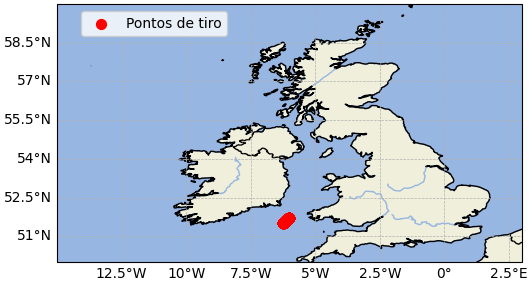
\includegraphics[width=13cm,height=7.5cm]{../imagens/area_de_estudo.png}
		\caption{Margem sudoeste da Inglaterra mostrando a localização dos disparos sísmicos contidos na aquisição do dado sísmico utilizado neste trabalho.}
		\label{pontosTiro}
	\end{figure}

	A profundidade do assoalho oceânico da região não ultrapassa os 200 metros, contendo uma média entre 100 e 150 metros de profundidade \cite{hamilton1979geology}, como mostrado na figura \ref{batimetria}. Essa característica será marcada fortemente no dado sísmico e o conhecimento regional da topografia de fundo marinho será crucial para construir um bom modelo de propriedades utilizando a aproximação para meios elásticos isotrópicos.
	
    \begin{figure}[htp!]
		\centering
		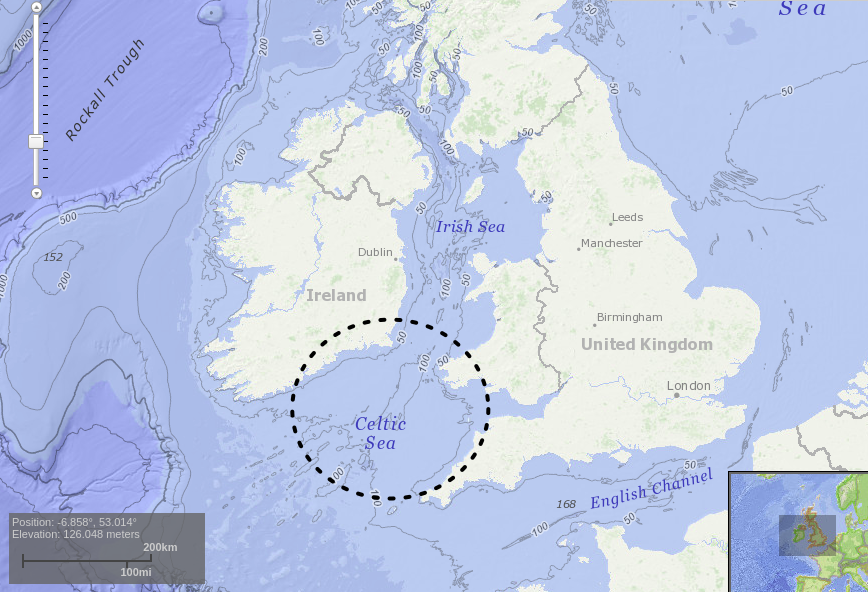
\includegraphics[width=12cm,height=9cm]{../imagens/batimetria.png}
		\caption{Batimetria da região delimitando o local de aquisição \cite{NOAA}.}
		\label{batimetria}
	\end{figure}

	O trabalho pioneiro da região foi de \citeonline{dangeard1923quelques}, com a construção de mapas cartográficos e coleta de amostras geológicas. Em seguida temos a síntese de \citeonline{king1954geological}, que contextualiza uma história geológica para a região do canal Inglês.
	
	Em \citeonline{smith1975structure} se descreve a evolução estrutural e geológica separando as regiões em províncias, cada uma com distintas características. É construído uma tabela estratigráfica relacionando as diferentes províncias e suas respectivas principais litologias. São apresentados também perfis geológicos por todo o canal Inglês evidenciando a localização das litologias e a predominância do direcionamento das falhas.
	
	No trabalho de \citeonline{hamilton1979geology}, a morfologia da região do canal Inglês é enfatizada levando em consideração a litologia. Comenta-se sobre a natureza do fundo marinho mostrando mapas topográficos e discutindo sobre os fluxos sedimentares em diferentes épocas de tempo geológico.
	
	\citeonline{dyment1990deep} mostram uma análise mais crustal e profunda utilizando a ferramenta de gravimetria para averiguar as anomalias de densidade no canal Inglês. E \citeonline{ruffell1995geometry} priorizam a geologia estrutural rasa e destacam o direcionamento das falhas na região, mostrando perfis de poços, detalhando a litologia e classificando as mega sequências sismoestratigráficas através de perfis sísmicos.
	
	O trabalho de \citeonline{glen2005basin} apresenta a geologia estrutural e o lineamento das falhas (Figura \ref{falhas}). Esse trabalho mostra também modelos de inversão de bacia sedimentar formada em regime distensivo, destacando modelos estruturais que originaram a região do canal Inglês. 
	
    \begin{figure}[htp!]
		\centering
		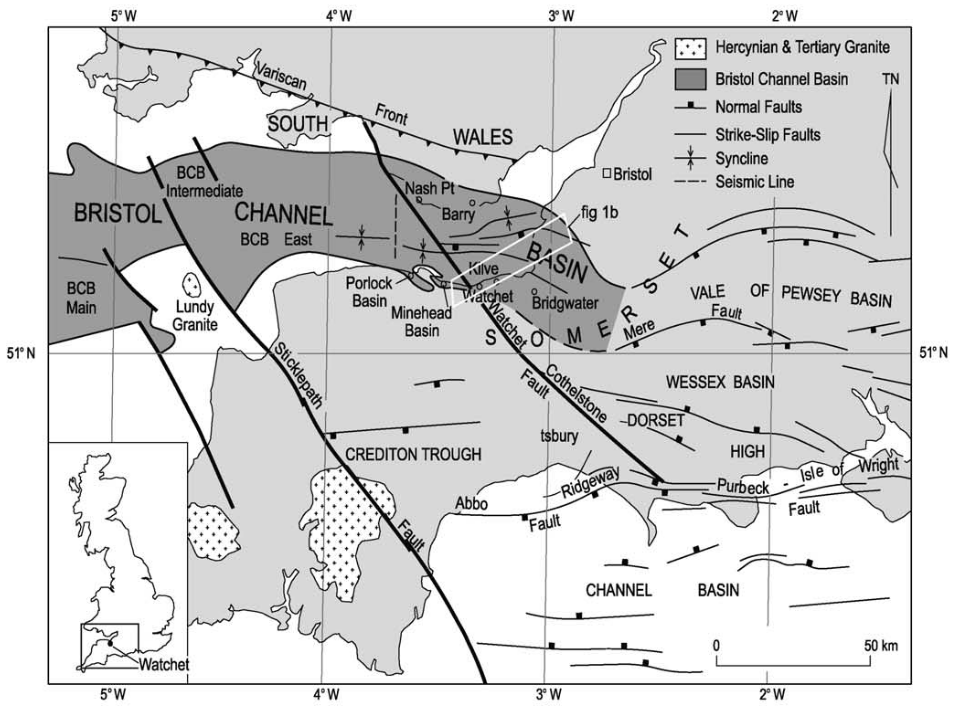
\includegraphics[width=12cm,height=8cm]{../imagens/geologia.png}
		\caption{Estrutura, lineamento e características das falhas próximas da região de interesse, no canal de Bristol. Predominância de falhas normais e lineamentos de falhas transcorrentes \cite{glen2005basin}.}
		\label{falhas}
	\end{figure}

	Embora os estudos dos trabalhos apresentados acima estejam focados no interior do canal de Bristol, pôde-se ter uma ideia sobre o que esperar da geologia de subsuperfície na região onde o dado utilizado foi adquirido. A região é composta majoritariamente de falhas normais com certos lineamentos de falhas transcorrentes (Figura \ref{falhas}). A região de interesse se encontra mais especificamente no mar Celta, à nordeste da região mostrada na figura \ref{falhas}. 

	O real conteúdo coletado nos artigos de referência é a litologia regional (Figura \ref{estratos}). Com isso, as velocidades sísmicas podem ser melhor analisadas no método de estimativa, pois um vínculo com a geologia pode ser criado para embasar a estimativa. A região apresenta rochas carbonáticas rasas (\textit{limestone} e \textit{chalk}) que possuem uma faixa de velocidades alta. Como por exemplo o \textit{limestone} (calcário), que abrange grande parte das cartas estratigráficas da região de interesse, tem uma variação de velocidades sísmicas compressionais de 3000 a 6000 metros por segundo dependendo da profundidade \cite{mavko2020rock}.  

	Sabendo da configuração litológica da região, estabeleceu-se uma base para a estimativa de velocidades sísmicas utilizando o método da análise de velocidades, que será apresentado na seção a seguir.

	\newpage		
    \begin{figure}[htp!]
		\centering
		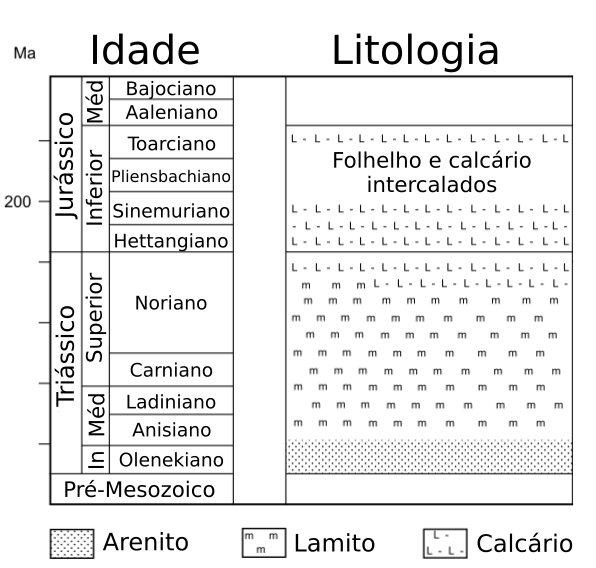
\includegraphics[width=9cm,height=7.2cm]{../imagens/regional.png}
		\caption{Carta estratigráfica regional do canal de Bristol, apresentando os tempos geológicos e as principais litologias presentes na região (adaptado de \citeonline{glen2005basin}).}
		\label{estratos}
	\end{figure}

\section{Processamento sísmico}

    O método sísmico consiste em captar ondas mecânicas, disparadas por fontes artificiais, em sensores posicionados na superfície terrestre ou marítima, no assoalho oceânico e até mesmo dentro de poços perfurados \cite{kearey}. A sísmica de exploração foi projetada para que as ondas mecânicas iluminem um mesmo ponto em subsuperfície o máximo de vezes que a geometria de aquisição permitir. Sendo assim, dezenas de milhares de disparos são realizados para um mesmo grupo de sensores, que se movimentam em um determinado sentido, para o caso de aquisições convencionais bidimensionais \cite{sheriff1995exploration}. Cada sensor registra um traço sísmico na posição em que se encontra, contendo o tempo em que as perturbações no meio, causadas pelas ondas, chegam à posição de um determinado sensor. Sabendo esse processo, cada traço sísmico adquirido é coletado e armazenado em um arquivo específico, contendo todas as informações de posicionamento com base na geometria de aquisição pré-estabelecida \cite{aki2002quantitative}.
    
    O processamento sísmico pode ser usado para transformar amplitudes sísmicas incapazes de representar feições geológicas, em sinais que possivelmente simbolizam a geologia. Esse processo é extremamente amplo e variado, aplicando-se tipos específicos de procedimentos de acordo com o dado ou melhor ainda, utilizando métodos relacionados com a história geológica que formou a subsuperfície da região onde o dado foi adquirido \cite{yilmaz2001seismic}. Então, as técnicas de processamento que serão abordadas neste capítulo tem como objetivo apresentar a teoria das ferramentas utilizadas pelo autor, que posteriormente serão aplicadas ao dado sísmico da margem sudoeste da Inglaterra.   
	
    \subsection*{Ordenação de traços sísmicos}

    Em levantamentos marítimos convencionais, a fonte se localiza próximo da embarcação que traciona um cabo com centenas de receptores. Assim se forma o primeiro tipo de ordenação de traços sísmicos, contendo os receptores na ordem em que receberam o disparo da fonte chamado de domínio do tiro comum (Figura \ref{shotTrace}).
        
    Consegue-se realizar, de forma semelhante ao dado no domínio do tiro comum, a família de receptor comum, isolando os receptores e variando as fontes, importante para dados de OBN e OBC (Figura \ref{receptTrace}). Simplesmente, para organizar o dado dessa maneira, coleta-se o receptor único de cada tiro comum formando uma seção no domínio do receptor comum.   
    
    A distância entre fonte e receptor é chamada de \textit{offset} e cada traço sísmico tem um valor de \textit{offset} associado. Com isso, pode-se criar uma seção de \textit{offset} comum, onde todos os traços com afastamento fonte-receptor semelhantes serão postos em sequência, formando então uma seção no domínio do \textit{offset} comum (Figura \ref{offsetTrace}).  

    O levantamento sísmico convencional foi planejado para buscar os pontos médios, que são as metades das distâncias entre a fonte e os receptores em toda a aquisição. Sabendo o que são pontos médios, para montar uma família de ponto médio comum (CMP) necessita-se perceber quantos pares fonte-receptor estão com as distâncias semelhantes (Figura \ref{cmpTrace}). Considerando um exemplo ideal, onde as camadas geológicas são planas, paralelas entre si e sem variação lateral da velocidade de propagação da onda, pode-se dizer que o ponto médio comum ilumina a projeção do mesmo em profundidade no levantamento sísmico \cite{yilmaz2001seismic} como mostrado na figura \ref{cmpTrace}. A premissa mostrada anteriormente é a base da estimativa de velocidades sísmicas usando dados organizados no domínio do ponto médio comum, que será melhor abordada na próxima seção.     
%    
    \begin{figure}[htp!]
        \centering
        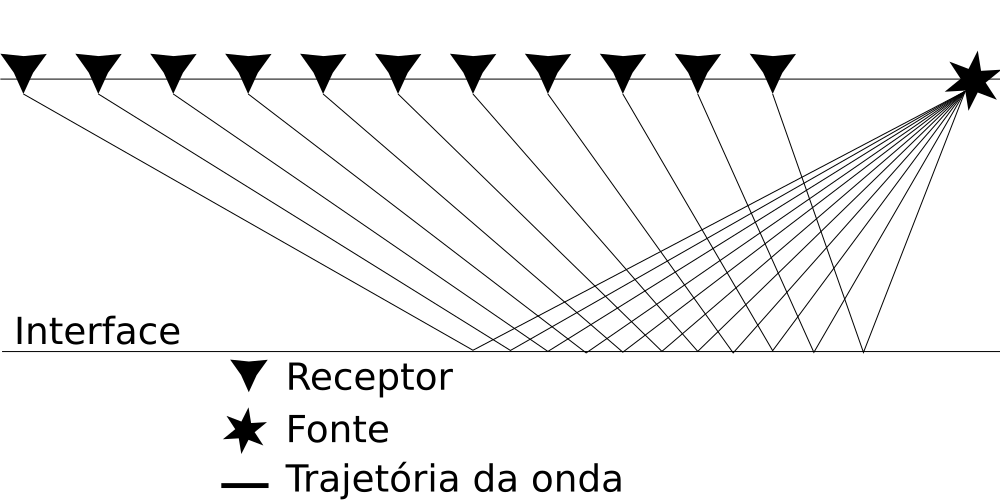
\includegraphics[scale=0.4]{../imagens/shot.png}
        \caption{Configuração de fontes e receptores para traços ordenados no domínio do tiro. Comuns em aquisições convencionais usando cabos suspensos na superfície.}
        \label{shotTrace}
    \end{figure}
    
    \begin{figure}[htp!]
        \centering
        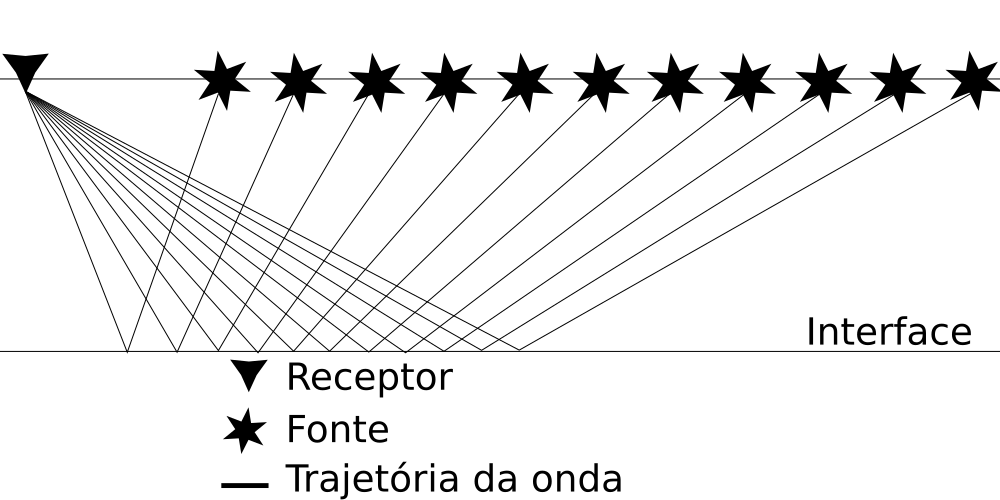
\includegraphics[scale=0.4]{../imagens/recept.png}
        \caption{Configuração de fontes e receptores para traços ordenados no domínio do receptor. Para levantamentos usando técnicas avançadas de coleta de dados, como cabos sensores (OBC) ou receptor único (OBN) no fundo marinho, os traços são organizados no domínio do receptor comum.}
        \label{receptTrace}
    \end{figure}

    \begin{figure}[htp!]
        \centering
        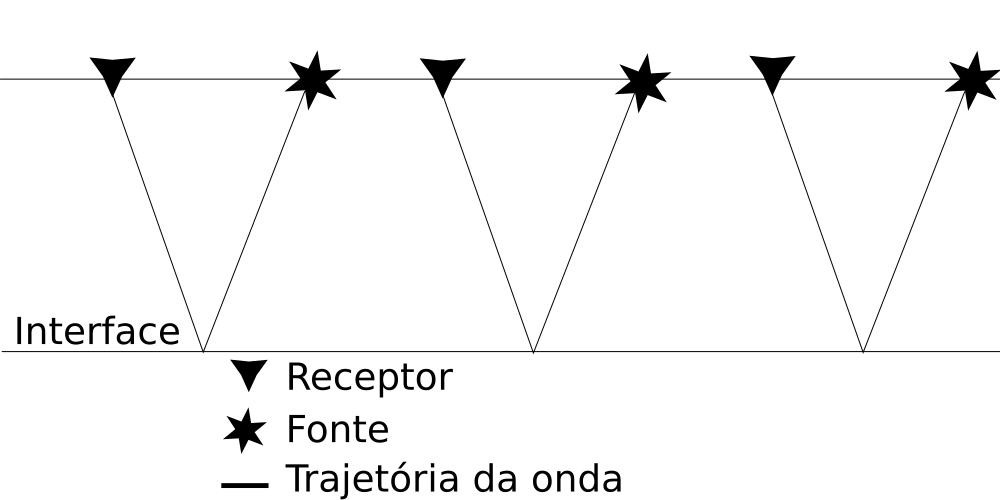
\includegraphics[scale=0.4]{../imagens/offset.png}
        \caption{Configuração de fontes e receptores para traços ordenados no domínio do \textit{offset}. Esse tipo de ordenação é util para observar continuidades laterais nas principais reflexões, para controle de qualidade da aquisição, entre outros.}
        \label{offsetTrace}
    \end{figure}
    
    \begin{figure}[htp!]
        \centering
        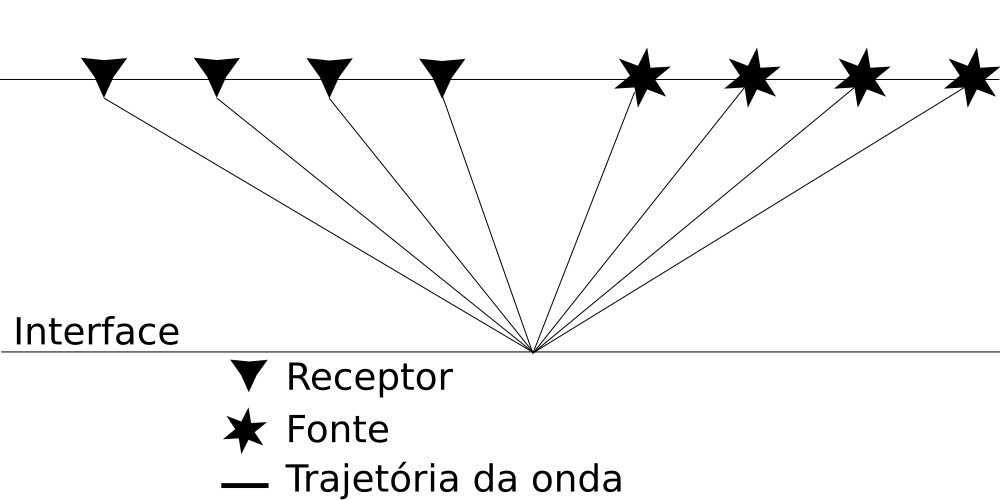
\includegraphics[scale=0.4]{../imagens/cdp.png}
        \caption{Configuração de fontes e receptores para traços ordenados no domínio do ponto médio comum (CMP). Estratégia usada em levantamentos sísmicos convencionais para preparar a etapa de estimativa de velocidades sísmicas.}
        \label{cmpTrace}
    \end{figure}    

	%- Análise de valocidades, velocidade NMO, RMS e INT.
	%- Empilhamento do dado.
    \newpage
    \subsection*{Análise de velocidades e empilhamento}
    
    As curvas formadas em dados sísmicos ordenados no domínio do ponto médio comum tem dimensões de tempo duplo e afastamento fonte-receptor. A figura \ref{cmpGather} mostra a configuração típica de uma seção de ponto médio comum ilustrando quatro refletores com suas hipérboles de reflexão. A equação que aproxima as curvas hiperbólicas de um dado sísmico no domínio do ponto médio tem a seguinte forma
%    
    \begin{equation}
        T^2(x) = T_0^2 + \dfrac{x^2}{V_{NMO}}
        \label{velan}
    \end{equation}
%    
    \noindent onde $T(x)$ representam os tempos pertencentes à hipérbole, $x$, os afastamentos fonte-receptor, $T_0$, o tempo duplo de menor afastamento e $V_{NMO}$, a velocidade \textit{Normal Move Out} ou sobretempo normal, parâmetro que melhor ajustará a curva hiperbólica. O sobretempo normal é o tempo em que a reflexão demora para atingir os receptores mais distantes em relação ao receptor normal à frente de onda. A velocidade de sobretempo normal pode ser considerada aproximadamente como a velocidade média quadrática, mais conhecida como $V_{RMS}$, quando o meio apresenta camadas plano-paralelas horizontais sem variação lateral de velocidade intervalar em subsuperfície \cite{yilmaz2001seismic}. 

    \begin{figure}[htp!]
        \centering
        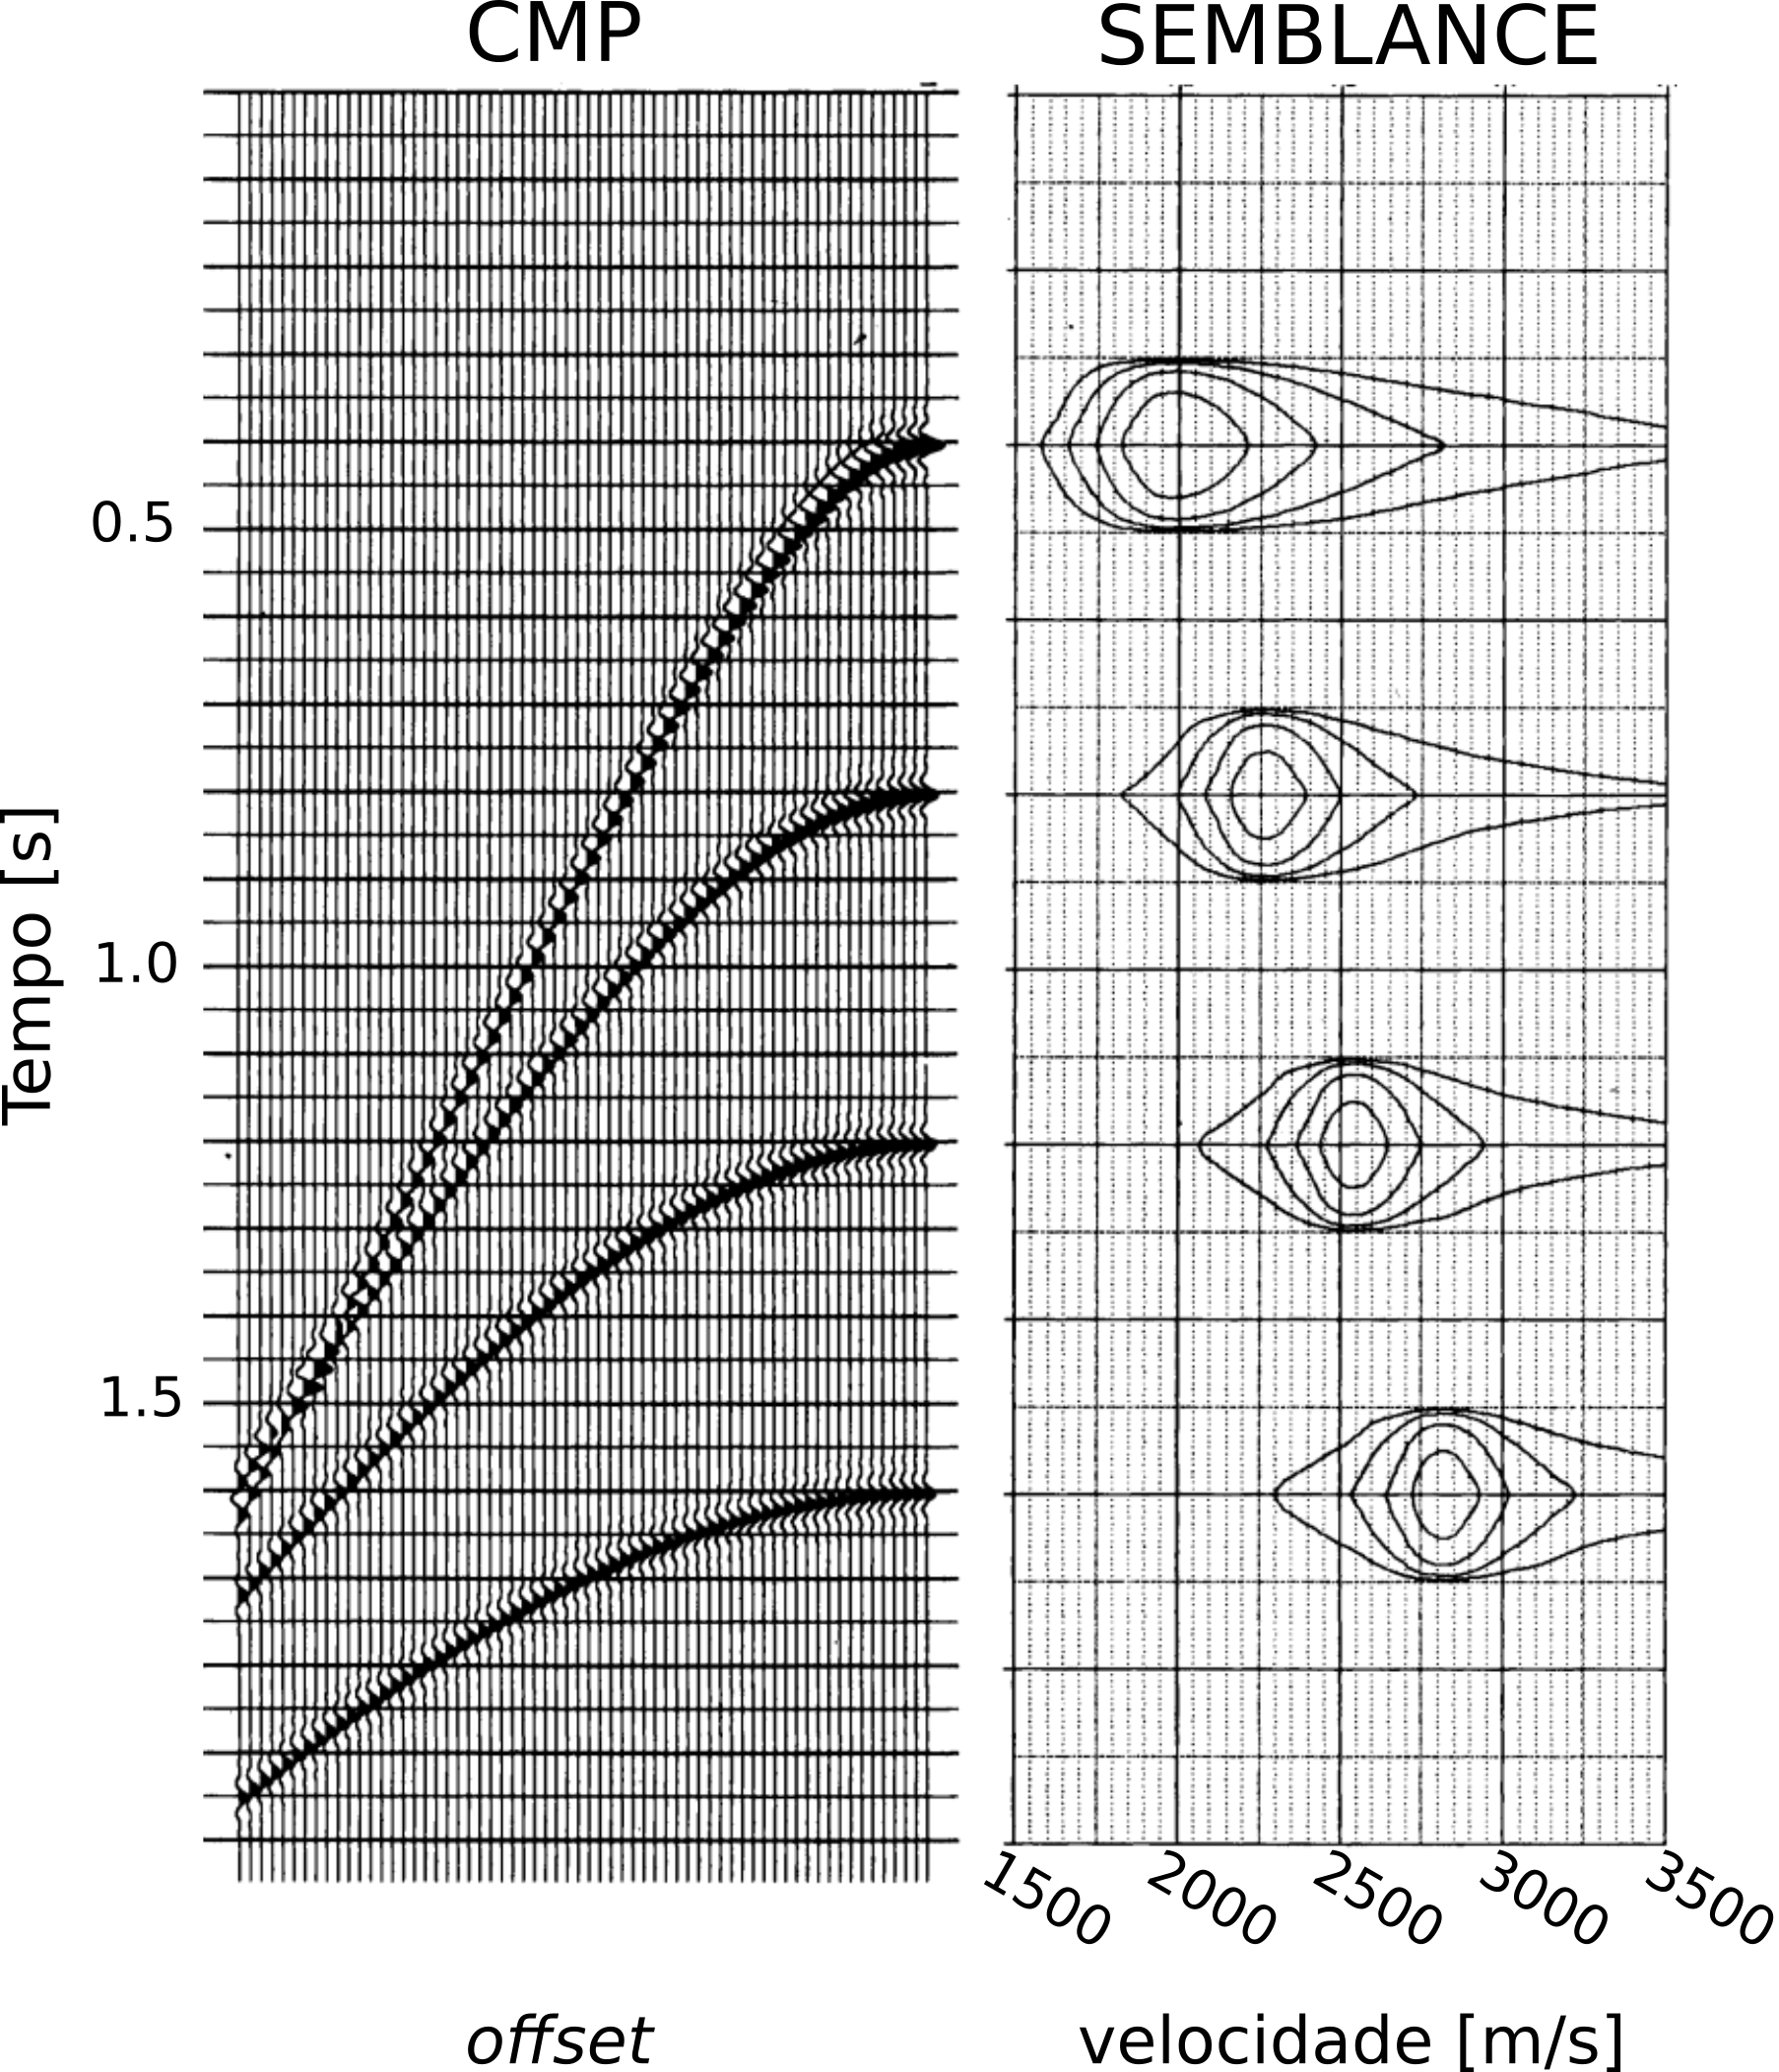
\includegraphics[width=10cm,height=10cm]{../imagens/cmpSemblance.png}
        \caption{CMP é a sigla para \textit{commom mid point} comumente usada para se referenciar às seções de ponto médio comum e o Semblance é a matriz que correlaciona as hipérboles de reflexão do dado CMP com as velocidades NMO. Para cada tempo presente na seção de ponto médio é calculada a correlação de diversas velocidades \textit{Normal Move Out} que melhor ajustam as reflexões do dado CMP (adaptado de \citeonline{yilmaz2001seismic}).}
        \label{cmpGather}
    \end{figure}
    
    A análise de velocidades tem o objetivo de identificar as velocidades que ajustam as hipérboles presentes em um sismograma no domínio do ponto médio comum. O processo se baseia em aplicar a correção do sobretempo normal para uma janela de velocidades médias quadráticas e assim correlacionar as velocidades com os tempos presentes na seção de ponto médio comum. A correlação origina uma matriz chamada \textit{semblance}, onde para cada tempo existe uma janela de velocidade correspondente contendo um certo valor, variando de zero a um. A matriz \textit{semblance} mostra o grau de correlação que a velocidade em questão pode ajustar ou horizontalizar a curva hiperbólica para um certo tempo do sismograma de ponto médio comum.
    
    Usando a premissa da análise de velocidades e horizontalizando as curvas hiperbólicas, parte-se para o próximo passo, validar parcialmente as velocidades estimadas. Tal processo é chamado de empilhamento (figura \ref{empilhamento}), que consiste em mapear todos os pontos médios que contemplam a aquisição e usando as seções de pontos médios com o sobretempo normal corrigidos, soma-se toda a energia dos traços pertencentes àquela seção. O empilhamento de traços transforma uma seção de ponto médio comum em um único traço contendo a energia acumulada das reflexões. Portanto, a horizontalização dos eventos é de suma importância para o processo de empilhamento e consequentemente, a estimativa de velocidade deve ser o mais precisa possível.
    
    \begin{figure}[htp!]
    	\centering
    	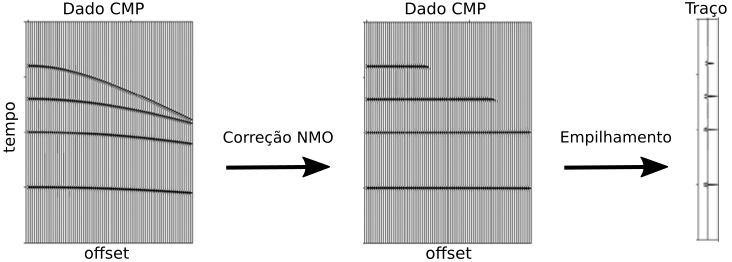
\includegraphics[width=15cm,height=6.5cm]{../imagens/empilhamento.png}
    	\caption{Empilhamento de dados sísmicos para um CMP. A correção NMO horizontaliza os eventos, uma função que silencia os traços de \textit{offsets} longos é criada para corrigir o efeito do \textit{stretching} (causado pela correção NMO) e assim os traços são somados dando origem a um único traço pelo processo de empilhamento (adaptado de \citeonline{yilmaz2001seismic}).}
    	\label{empilhamento}
    \end{figure}
    
    A velocidade intervalar é a grandeza presente no meio de propagação da onda. O objetivo da estimativa de velocidade seria obter a velocidade intervalar, pois com o processo de análise de velocidades se obtém aproximadamente a média quadrática das velocidades do meio (velocidade RMS) exigindo-se uma conversão. Existem atualmente alguns outros métodos mais robustos para a obtenção das velocidades como a tomografia sísmica \cite{bishop1985tomographic} e a inversão completa do campo de onda \cite{tarantola1984inversion}, porém esses métodos, além de mais complexos, necessitam de um campo de velocidades inicial. A análise de velocidades, citada neste trabalho, foi o método utilizado para a obtenção do campo de velocidades, pois a região em questão se mostra parcialmente concordante com as premissas do método. As equações de conversão das velocidades citadas anteriormente são formuladas da seguinte maneira \cite{dix1955seismic,yilmaz2001seismic}
    
    \begin{equation}
        \begin{cases}
            \bigskip V_{INT}[i] =  \sqrt{\left(\dfrac{V_{RMS}^2[i] t[i] - V_{RMS}^2[i-1] t[i-1]}{t[i] - t[i-1]}\right)}  \\
            V_{NMO}[i] \approx V_{RMS}[i] = \sqrt{\left(\dfrac{\displaystyle\sum V_{INT}^2[i]t[i]}{\displaystyle\sum t[i]}\right)},
        \end{cases}
        \label{dix}
    \end{equation}

    \noindent onde para o cálculo da velocidade intervalar $V_{INT}$, se usa a velocidade média quadrática $V_{RMS}$ ao quadrado até a camada $i$ e o tempo duplo total $t$ até a camada $i$. Para o cálculo da velocidade média quadrática $V_{RMS}$, se usa o somatório da velocidade intervalar $V_{INT}$ ao quadrado até a camada $i$ e o tempo intervalar $t$ pertencente à camada $i$.
    
\section{Modelagem sísmica para meios elásticos isotrópicos}

	Representar a propagação de uma onda no espaço requer certas simplificações, pois o meio real é extremamente complexo. Uma simplificação para propagação de ondas em sólidos seria o caso elástico isotrópico, onde a vibração das partículas não afeta a quantidade de energia da onda e, por ser isotrópico, a onda se propaga igualmente para todas as direções \cite{aki2002quantitative}. Para entender como o meio se comporta a partir de uma passagem de energia, os conceitos de tensão e deformação são essenciais, pois as equações governantes são geradas através dessas grandezas.   

	Cada componente em um sistema de movimento experimenta alguma forma de carga devido a forças aplicadas em certa direção. A tensão é definida pela razão da força aplicada por unidade de área. Dependendo da direção de aplicação, pode ser classificada por tensão de tração, que tende a esticar ou alongar o material, tensão compressiva, que tende a comprimir ou encurtar o material, e tensão cisalhante, que tende a deformar o material \cite{achenbach1973applied,pujol2003elastic}. A figura \ref{stress} mostra o diagrama das possíveis forças de tensão $\sigma$ atuando num cubo infinitesimal \cite{sanchez2019propagation} e a figura \ref{strain}, exemplifica um tipo de deformação que o material pode sofrer na presença de tensões cisalhantes \cite{sperling2005introduction}. Então, definindo matematicamente a deformação $\varepsilon$, como sendo a derivada do deslocamento de partícula $\vec{u} = (u_x,u_y,u_z)$ em relação a uma direção do espaço cartesiano $(x,y,z)$, tem-se as deformações normais no formato 
	
	\begin{equation}
	 	\varepsilon_{xx} = \dfrac{\partial u_x}{\partial x}; \,\,\,\,\, 
		\varepsilon_{yy} = \dfrac{\partial u_y}{\partial z}; \,\,\,\,\, 
		\varepsilon_{zz} = \dfrac{\partial u_z}{\partial z}, 
	\end{equation}
	
	\noindent e as deformações cisalhantes
	
	\begin{equation}
	 	\varepsilon_{zx} = \varepsilon_{xz} =  \dfrac{1}{2}\left(\dfrac{\partial u_z}{\partial x} + \dfrac{\partial u_x}{\partial z}\right); 
	\end{equation}
	
	\begin{equation}
		\varepsilon_{yx} = \varepsilon_{xy} =  \dfrac{1}{2}\left(\dfrac{\partial u_y}{\partial x} + \dfrac{\partial u_x}{\partial y}\right); 
	\end{equation}
	
	\begin{equation}
		\varepsilon_{zy} = \varepsilon_{yz} =  \dfrac{1}{2}\left(\dfrac{\partial u_z}{\partial y} + \dfrac{\partial u_y}{\partial z}\right). 
	\end{equation}

	As relações entre tensão e deformação são primordiais para a simplificação de propagação de ondas em meios elásticos, pois o meio é completamente elástico no domínio da elasticidade linear \cite{achenbach1973applied,pujol2003elastic,di2010modelagem}, onde a lei de Hooke é aplicável (figura \ref{stressStrain}). 

    \begin{figure}[htp!]
		\centering
		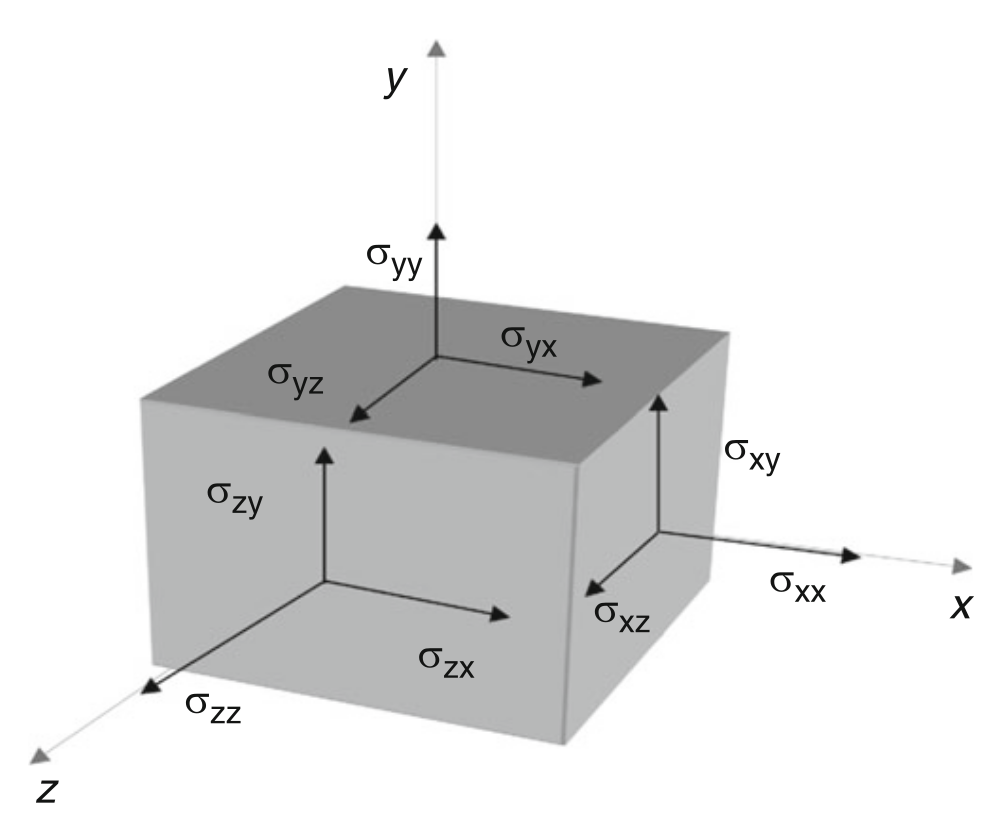
\includegraphics[width=9.5cm,height=8cm]{../imagens/stress.png}
		\caption{Diagrama de todas as tensões, tanto normais $(\sigma_{xx},\,\sigma_{yy},\,\sigma_{zz})$ quanto cisalhantes $(\sigma_{xy},\,\sigma_{xz},\,\sigma_{yx},\,\sigma_{yz},\,\sigma_{zy},\,\sigma_{zx})$, aplicadas num cubo em relação ao espaço cartesiano (adaptado de \citeonline{sanchez2019propagation}).}
		\label{stress}
	\end{figure}

    \begin{figure}[htp!]
		\centering
		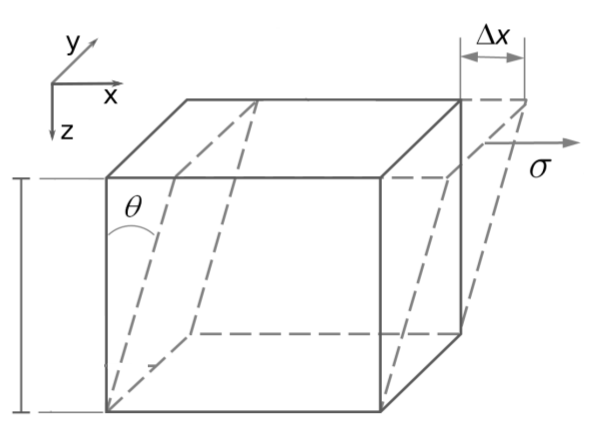
\includegraphics[width=10cm,height=7cm]{../imagens/shear.png}
		\caption{Exemplo de uma tensão cisalhante arbitrária aplicada num cubo, causando deformação e gerando um deslocamento $\Delta x$ do seu estado inicial (adaptado de \citeonline{sperling2005introduction}).}
		\label{strain}
	\end{figure}

	A teoria sobre mecânica dos materiais tem suas particularidades e está amplamente descrita em livros e teses como nos trabalhos de \citeonline{achenbach1973applied}, \citeonline{pujol2003elastic}, \citeonline{aki2002quantitative}, \citeonline{alsadi2017seismic}, nos apêndices do \citeonline{yilmaz2001seismic} e, uma referência brasileira, o trabalho de \citeonline{di2010modelagem}.
	
	 Estes autores abordam toda a teoria tensorial e conservação da quantidade de movimento para deduzir a equação geral linearizada para a propagação da onda em meios elásticos pela lei de Hooke e segunda lei de Newton generalizadas. 

    \begin{figure}[htp!]
		\centering
		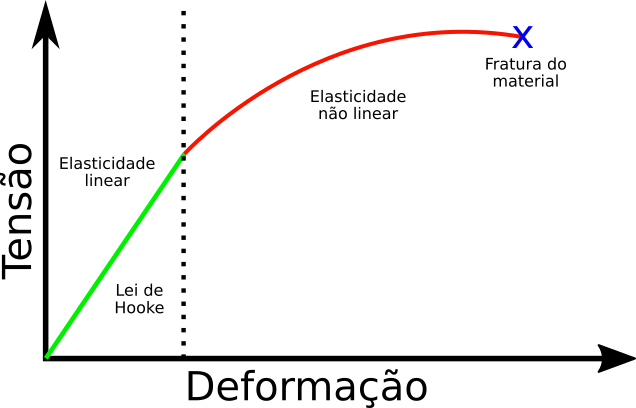
\includegraphics[width=10cm,height=6cm]{../imagens/stressStrain.png}
		\caption{Relação entre tensão e deformação. Lei de Hooke válida somente até o limite da elasticidade linear (adaptado de \citeonline{kearey}).}
		\label{stressStrain}
	\end{figure}

	As equações da onda podem ser representadas por campo único, onde se considera os deslocamentos de partícula como campo de onda ou por campo duplo, considerado a velocidade ou deslocamentos de partícula e as tensões como campos de onda. Na prática, as equações de campo duplo são mais utilizadas para modelar o fenômeno de propagação de ondas em meio elástico, que serão apresentadas a seguir.
		
\subsection*{Equação governante}

	Neste trabalho, será utilizado o sistema de equações de primeira ordem relacionando velocidades de partícula e tensões para simular a propagação da onda em meio elástico isotrópico em duas dimensões. O trabalho de \citeonline{virieux1986p}, mostra a equação, a solução numérica pelo método das diferenças finitas e aborda detalhadamente as condições de estabilidade e não dispersão numéricas. Já em \citeonline{levander1988fourth}, é relacionada a posição de cada componente do campo de ondas na malha intercalada numérica, diferenciando dois tipos de configuração e apresentando operadores de derivadas numéricas em quarta ordem no espaço e segunda ordem no tempo. 
	
	Seja $\vec{v}(x,z) = (v_x,v_z)$ as velocidades de partícula, $\vec{\sigma}(x,z) = (\sigma_{xx},\sigma_{zz},\sigma_{xz})$, as tensões presentes no caso 2D, $\lambda(x,z) = \lambda$, a constante de compressibilidade, $\mu(x,z) = \mu$, o parâmetro de cisalhamento e $\rho(x,z) = \rho$, a densidade do meio, a equação governante do problema segue o formato 
%
	\begin{equation}
		\begin{cases}
			\rho\partial_t v_x = \partial_x \sigma_{xx} + \partial_z \sigma_{xz} \\
			\rho\partial_t v_z = \partial_x \sigma_{xz} + \partial_z \sigma_{zz} \\
			\partial_t \sigma_{xx} = (\lambda + 2\mu) \partial_x v_x + \mu\partial_zv_z, \\
			\partial_t \sigma_{zz} = (\lambda + 2\mu) \partial_z v_z + \mu\partial_xv_x \\
			\partial_t \sigma_{xz} = \mu(\partial_xv_z + \partial_zv_x)
		\end{cases}
		\label{elasticWave}
	\end{equation}
%
	\noindent sendo $\partial_t$ a derivada parcial em relação ao tempo e $(\partial_x,\partial_z)$ derivadas em relação ao espaço. As constantes de Lamé são calculadas através das relações
%
	\begin{equation}
		\begin{cases}
			\mu = \rho v_s^2 \\
			\lambda = \rho v_p^2 - 2\mu.
		\end{cases}
	\end{equation}
%
	A velocidade da onda compressional $v_p$ será estimada a partir do dado sísmico e a velocidade da onda cisalhante $v_s$ será aproximada a partir da relação mostrada em \citeonline{kearey}, onde para rochas bem consolidadas com razão de Poisson em torno de $\nu = 0.25$, $v_p$ se relaciona com $v_s$ da seguinte maneira
%
	\begin{equation}
		v_p = \left[\dfrac{2(1-\nu)}{1 - 2\nu}\right]^{\frac{1}{2}}v_s \,\,\,\,\rightarrow\,\,\,\, v_p \approx 1,7 v_s. 
	\end{equation}  
%
	A densidade também será estimada através da velocidade $v_p$, utilizando a relação de \citeonline{gardner1974formation} para rochas em meio poroso. Então para uma velocidade medida em $m/s$, a densidade em $kg/m^3$ é dada pela equação
%
	\begin{equation}
		\rho = 310 \,v_p^{0,25}.	
	\end{equation}
%
	Sabendo a equação no caso contínuo, basta identificar algum método numérico para solucionar o problema computacionalmente e o procedimento utilizado neste trabalho será o método das diferenças finitas.

\subsection*{Método das diferenças finitas}

	Existe um vasto conhecimento sobre a simplificação de funções contínuas para o domínio computacional discreto \cite{oppenheim1999discrete,hayes1999schaum}, onde um meio que continha infinitos pontos passa a ter somente alguns pontos espaçados regularmente por um parâmetro de discretização $h$ (Figura \ref{mdf1d}). Em equações diferenciais as variáveis são funções. Então, o objetivo a ser alcançado ao resolver uma equação diferencial numericamente é encontrar uma aproximação discreta que satisfaça a relação entre as derivadas em
	alguma determinada região do espaço e/ou tempo, juntamente com algumas condições de contorno ao longo das bordas deste domínio \cite{leveque1998finite}.
%
    \begin{figure}[htp!]
		\centering
		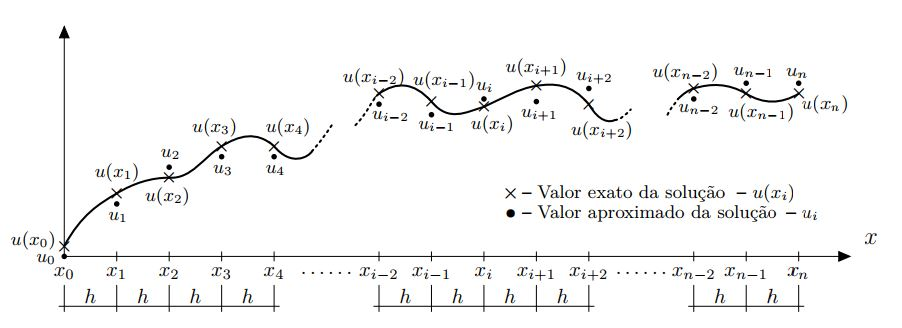
\includegraphics[width=16cm,height=6cm]{../imagens/1.jpg}
		\caption{Ilustração da discretização de uma função solução unidimensional $u(x)$. A linha sólida é a representação da função no caso contínuo, as marcações em $\times$ representam valores analíticos da função solução nos pontos discretizados e as marcações em $\bullet$ representam da solução numérica, uma aproximação de $u(x)$ discreta (adaptado de \citeonline{ruas2016numerical}).}
		\label{mdf1d}
	\end{figure}
%

	O método das diferenças finitas se baseia na série de Taylor, onde sabendo-se as derivadas da função no ponto $x_0$ consegue-se estimar o valor de $f(x)$ no ponto $x_0$. Sendo  $f^{(n)}(x_0)$ as derivadas de $f(x)$ em relação a $x_0$ de ordem $n$, o cálculo de $f(x)$ é dado no formato   
%
	\begin{equation}
		f(x) = \displaystyle\sum_{n=0}^{\infty} \dfrac{f^{(n)} (x_0)}{n!}(x - x_0)^n.
	\end{equation}
%
	\noindent Contudo, a utilização no método das diferenças finitas se resume na estimativa de pontos na redondeza de $x_0$ conhecendo o valor da função e suas derivadas no ponto $x_0$. 
	
	Esse resultado é alcançado realizando a substituição de $x = x_0+h$ no argumento da série, a transformando em
%
	\begin{equation}
		f(x_0 + h) = \displaystyle\sum_{n=0}^{\infty} \dfrac{f^{(n)} (x_0)}{n!}(x_0 + h - x_0)^n = \displaystyle\sum_{n=0}^{\infty} \dfrac{f^{(n)} (x_0)}{n!}(h)^n.
	\end{equation}
%
	\noindent Expandindo a série até a derivada de primeira ordem, tem-se	
%
	\begin{equation}
		f(x_0 + h) = f(x_0) + f'(x_0)h + \mathcal{O}(h^2).
		\label{finDiff}
	\end{equation}
%	
	O erro de truncamento $\mathcal{O}(h^2)$ significa que a aproximação do valor da função em $x_0+h$ terá um erro de $\pm h^2$. Então, para ser mais preciso na estimativa das derivadas, o parâmetro de discretização $h$ deve ser pequeno \cite{leveque1998finite}. Ao ignorar o erro de truncamento, rearranjando a equação \ref{finDiff}, sabendo que a aproximação em diferenças finitas pode ser progressiva $(D^+)$, regressiva $(D^-)$ e central $(D^o)$, dependendo dos pontos de referência em relação à $x_0$ e $h$ (Figura \ref{derivadas}), tem-se as equações abaixo 
%
	\begin{equation}
		\begin{cases}
			D^+\{f(x_0)\} \approx \left[f(x_0 + h) - f(x_0)\right] / h \\
			D^-\{f(x_0)\} \approx \left[f(x_0) - f(x_0 - h)\right] / h \\
			D^o\{f(x_0)\} \approx \left[f(x_0 + h) - f(x_0 - h)\right] / 2h. 
		\end{cases}
		\label{difMDF}
	\end{equation}
%
 	As derivadas de diferentes ordens podem ser aproximadas por diferenças finitas, porém o problema a ser resolvido neste trabalho necessita somente das derivadas de primeira ordem, já que o sistema de equações \ref{elasticWave} possui derivadas de primeira ordem. 
%
    \begin{figure}[htp!]
		\centering
		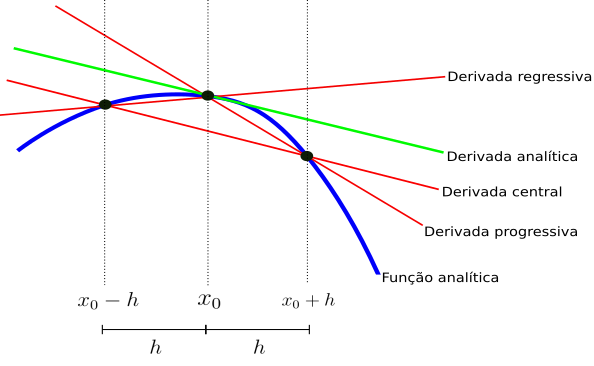
\includegraphics[width=13cm,height=8.5cm]{../imagens/derivadas.png}
		\caption{Configuração das retas tangentes considerando os diferentes tipos de derivada numérica comparados à derivada analítica (adaptado de \citeonline{leveque1998finite}).}
		\label{derivadas}
	\end{figure}
%	
 	As diferenças finitas também se aplicam em derivadas parciais seguindo o mesmo raciocínio, porém ao aplicar a derivada em uma direção, as outras ficam livres. Seja $u(x,t)$ uma função dependente do espaço unidimensional $x$ e do tempo $t$, a derivada em relação ao tempo $t$ no instante $t = t_0$ pode ser aproximada da seguinte maneira    
%
 	\begin{equation}
 		\partial_t u(x,t_0)	\approx \left[u(x,t_0+h) - u(x,t_0)\right] / \Delta t
 	\end{equation}  
%	
	\noindent onde $\Delta t$ é o parâmetro de discretização referente à variável $t$ e a parte espacial, dependente de x, permaneceu livre.

	Para se obter operadores de diferenças finitas em ordens superiores, necessita-se que tenha mais pontos para realizar a aproximação da derivada. \citeonline{FDCC}, mostra uma solução interessante para se calcular pragmaticamente os parâmetros de qualquer tipo de diferença finita independente da ordem da derivada ou do operador de diferenças. Basicamente, foi usada a expansão em série de Taylor onde se organiza os coeficientes a partir da configuração de uma matriz e, assim, um sistema linear é resolvido encontrando os coeficientes das diferenças finitas. 
	
\subsection*{Discretização em malha intercalada}
	
	A maneira clássica para obter a resolução do sistema de equações \ref{elasticWave} usando o método das diferenças finitas é por discretização em malha intercalada, abordada no trabalho de \citeonline{levander1988fourth}. O \textit{stencil} de diferenças finitas será centrado nas tensões normais, juntamente com as propriedades elásticas do meio (Figura \ref{staggeredGrid}).
%    
    \begin{figure}[htp!]
		\centering
		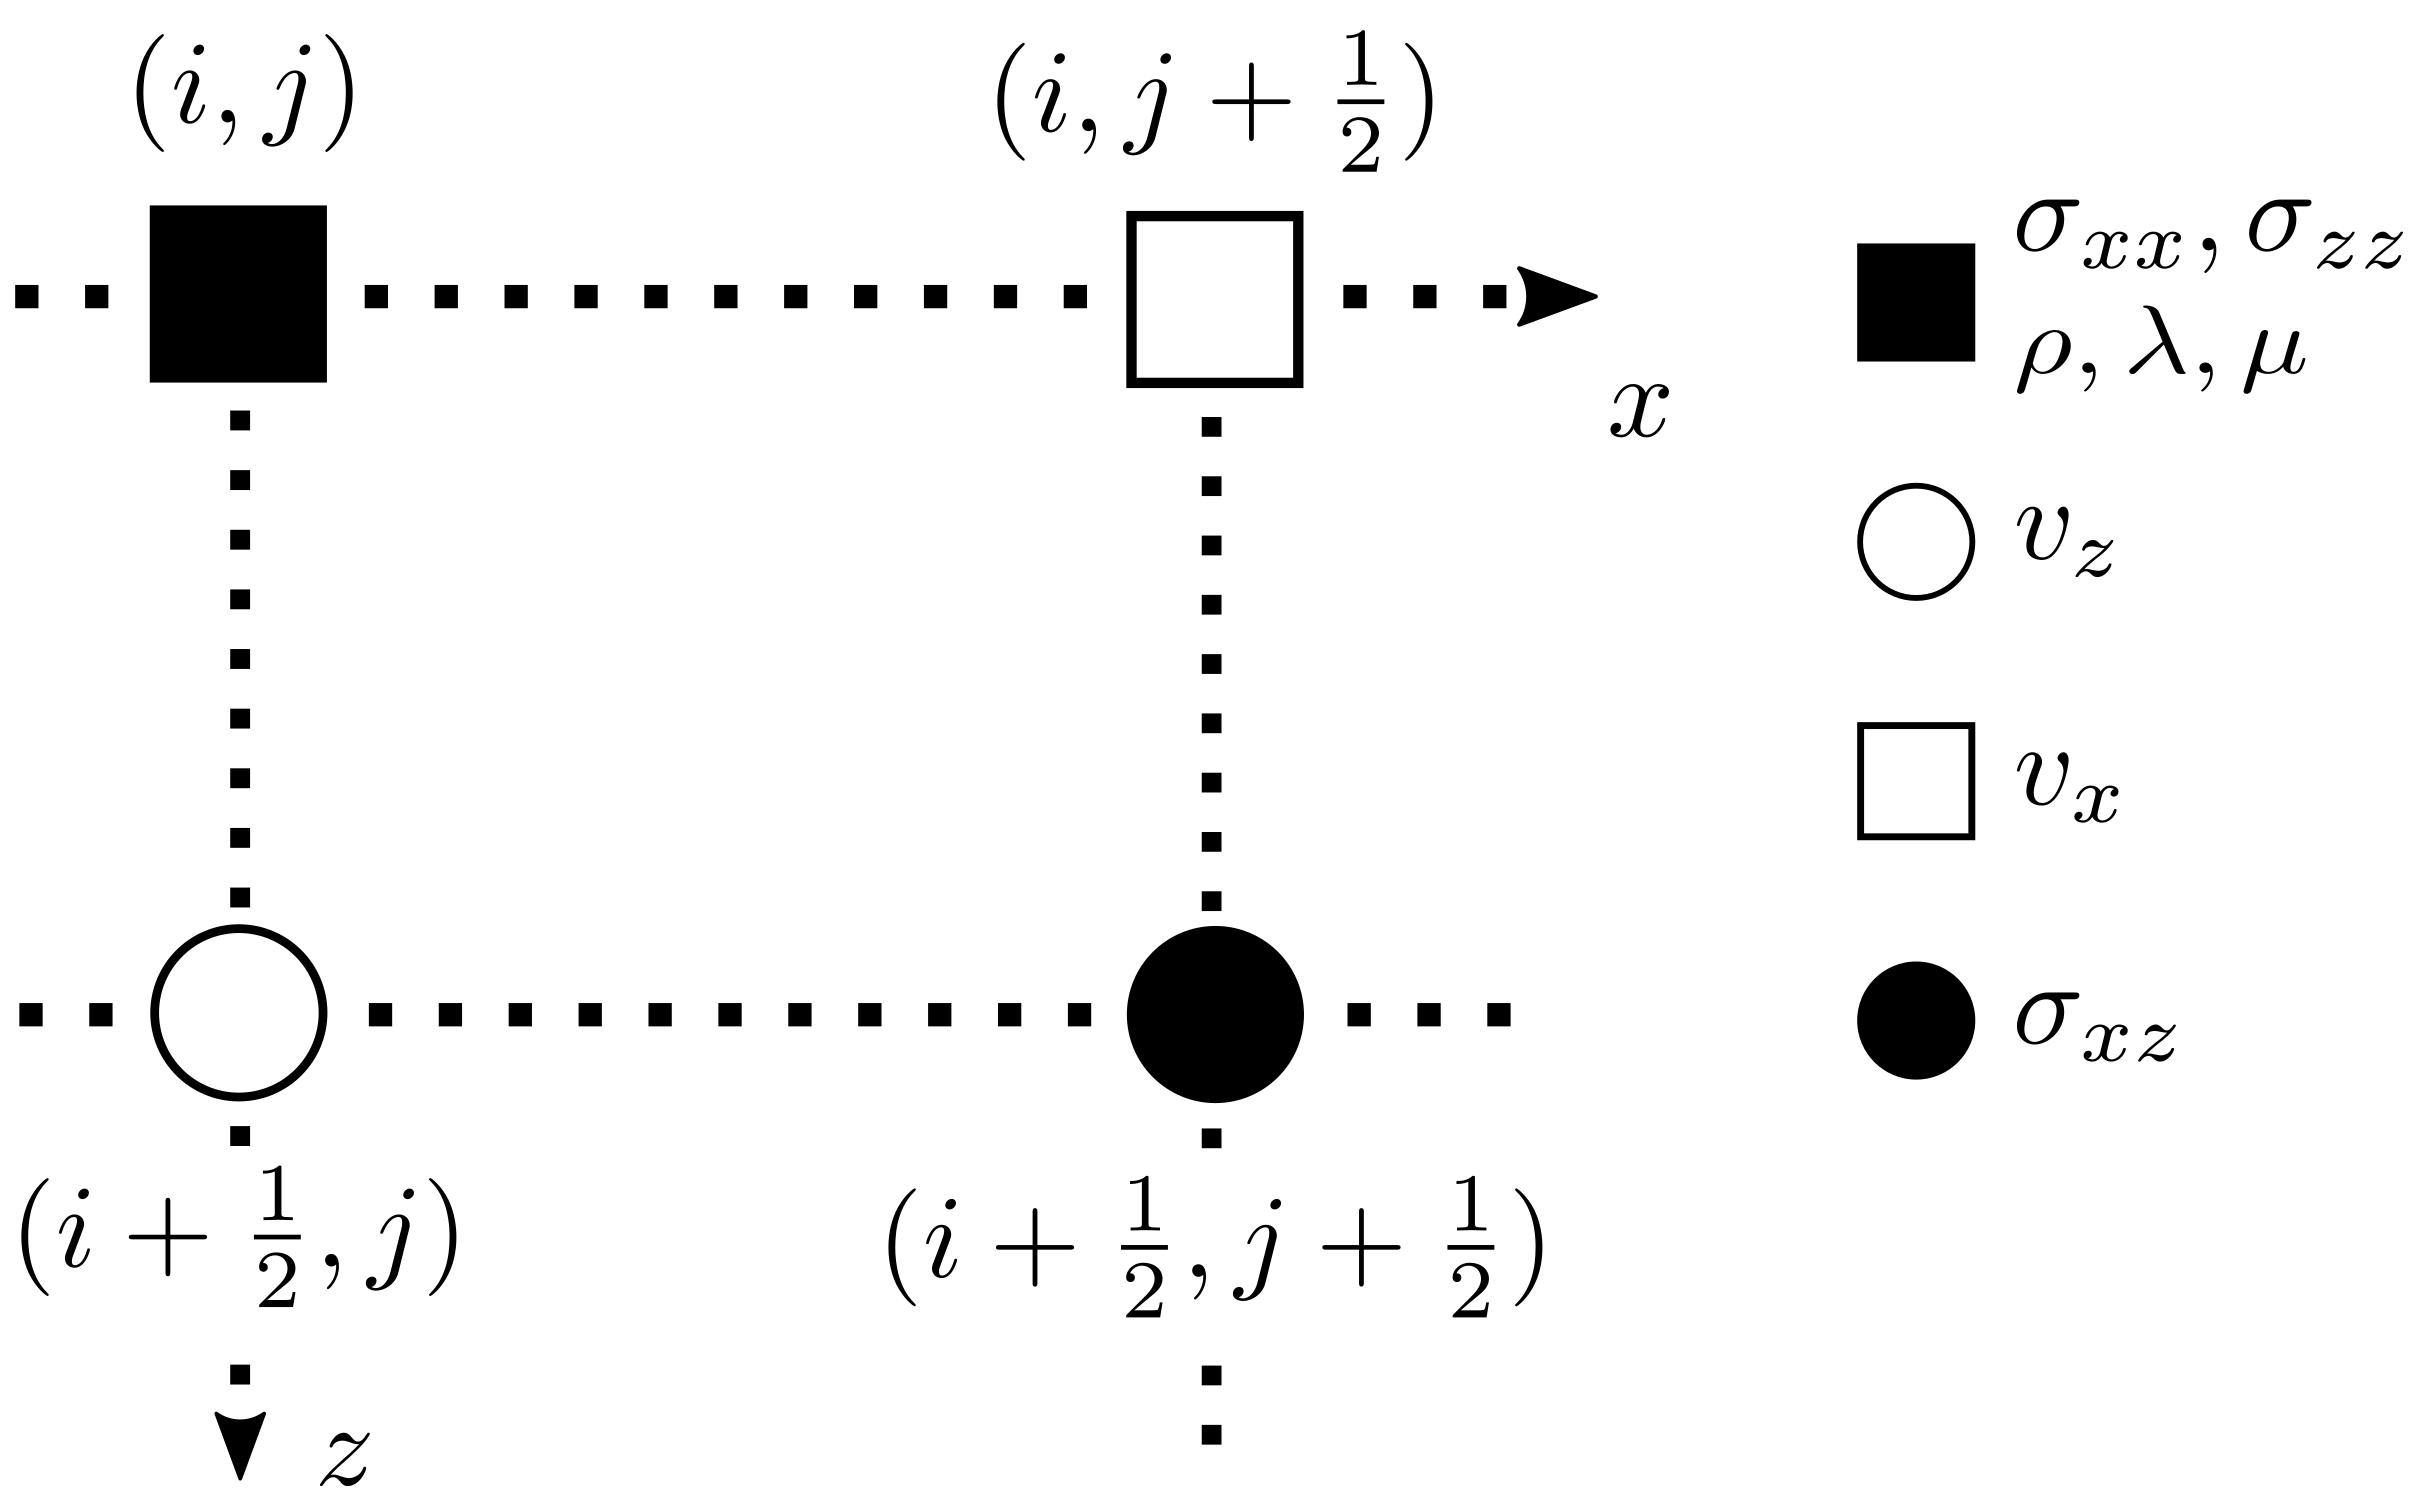
\includegraphics[width=13cm,height=8.5cm]{../imagens/staggeredGrid.png}
		\caption{Esquema de diferenças finitas com \textit{stencil} centrado nas tensões normais. Os parâmetros elásticos do meio $(\rho,\lambda,\mu)$ pertencem apenas ao índice $(i,j)$ (inspirado em \citeonline{levander1988fourth}).}
		\label{staggeredGrid}
	\end{figure}

	Existe uma peculiaridade na aplicação das diferenças finitas utilizando a malha intercalada na resolução do problema da equação \ref{elasticWave}, onde os pontos da malha estão dispostos de $\frac{1}{2}$ em $\frac{1}{2}$ (Figura \ref{staggeredGrid}). Então as diferenças centrais com operadores de segunda ordem seguem o formato
%
	\begin{equation}
		D^o\{f(x_0)\} \approx \left[f(x_0 + 0,5h) - f(x_0 - 0,5h)\right] / h. 
	\end{equation}
%

	\newpage
	Aplicando diferenças finitas centrais em todas as derivadas da equação \ref{elasticWave}, considerando $(v_x, v_z) = (U,V)$ e $(\sigma_{xx},\sigma_{zz},\sigma_{xz}) = (X,Z,T)$, usando $n$ para relacionar o tempo, $i$, a profundidade (direção z), e $j$, a distância (direção x), se obtém
%
	\begin{equation}
		\begin{cases}
			\bigskip	
			U^{n+\frac{1}{2}}_{i,j+\frac{1}{2}} = U^{n-\frac{1}{2}}_{i,j+\frac{1}{2}} + \dfrac{dt}{\rho_x}\left(\dfrac{X^n_{i,j+1} - X^n_{i,j}}{dx} + \dfrac{T^n_{i+\frac{1}{2},j+\frac{1}{2}} - T^n_{i-\frac{1}{2},j+\frac{1}{2}}}{dz}\right);\\	
			\bigskip
			V^{n+\frac{1}{2}}_{i+\frac{1}{2},j} = V^{n-\frac{1}{2}}_{i,j+\frac{1}{2}} + \dfrac{dt}{\rho_z}\left(\dfrac{T^n_{i+\frac{1}{2},j+\frac{1}{2}} - T^n_{i+\frac{1}{2},j-\frac{1}{2}}}{dx} + \dfrac{Z^n_{i+1,j} - T^n_{i,j}}{dz}\right);	\\
			\bigskip
			X^{n}_{i,j} = X^{n-1}_{i,j} + dt\left((\lambda_{i,j} + 2\mu_{i,j})\left( \dfrac{U^n_{i,j+\frac{1}{2}} - U^n_{i,j-\frac{1}{2}}}{dx}\right) + \mu_{i,j}\left(\dfrac{V^n_{i+\frac{1}{2},j} - U^n_{i-\frac{1}{2},j}}{dz}\right)\right);\\		
			\bigskip
			Z^{n}_{i,j} = Z^{n-1}_{i,j} + dt\left((\lambda_{i,j} + 2\mu_{i,j})\left( \dfrac{V^n_{i+\frac{1}{2},j} - V^n_{i-\frac{1}{2},j}}{dz}\right) + \mu_{i,j}\left(\dfrac{U^n_{i,j+\frac{1}{2}} - U^n_{i,j-\frac{1}{2}}}{dx}\right)\right);	\\	
			\bigskip			
			T^{n}_{i+\frac{1}{2},j+\frac{1}{2}} = T^{n-1}_{i+\frac{1}{2},j+\frac{1}{2}} + dt\,\mu_{xz}\left(\dfrac{V^n_{i+\frac{1}{2},j+1} - V^n_{i+\frac{1}{2},j}}{dx} +  \dfrac{U^n_{i+1,j+\frac{1}{2}} - U^n_{i,j+\frac{1}{2}}}{dz}\right),		\\
		\end{cases}
	\end{equation} 
%
	\noindent sendo que $\rho_x, \rho_z, \mu_{xz}$ são médias de pontos vizinhos (Figura \ref{staggeredGridElements}), calculadas a partir das relações:
%
	\begin{equation}
		\begin{cases}
			\rho_x = 0.5(\rho_{i,j} + \rho_{i,j+1}) \\
			\rho_z = 0.5(\rho_{i,j} + \rho_{i+1,j}) \\	
			\mu_{xz} = 0.25(1/\mu_{i,j} + 1/\mu_{i+1,j} + 1/\mu_{i,j+1} + 1/\mu_{i+1,j+1})^{-1}. \\		
		\end{cases}
	\end{equation}

	Foi apresentado o sistema de equações discretizado pelo método das diferenças finitas utilizando operadores de derivada em segunda ordem no tempo e no espaço com seus respectivos parâmetros elásticos ajustados. Na prática, os campos de onda $(v_x,v_x,\sigma_{xx},\sigma_{zz},\sigma_{xz})$ ficam separados, cada campo com suas amostras e a intercalação é feita no laço de repetição espacial das diferenças finitas, que será apresentado em breve.
 	
 	Os operadores usados neste trabalho para a aproximação das derivadas foram de segunda ordem no tempo e oitava ordem no espaço. Usando o programa de \citeonline{FDCC}, foram coletados os coeficientes dos operadores em malha intercalada seguindo a lógica de intercalação mostrada em \citeonline{levander1988fourth}. O operador de oitava ordem tem o seguinte formato
%
 	\begin{equation}
		\begin{split}
			f'(x) \approx \dfrac{1}{107520\,h}[75(f(x-3,5h)-f(x+3,5h)) + 1029(f(x+2,5h)-f(x-2,5h))\,\,+\\
			+\,\,\, 8575(f(x-1,5h)-f(x+1,5h)) + 128625(f(x+0,5h)-f(x-0,5h))].				
		\end{split}	
 	\end{equation}
% 	 
    \begin{figure}[htp!]
		\centering
		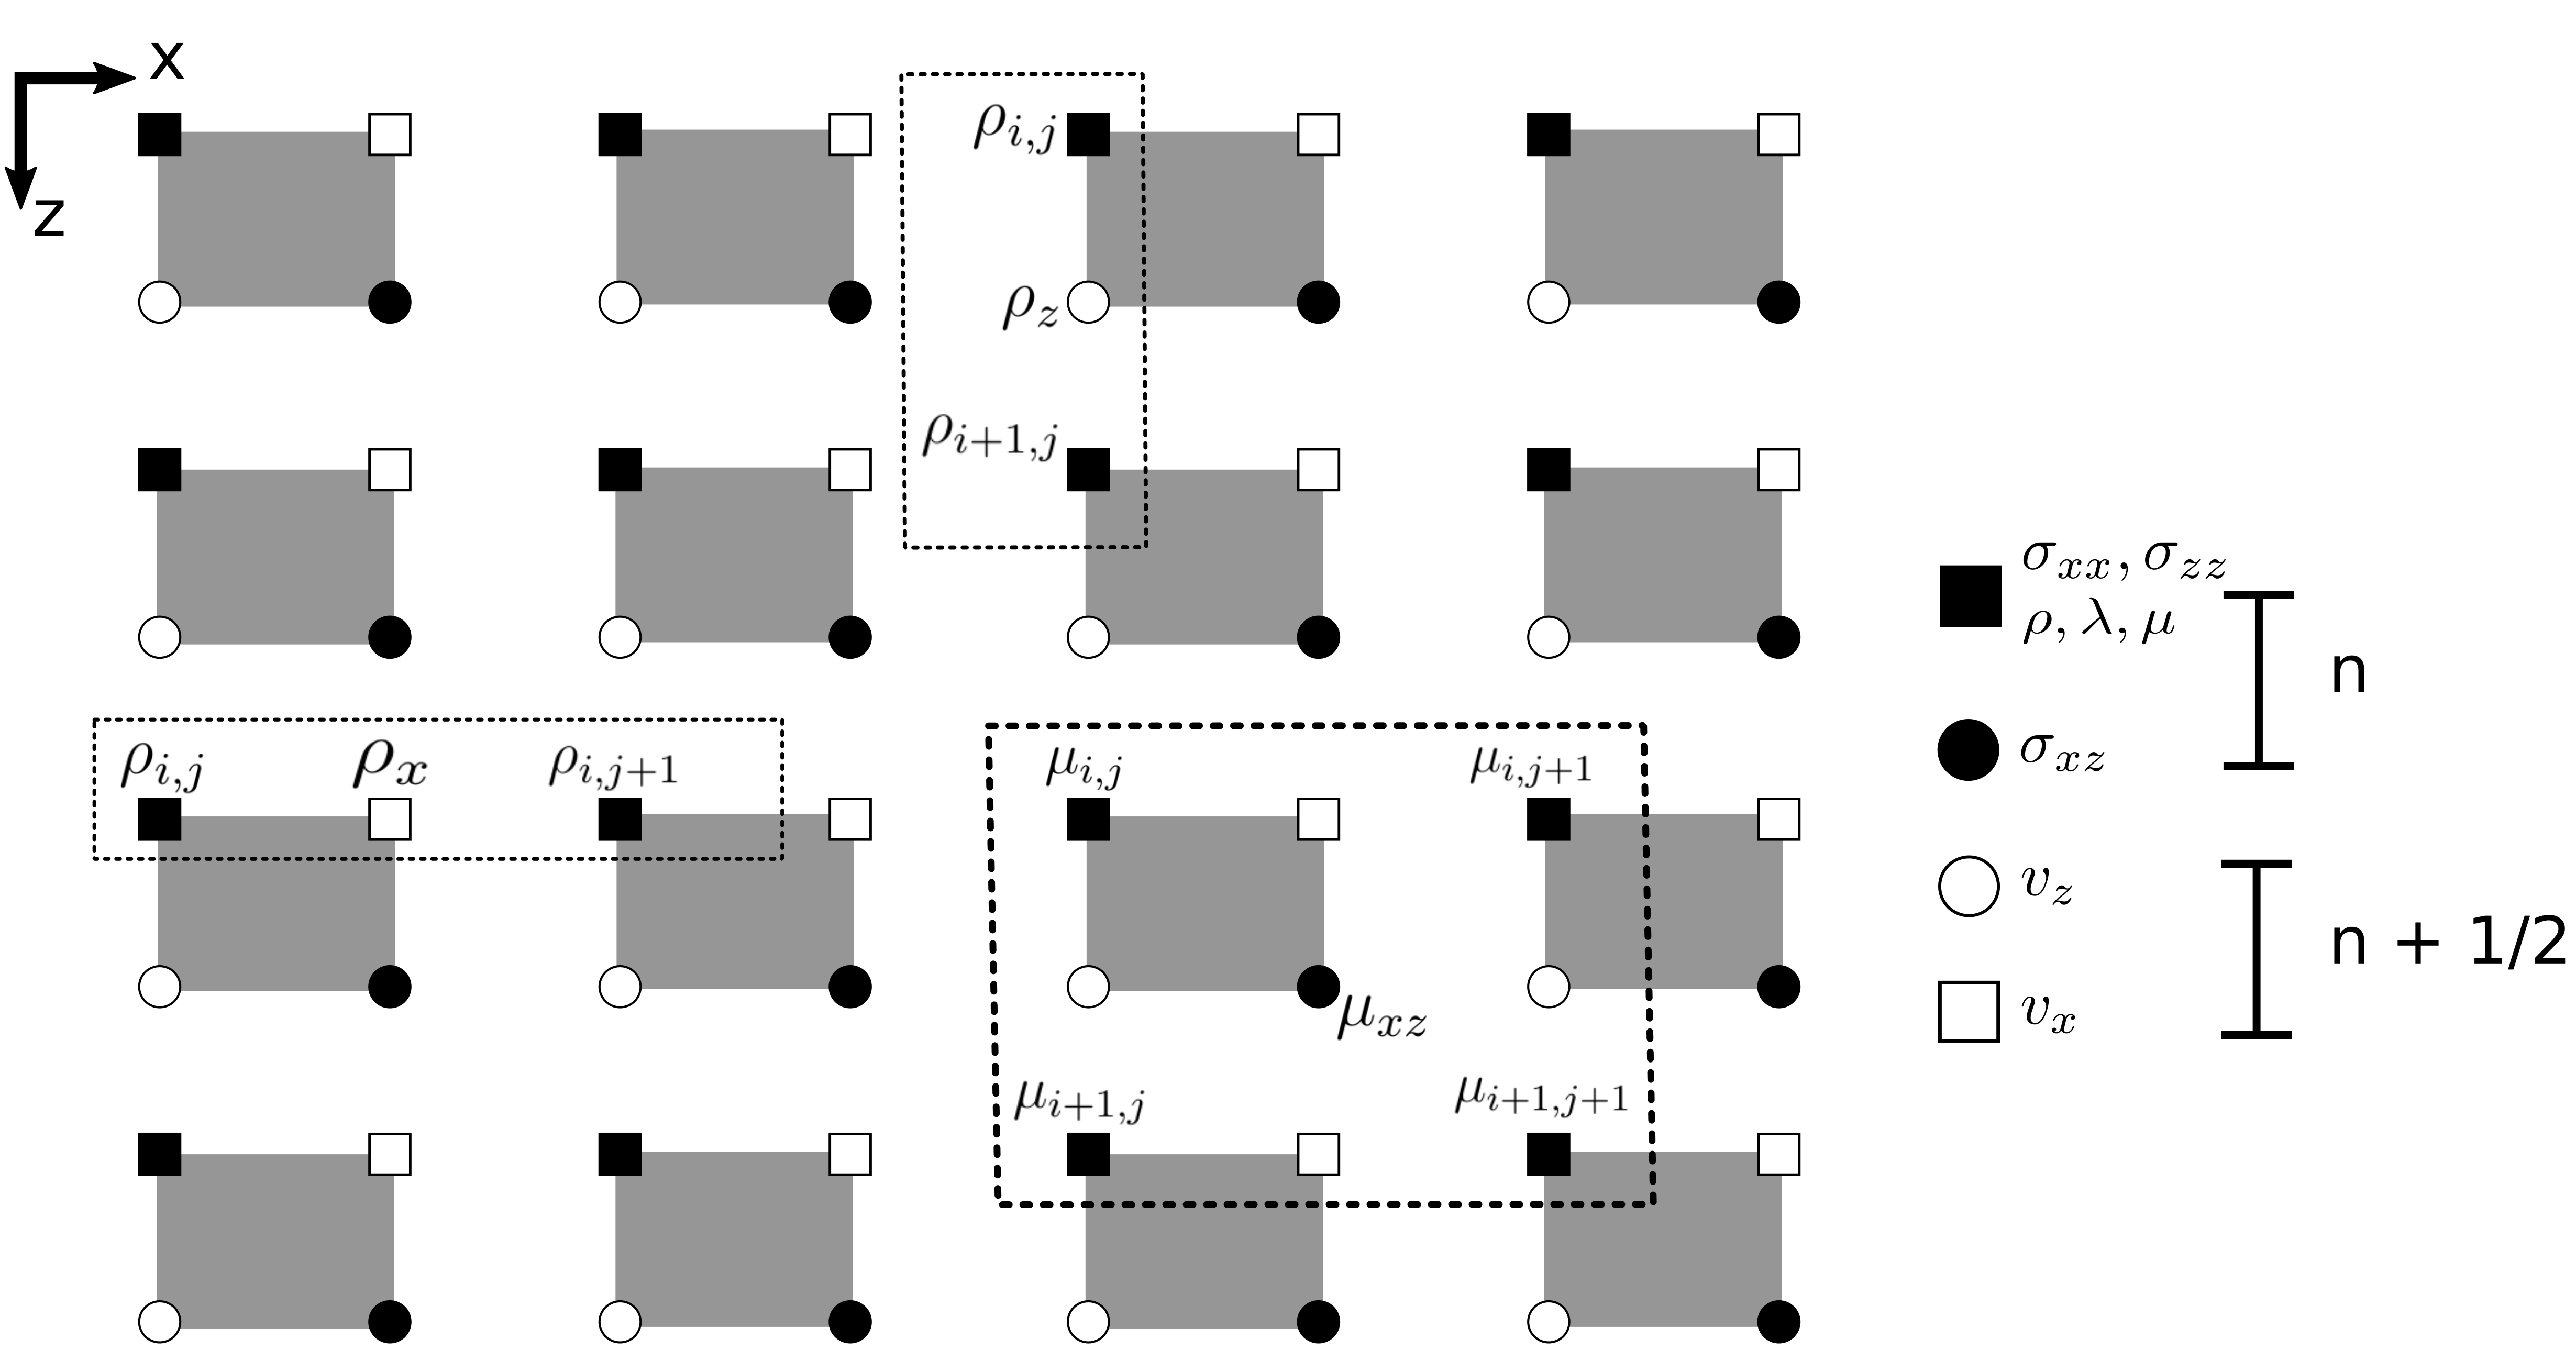
\includegraphics[width=11cm,height=6cm]{../imagens/staggeredGridElements.png}
		\caption{Configuração dos elementos da malha intercalada ilustrando a aproximação dos parâmetros elásticos em pontos da malha onde estes não estão definidos. As tensões são calculadas no instante de tempo $n$ e as velocidades no instante $n+\frac{1}{2}$, ou seja, no mesmo laço de repetição do tempo, as tensões são calculadas primeiro e posteriormente as velocidades.}
		\label{staggeredGridElements}
	\end{figure}

	Sabendo que um \textit{array} 2D pode ser representado por um \textit{array} 1D no formato
%
	\begin{equation}
		\begin{bmatrix}
			a_{0,0} & a_{0,1} & a_{0,2} \\
			a_{1,0} & a_{1,1} & a_{1,2} \\
			a_{2,0} & a_{2,1} & a_{2,2} \\ 
		\end{bmatrix} \to 
		\begin{bmatrix}
			a_{0,0} & a_{0,1} & a_{0,2} &
			a_{1,0} & a_{1,1} & a_{1,2} &
			a_{2,0} & a_{2,1} & a_{2,2}
		\end{bmatrix},
	\end{equation}
%	
	\noindent chamando o número de colunas do \textit{array} 2D de $nc = 3$, as linhas de $i$ e as colunas de $j$, a indexação de acesso no \textit{array} 1D segue na forma
%
	\begin{equation}
		\begin{cases}
			index = i\cdot nc + j \\
			i = index \,\,/ \,\,nc \\
			j = index\,\,\, \% \,\,\,nc,
		\end{cases}
	\end{equation}
%	
	\noindent onde $index$ será a posição do elemento $a_{i,j}$ no \textit{array} 1D. Relacionando o índice $i$ com a divisão de $index$ pelo número de colunas e $j$ pelo resto da divisão de $index$ pelo número de colunas do \textit{array} 2D, tem-se completo a configuração da indexação de matrizes por vetores no domínio computacional. Exemplificando para o elemento $a_{1,2}$ na posição 5, tem-se 
%
	\begin{equation}
		ind[a_{1,2}] = 1\cdot nc + 2 = 1\cdot 3 + 2 = 5.
	\end{equation}	

	As variáveis $nxx$ e $nzz$ como dimensões espaciais do modelo na direção $x$ e $z$ respectivamente, $Vx,Vz,Txx,Tzz,Txz$ como campos de onda, $rho,M,L$ como constantes elásticos, $dx,dz$ como parâmetros de discretização espaciais e $dt$ temporal representam o código base de propagação. Então, o \textit{script} escrito em linguagem C, usando a representação de matrizes por \textit{arrays} 1D, discretizado com operadores de diferenças finitas de segunda ordem no tempo e espaço, e utilizando o \textit{stencil} centralizado nas tensões normais está presente no apêndice A.

\subsection*{Condição numérica de estabilidade e não dispersão}

	A resolução de problemas numéricos são aproximações e estas contém um erro associado. Então, as condições de estabilidade fornecem a informação de consistência da solução e a condição de dispersão numérica mostra a precisão da solução, pois os estes efeitos causam deformações indesejadas na propagação da onda.   

	Segundo \citeonline{virieux1986p}, a condição de estabilidade numérica é independente da velocidade de propagação da onda S ou da razão de Poisson $\nu$. A equação de estabilidade governante para o caso especial onde os parâmetros de discretização espaciais são iguais, ou seja, $\Delta h = \Delta x = \Delta z$, segue o formato
%	
	\begin{equation}
	 \sqrt{2}\dfrac{\Delta t}{\Delta h}v_p < 1, 
	 \label{stabVirieux}
	\end{equation}
%	
	\noindent onde $\Delta t$ é a discretização no tempo, $\Delta h$, o parâmetro de discretização espacial, e $v_p$, a velocidade constante de propagação da onda P.
	
	O trabalho de \citeonline{moczo2000stability}, apresenta outro formato da relação de estabilidade numérica, porém semelhante à equação \ref{stabVirieux}. Para o mesmo caso de parâmetros de discretização espaciais iguais, tem-se a relação
%	
	\begin{equation}
		\dfrac{7\sqrt{2}}{6} \dfrac{\Delta t}{\Delta h} v_p < 1. 
	\end{equation}    
%
	\noindent Ambos os casos apresentados são considerados somente para um meio elástico isotrópico homogêneo, na prática $v_p$ é a velocidade de propagação máxima da onda P no modelo. O critério de \citeonline{moczo2000stability} foi utilizado.  	
	
	Para o caso do fenômeno de dispersão numérica, o trabalho de \citeonline{moczo2000stability} faz uma abordagem detalhada sobre o fenômeno para o caso. Enfatiza a dispersão numérica utilizando operadores de diferenças finitas em quarta ordem no espaço e segunda ordem no tempo, comparando com análise de \citeonline{virieux1986p}, utilizando operadores de segunda ordem no espaço e tempo. A equação clássica, presente em \citeonline{moczo2000stability}, para verificar se o espaçamento $dh$ da malha regular está enfrentando problemas de dispersão numérica segue o formato
%	
	\begin{equation}
		dh \le \dfrac{v_{min}}{\alpha f_{max}},
	\end{equation} 
%	
 	\noindent sendo $v_{min}$ a velocidade mínima de propagação da onda no modelo, $f_{max}$, a frequência máxima do espectro da fonte sísmica injetada e $\alpha$, a quantidade de amostras por número de onda que a malha comporta. 
 	
 	Para operadores de diferenças finitas de quarta ordem no espaço no caso de malha intercalada, a quantidade de amostras $\alpha$ pode ser 6 de acordo com as análises de \citeonline{moczo2000stability} e a velocidade mínima seria a menor da onda S diferente de zero.    

\subsection*{Condição de bordas de atenuação}
		
	Quando a propagação de uma onda é modelada numericamente, as bordas do domínio computacional causam reflexões indesejadas na modelagem, pois se almeja representar um meio mais próximo do real onde a onda se propaga sem fim até perder toda a sua energia para o meio. Uma forma de resolver o problema das reflexões nas bordas seria forçar o meio a absorver toda a energia da onda dentro do domínio computacional. 
	
	O trabalho de \citeonline{cerjan1985nonreflecting}, apresenta uma forma simples de resolver o problema, considerando uma função exponencial que absorve a energia da onda conforme se propaga na região de atenuação. A função é descrita na seguinte maneira 
%	
	\begin{equation}
		f[i] = e^{-(\alpha(n_b - i))^2};\,\,\,  i \in [0,n_b]
		\label{cerjan}				
	\end{equation}  
%	
	\noindent sendo $f[i]$ a função discreta de atenuação contendo $n_b$ amostras em seu domínio, $i$ é o índice que relaciona cada posição de atenuação com sua magnitude e $\alpha$ um fator que determina o quão abrupta será a atenuação. A figura \ref{damping}, ilustra esquematicamente a função da equação \ref{cerjan}, sendo que o modelo de propriedades deve ser extrapolado nas bordas. Assim se aplica, por uma simples multiplicação, a função \ref{cerjan} nos campos de onda desejados somente na região de atenuação.
%	
    \begin{figure}[htp!]
		\centering
		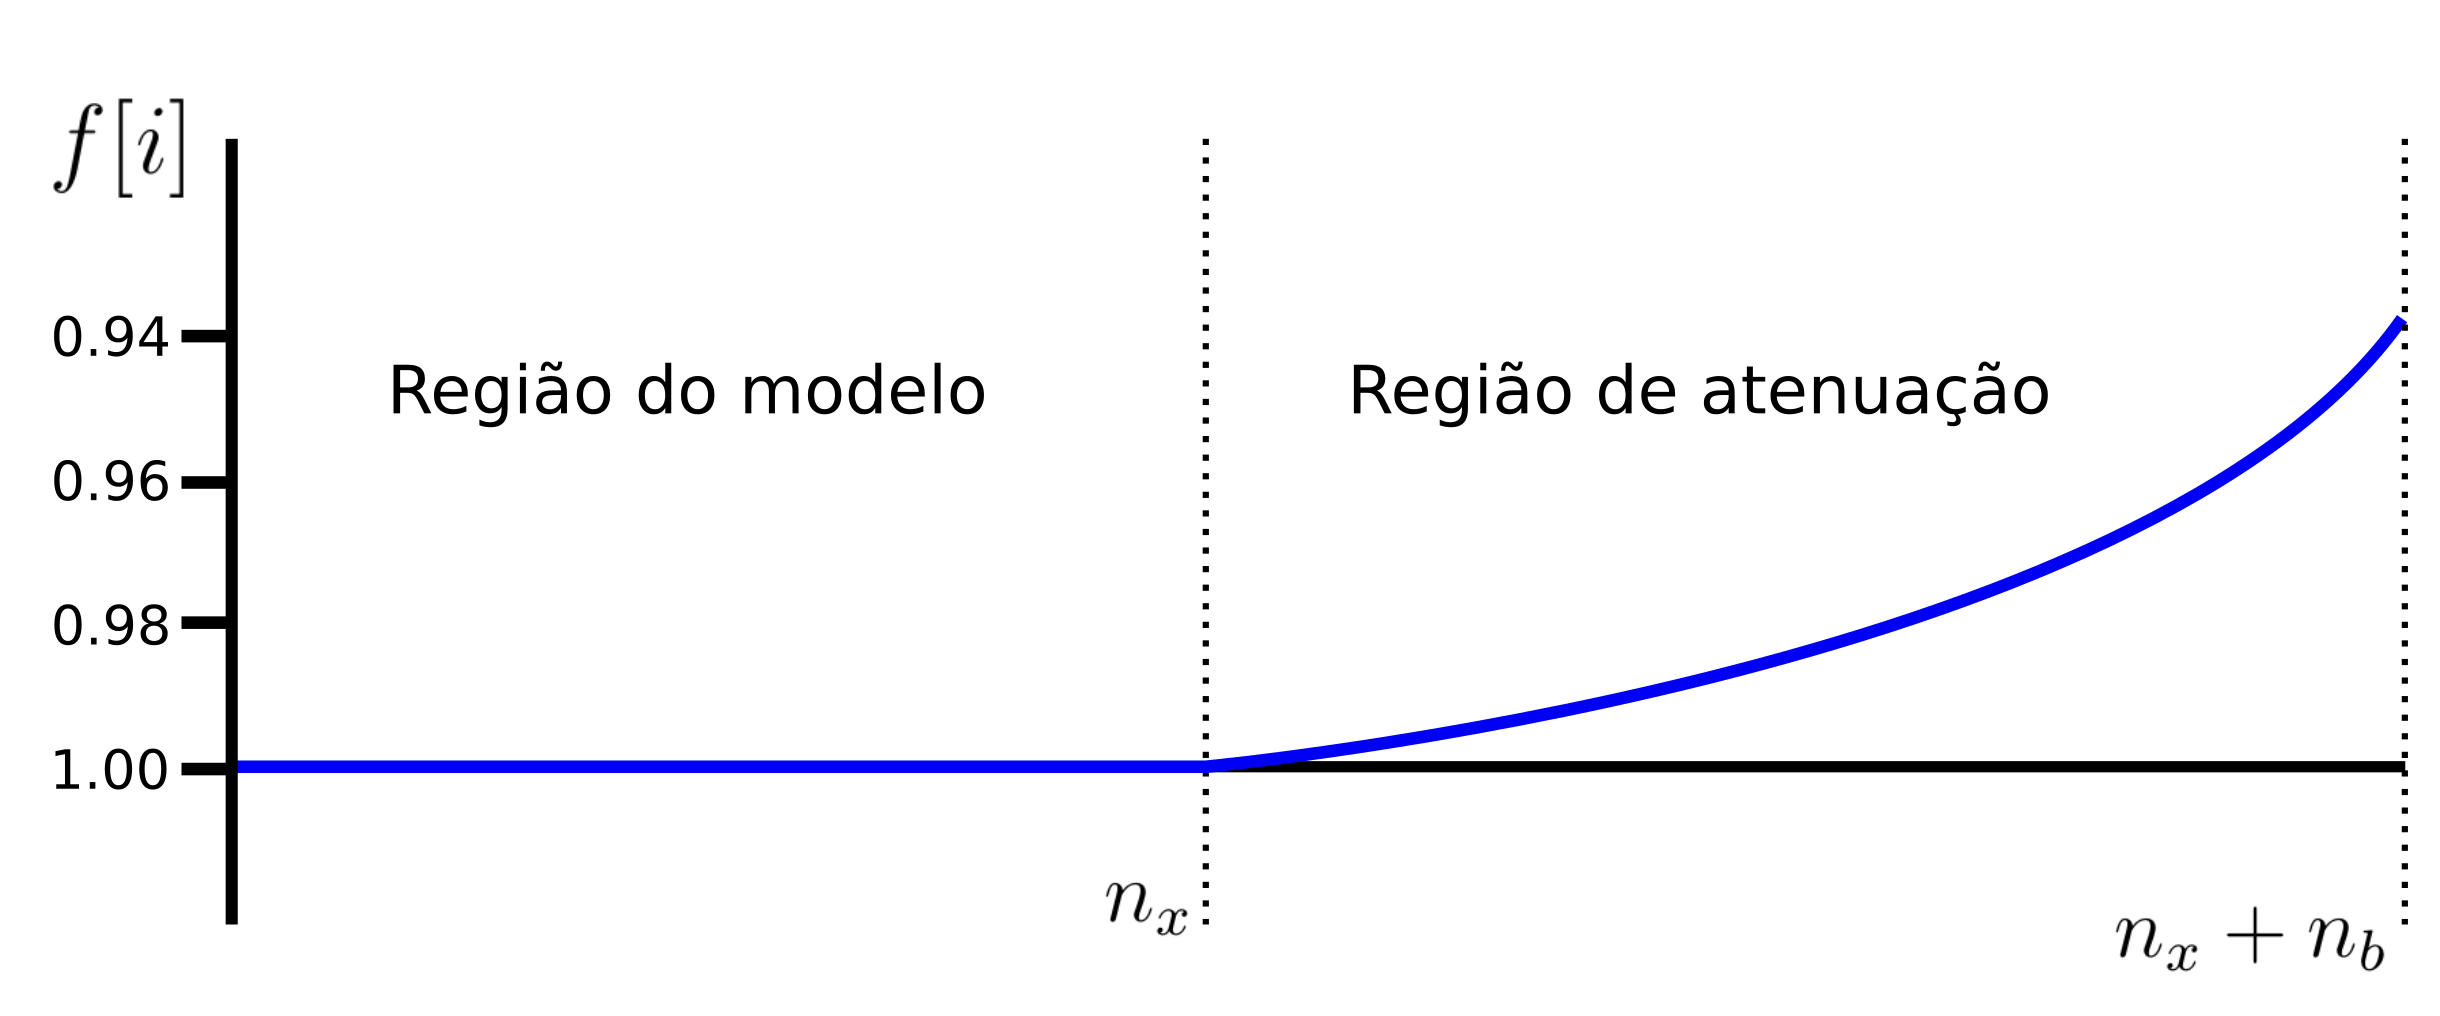
\includegraphics[width=15cm,height=6.5cm]{../imagens/bordas.png}
		\caption{Esquema representando as diferentes regiões no processo de atenuação nas bordas no caso unidimensional. O campo de onda será multiplicado no ponto $nx+i$ pela função $f[i]$ por um valor menor que $1$, diminuindo sua amplitude a cada instante de propagação.}
		\label{damping}
	\end{figure}	 
%	

	Em \citeonline{cerjan1985nonreflecting}, avalia-se valores empíricos de $n_b = 20$ e $\alpha = 0,015$ nos experimentos e, em \citeonline{bording2004finite}, coleta-se os coeficientes otimizados, relacionando custo computacional e eficácia da absorção, sendo eles $n_b = 45$ e $\alpha=0,0053$. No trabalho de  \citeonline{gao2017comparison}, se compara diferentes tipos de equações atenuantes, mostrando que a técnica esponjosa de se retirar energia da onda foi superada pelas novas variantes utilizando modificações da equação da onda para atenuar as energias na borda.  

\subsection*{Aplicação da fonte sísmica}

	As fontes sísmicas mais comuns utilizadas em modelagem de propagação de ondas são as de espectro gaussiano, mais especificamente as fontes derivadas da equação gaussiana. A fonte Ricker, segunda derivada da função gaussiana \cite{ricker1953form}, será usada para gerar os sismogramas sintéticos deste trabalho. 
	
	Particularmente, a aplicação da fonte sísmica em modelagem para meios elásticos de malha intercalada bidimensional tem suas peculiaridades. A primeira delas seria pela natureza da equação de campo duplo, não apresentada aqui, porém amplamente abordada em bibliografias já citadas no inicio deste capítulo. A aplicação da fonte se dá pela derivada, então para visualizar uma Ricker nos campos de onda, deve-se injetar a integral da Ricker nas tensões normais \cite{virieux1986p}. A equação que origina as funções fontes tem a seguinte forma 
%	
	\begin{equation}
		G(t) = \dfrac{A_0}{2\pi(\pi f_c)^2}e^{-\pi(\pi f_c t)^2},
	\end{equation}  
%	
	\noindent sendo $G(t)$ a função gaussiana, $A_0$ um fator de amplitude e $f_c$ um fator que se relaciona com a frequência máxima no espectro gaussiano da seguinte maneira
%	
	\begin{equation}
		f_c = \dfrac{f_{max}}{3\sqrt{\pi}}.
	\end{equation} 	
%	
	\noindent As derivadas de $G(t)$ são dadas pelas seguintes equações 
%	
	\begin{equation}
		\begin{cases}
		G'(t) = - A_0\,t\, e^{-\pi (\pi f_c t)^2} \\
		G''(t) = A_0(1 - 2\pi(\pi f_c t)^2)e^{-\pi (\pi f_c t)^2}, 
		\end{cases}
	\end{equation}	
%	
	\noindent onde $G''(t)$ é a função Ricker e $G'(t)$ sua integral.		
	
	Uma outra peculiaridade para o caso de extrapolação do campo de ondas em duas dimensões seria a forma de onda gerada nos sismogramas sintéticos. O caso 2D é uma aproximação do caso 3D, então, o espalhamento geométrico se torna cilíndrico ao invés de esférico, rotacionando a fase da onda nos sismogramas. No trabalho de \citeonline{pica1990nonlinear}, o problema é resolvido convolvendo os traços dos sismogramas sintéticos por $t^{-\frac{1}{2}}$. Esta correção se mostra computacionalmente custosa já que uma aquisição sintética completa pode possuir um grande número de traços. Aplicando a operação de convolução na fonte sísmica no tempo discreto $t$, os traços se tornam simétricos, porém a transformação foi feita no domínio da frequência angular $w$. 
	
	A correção da fonte será aplicada da seguinte maneira  
%	
	\begin{equation}
		s[t] \,\,\, \xrightarrow{fft}\,\,\, S_c[w] = \sqrt{iw}\,S[w]\,\,\,\xrightarrow{ifft}\,\,\, s_c[t], 
	\end{equation}
%	
	\noindent onde $s_c[n]$ é a fonte corrigida no tempo discreto $t$, $S$ é a função fonte no domínio de Fourier, $S_c$ é a fonte corrigida no domínio da frequência angular $w$, $fft$ e $ifft$ são operações da transformada de Fourier direta e inversa, respectivamente. 
	
	A figura \ref{wavelets}, mostra a sequência de transformações a ser aplicada na fonte antes da modelagem. A figura \ref{modeloTeste}, refere-se ao modelo homogêneo utilizado para o teste da injeção das fontes e a figura \ref{analiseFontes} mostra uma análise das aplicações e seus respectivos resultados. Na prática, se calcula a função Ricker e a integral é calculada numericamente por uma soma amostral, ou seja, cada amostra do resultado recebe a soma das amostras anteriores até a amostra atual da fonte integrada. A correção de fase mostrada anteriormente se aplica no domínio da frequência angular. A ordem das operações não altera o resultado, podendo-se aplicar a correção de fase na fonte Ricker e posteriormente realizar a integração numérica.           	
%	
    \begin{figure}[htp!]
		\centering
		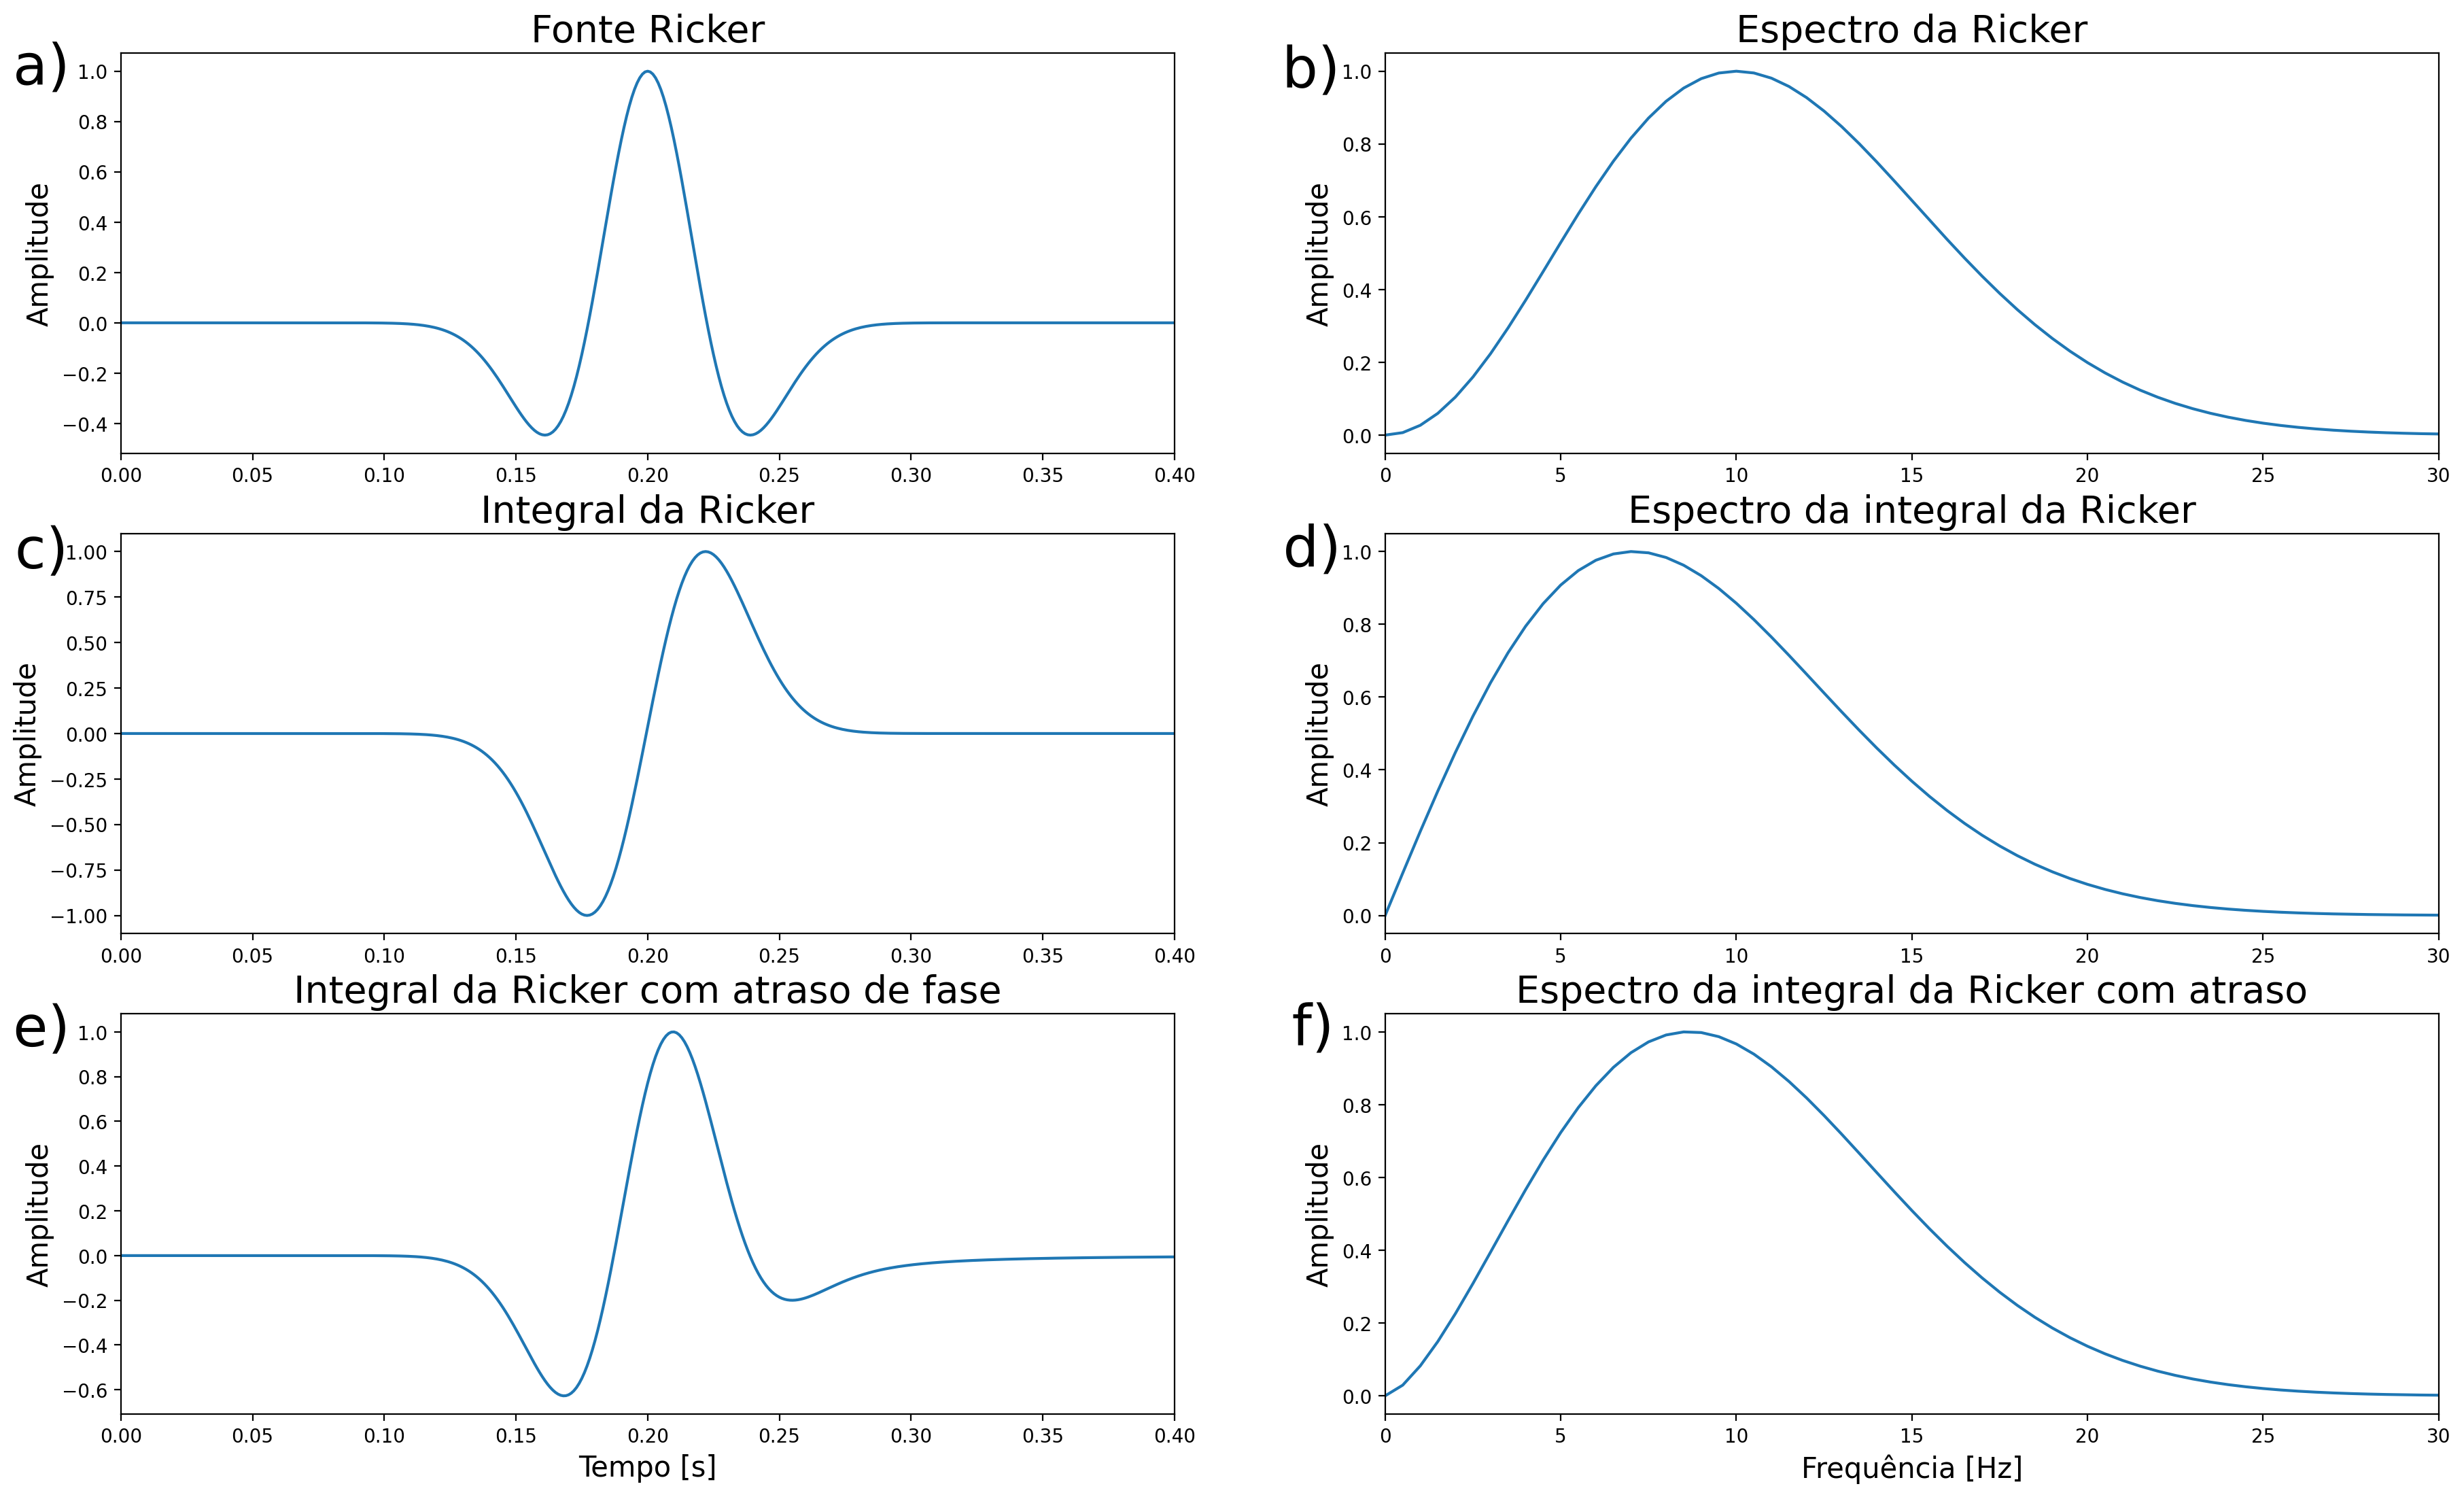
\includegraphics[width=15cm,height=10.5cm]{../imagens/fontes.png}
		\caption{\textbf{a)} Fonte Ricker, \textbf{c)} sua integral e \textbf{e)} fonte resultante após aplicação da correção de fase na integral da Ricker com seus respectivos espectros \textbf{b)}, \textbf{d)} e \textbf{f)}. Existe uma certa alteração na amplitude de acordo com a operação, então todos os gráficos foram normalizados. As fontes tem 400 amostras com parâmetro de discretização de 0,001 segundo, usando uma frequência máxima de 30 Hz.}
		\label{wavelets}
	\end{figure}	 

	Um experimento foi organizado para mostrar a relevância das operações aplicadas de acordo com a geometria da figura \ref{modeloTeste}. A modelagem sísmica simples sem aplicações de bordas absortivas possui modelos com 500 amostras na horizontal e vertical, e 750 amostras no tempo de propagação. Os parâmetros de discretização espacial foi de 5 metros em ambas direções e 1 milissegundo de discretização temporal. A fonte utilizada tem 400 amostras com frequência máxima de 30 Hz sendo aplicada nas tensões normais $\sigma_{xx}$ e $\sigma_{zz}$ disparada no centro do modelo de propriedades. Como resultado, a figura \ref{analiseFontes} mostra os campos de onda de acordo com cada fonte aplicada.
		
	\begin{figure}[htp!]
		\centering
		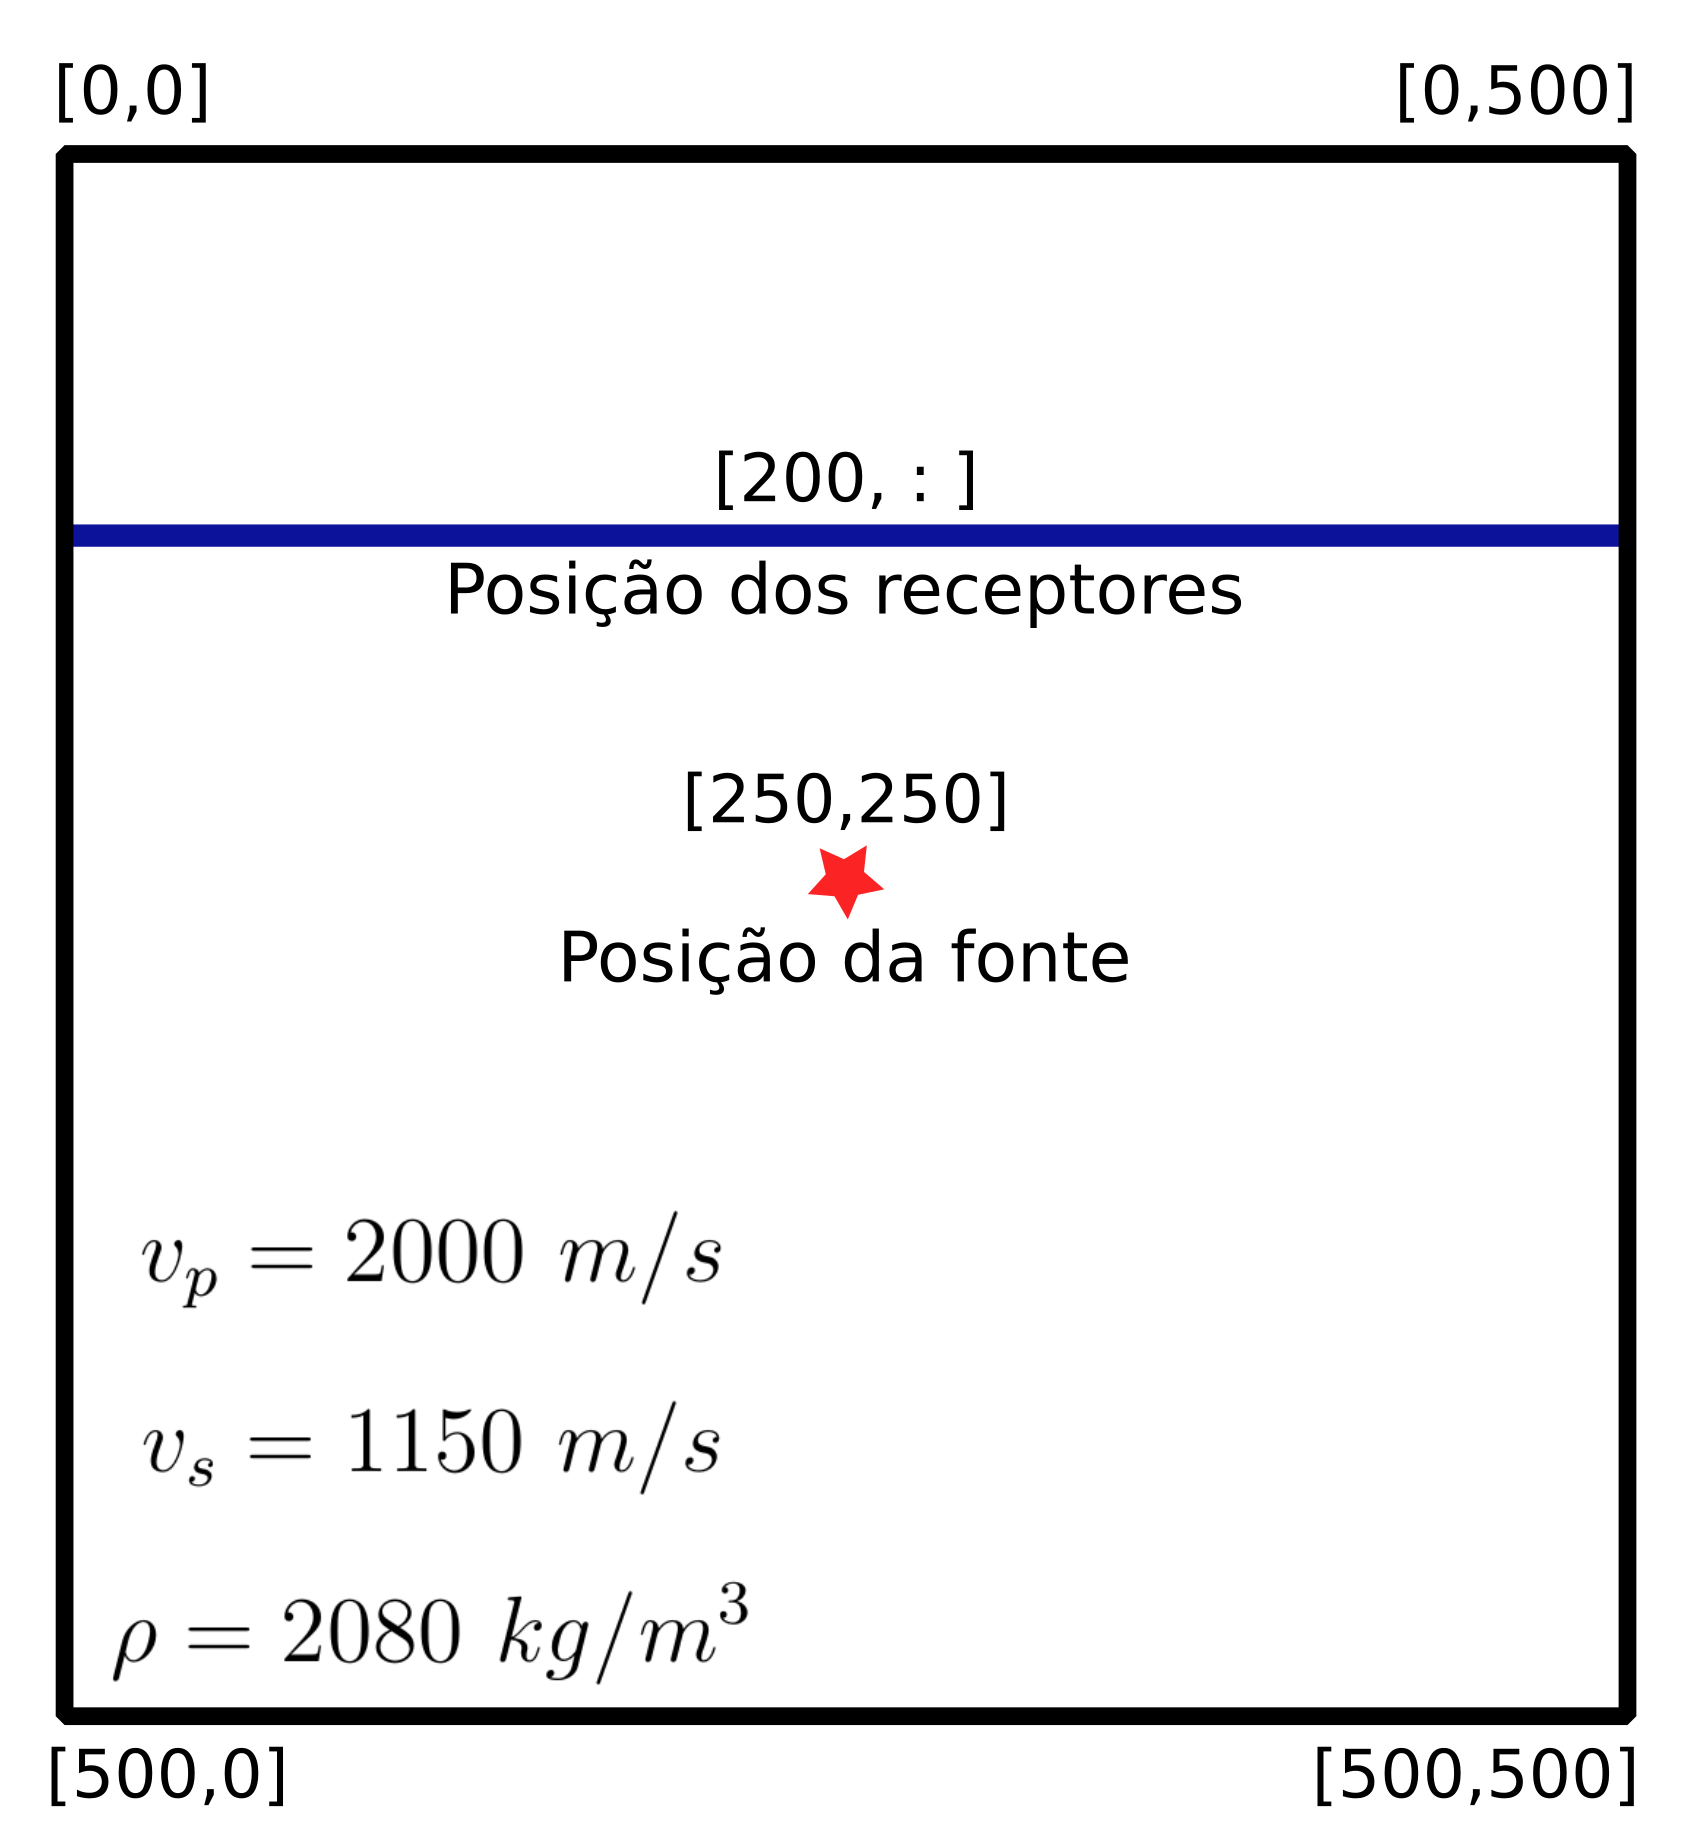
\includegraphics[width=8cm,height=8cm]{../imagens/modeloTeste.png}
		\caption{Modelo de propriedades com geometria de aquisição utilizado para o teste de aplicação da fonte. Ponto de tiro, posição dos receptores, dimensões do modelo e suas propriedades elásticas ilustradas na figura.}
		\label{modeloTeste}
	\end{figure}
%	 	
    \begin{figure}[htp!]
		\centering
		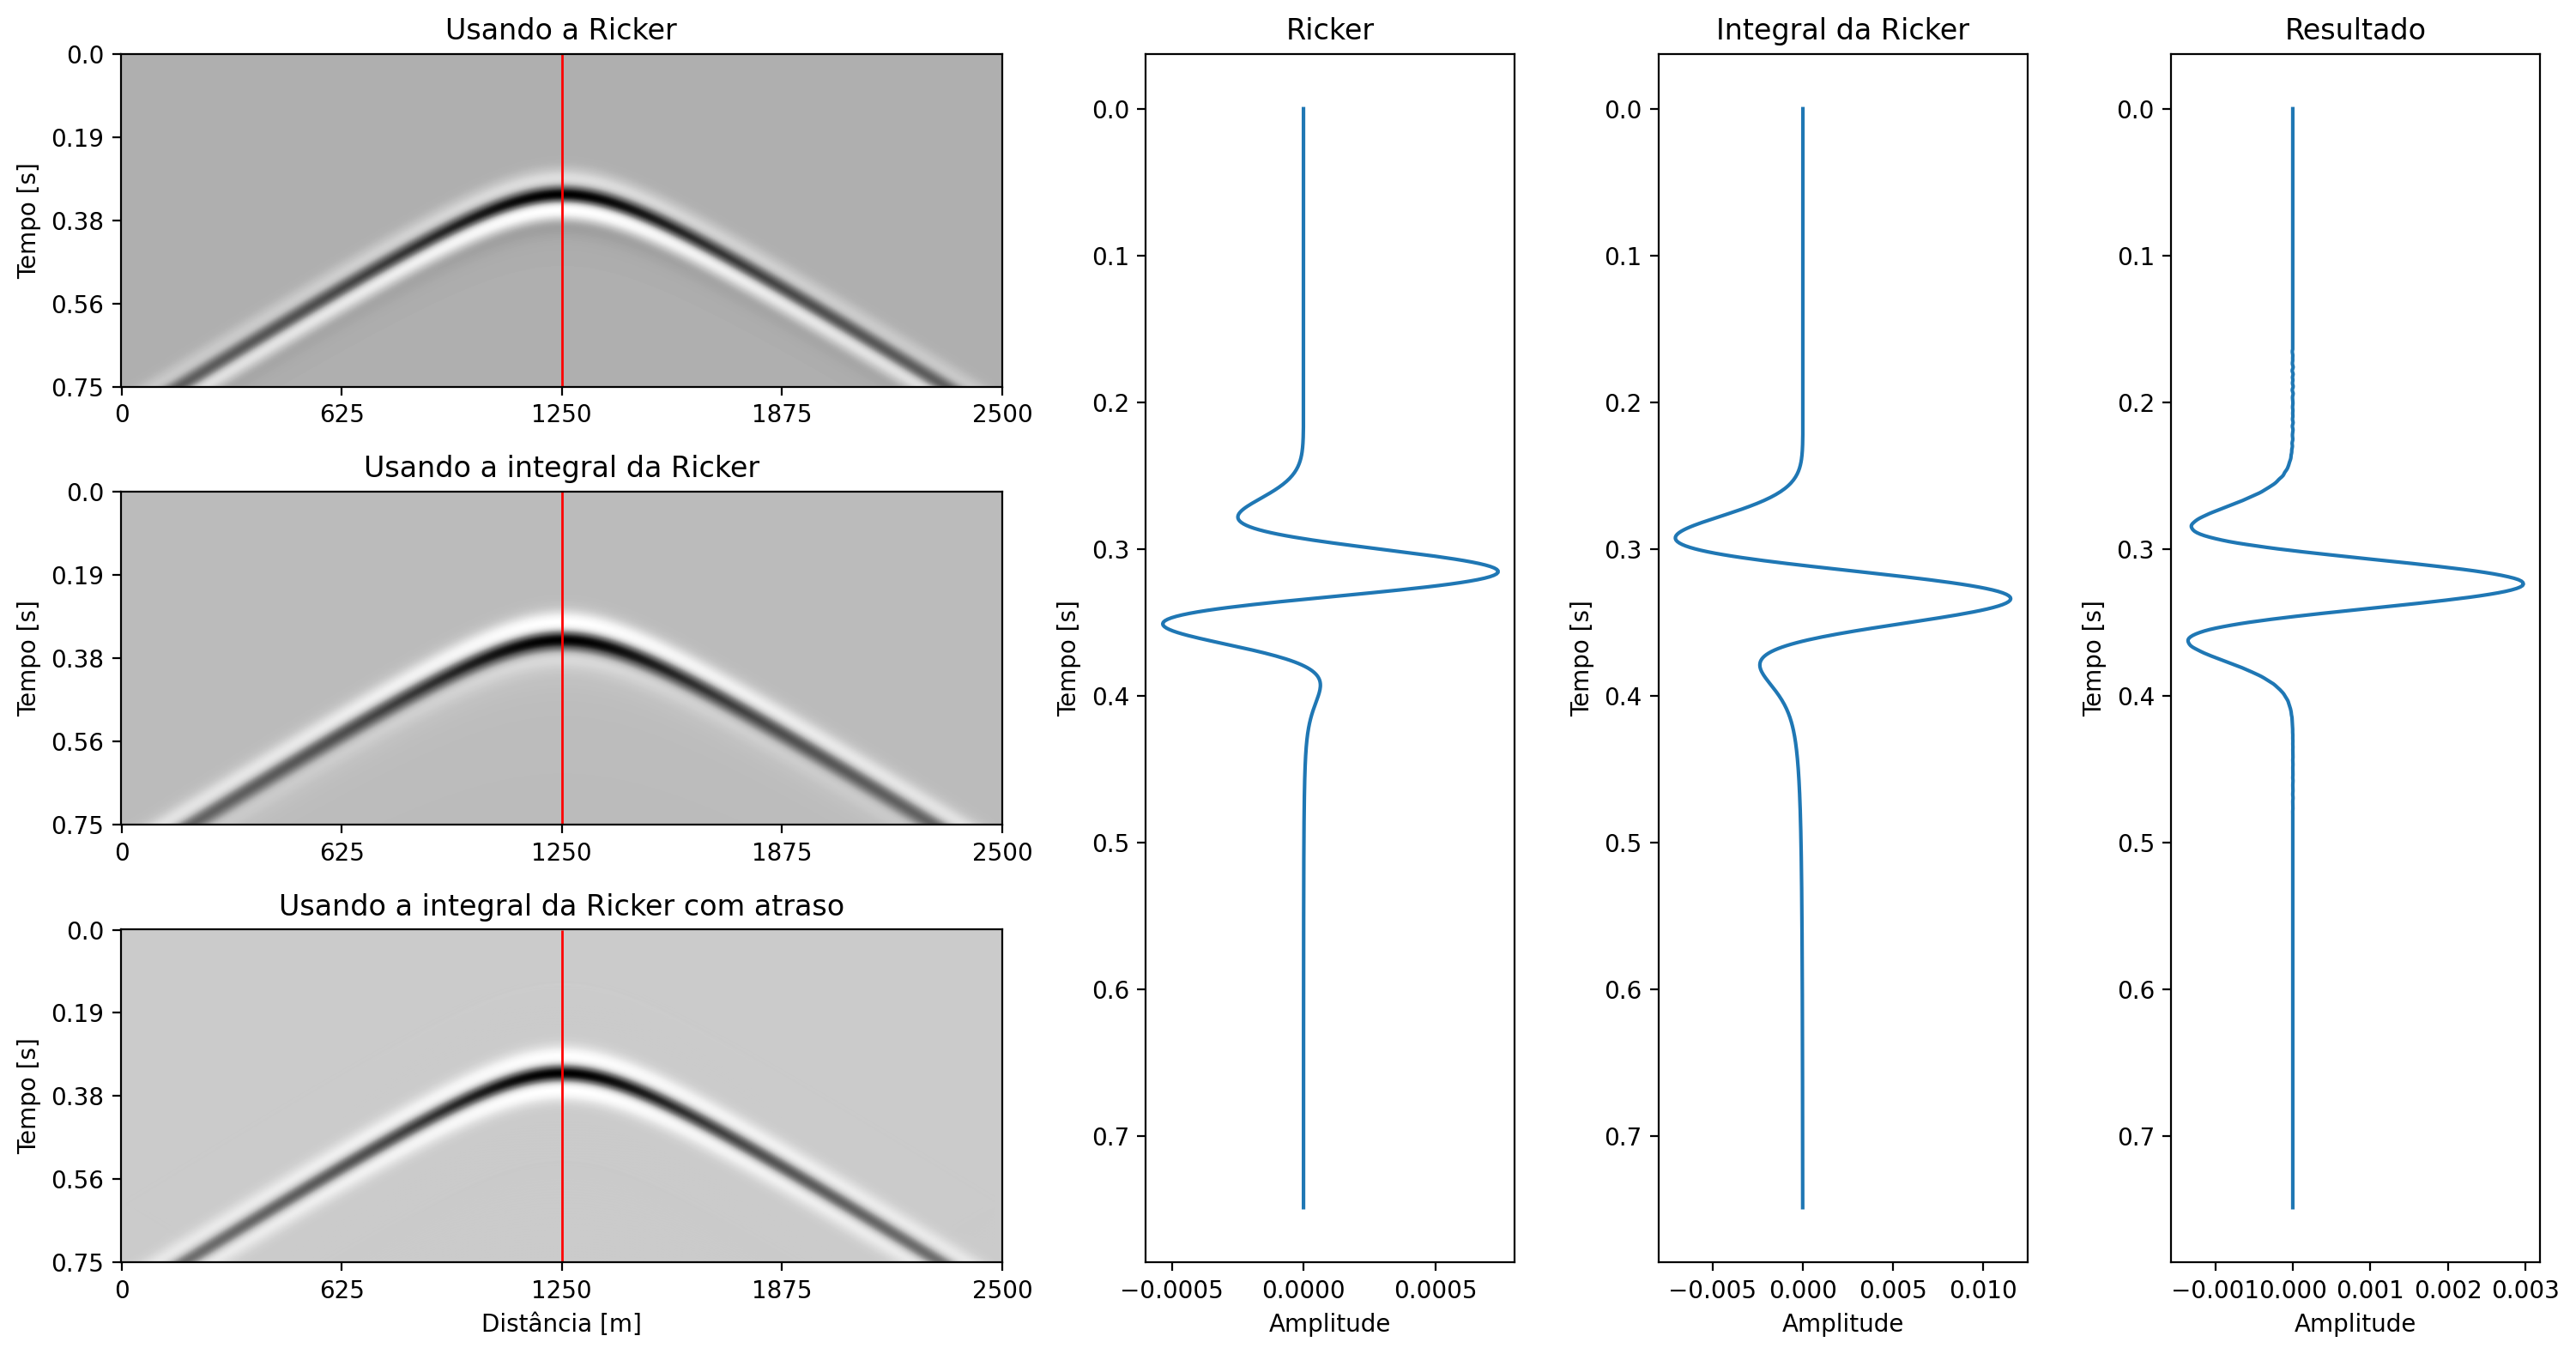
\includegraphics[width=15cm,height=9cm]{../imagens/analiseFontes.png}
		\caption{Experimento realizado para mostrar a relevância da aplicação dos processos na fonte sísmica injetada. Sismogramas coletando a média das tensões normais e cada traço central ilustrando a forma de onda de acordo com a fonte injetada.}
		\label{analiseFontes}
	\end{figure}	  
    
\chapter{Materiais e métodos}

	Este capítulo contempla o material usado e desenvolvido pelo autor para alcançar os resultados. Será apresentado então o dado sísmico utilizado, as modificações realizadas para efetuar o processo de análise das velocidades, todos os detalhes da construção do modelo de propriedades e a aplicação da modelagem sísmica para gerar o dado sintético empilhado. O trabalho foi desenvolvido com programas de código aberto e todos dos processos foram programados pelo autor em ambiente Linux. O \textit{software} livre usado para estimar o campo de velocidades e empilhar os dados real e sintético foi o \textit{Seismic Unix}, baseado nos manuais de \citeonline{stockwell2002new} e \citeonline{forel2005seismic}. As linguagens de programação utilizadas são o python, bash e C, com computação paralela em unidades gráficas de processamento, acelerando os algoritmos em C utilizando \textit{OpenACC} \cite{OpenACC}. Algumas imagens sem citação foram feitas no programa Inkscape e outras utilizando a biblioteca matplotlib do python 3.   

\section{Dado sísmico da margem sudoeste da Inglaterra}
    
    O dado sísmico utilizado neste trabalho foi disponibilizado pelo professor Luiz Alberto Santos (UFF | Petrobras). Esses dados foram obtidos através da \textit{Oil and Gas Authority}, instituição do Reino Unido que trabalha com a indústria e o governo para maximizar o aproveitamento econômico no setor petrolífero e dar suporte para progressiva redução das emissões causadoras do efeito estufa. Contudo, as informações restritas sobre os processos aplicados no dado antes da venda tornam a discussão de alguns aspectos do dado desafiadora. Somente as  informações contidas no cabeçalho do dado (\textit{Header}) foram utilizadas, como dados de localização das fontes/receptores, informações da geometria de aquisição e a própria amplitude do sinal. No total foram três pacotes de dados (Figura \ref{seismEngland}), todos no domínio do ponto médio comum, no formato segy e cada um contendo 3.2 GB de ocupação em disco, sendo eles 
    
    \noindent- MGFLT: Com as reflexões retilíneas, passou por um processo de correção NMO. \newline   
    \noindent- MGRAW: O dado mais bruto do pacote, será usado na análise de velocidades. \newline
    \noindent- PREMIG: Com as refrações suavizadas, seria usado em algum processo de migração.
        
    O dado possui suas coordenadas reais que foram utilizadas para gerar a figura \ref{pontosTiro}. Para melhor entender a geometria de aquisição, o dado foi representado em coordenadas relativas, pois a visualização se torna genérica no espaço, ideal para construção de modelos. 
    
    \newpage
    \noindent As principais informações do dado contidas no \textit{Header} são:
    
    \noindent - Número de tiros: 1604 \newline 
    \noindent - Número de receptores ativos por tiro: 320 \newline
    \noindent - \textit{Offset} mínimo: 100 m \newline
    \noindent - Espaçamento entre receptores e entre disparos: 25 m \newline    
        
    \begin{figure}[htp!]
		\centering
		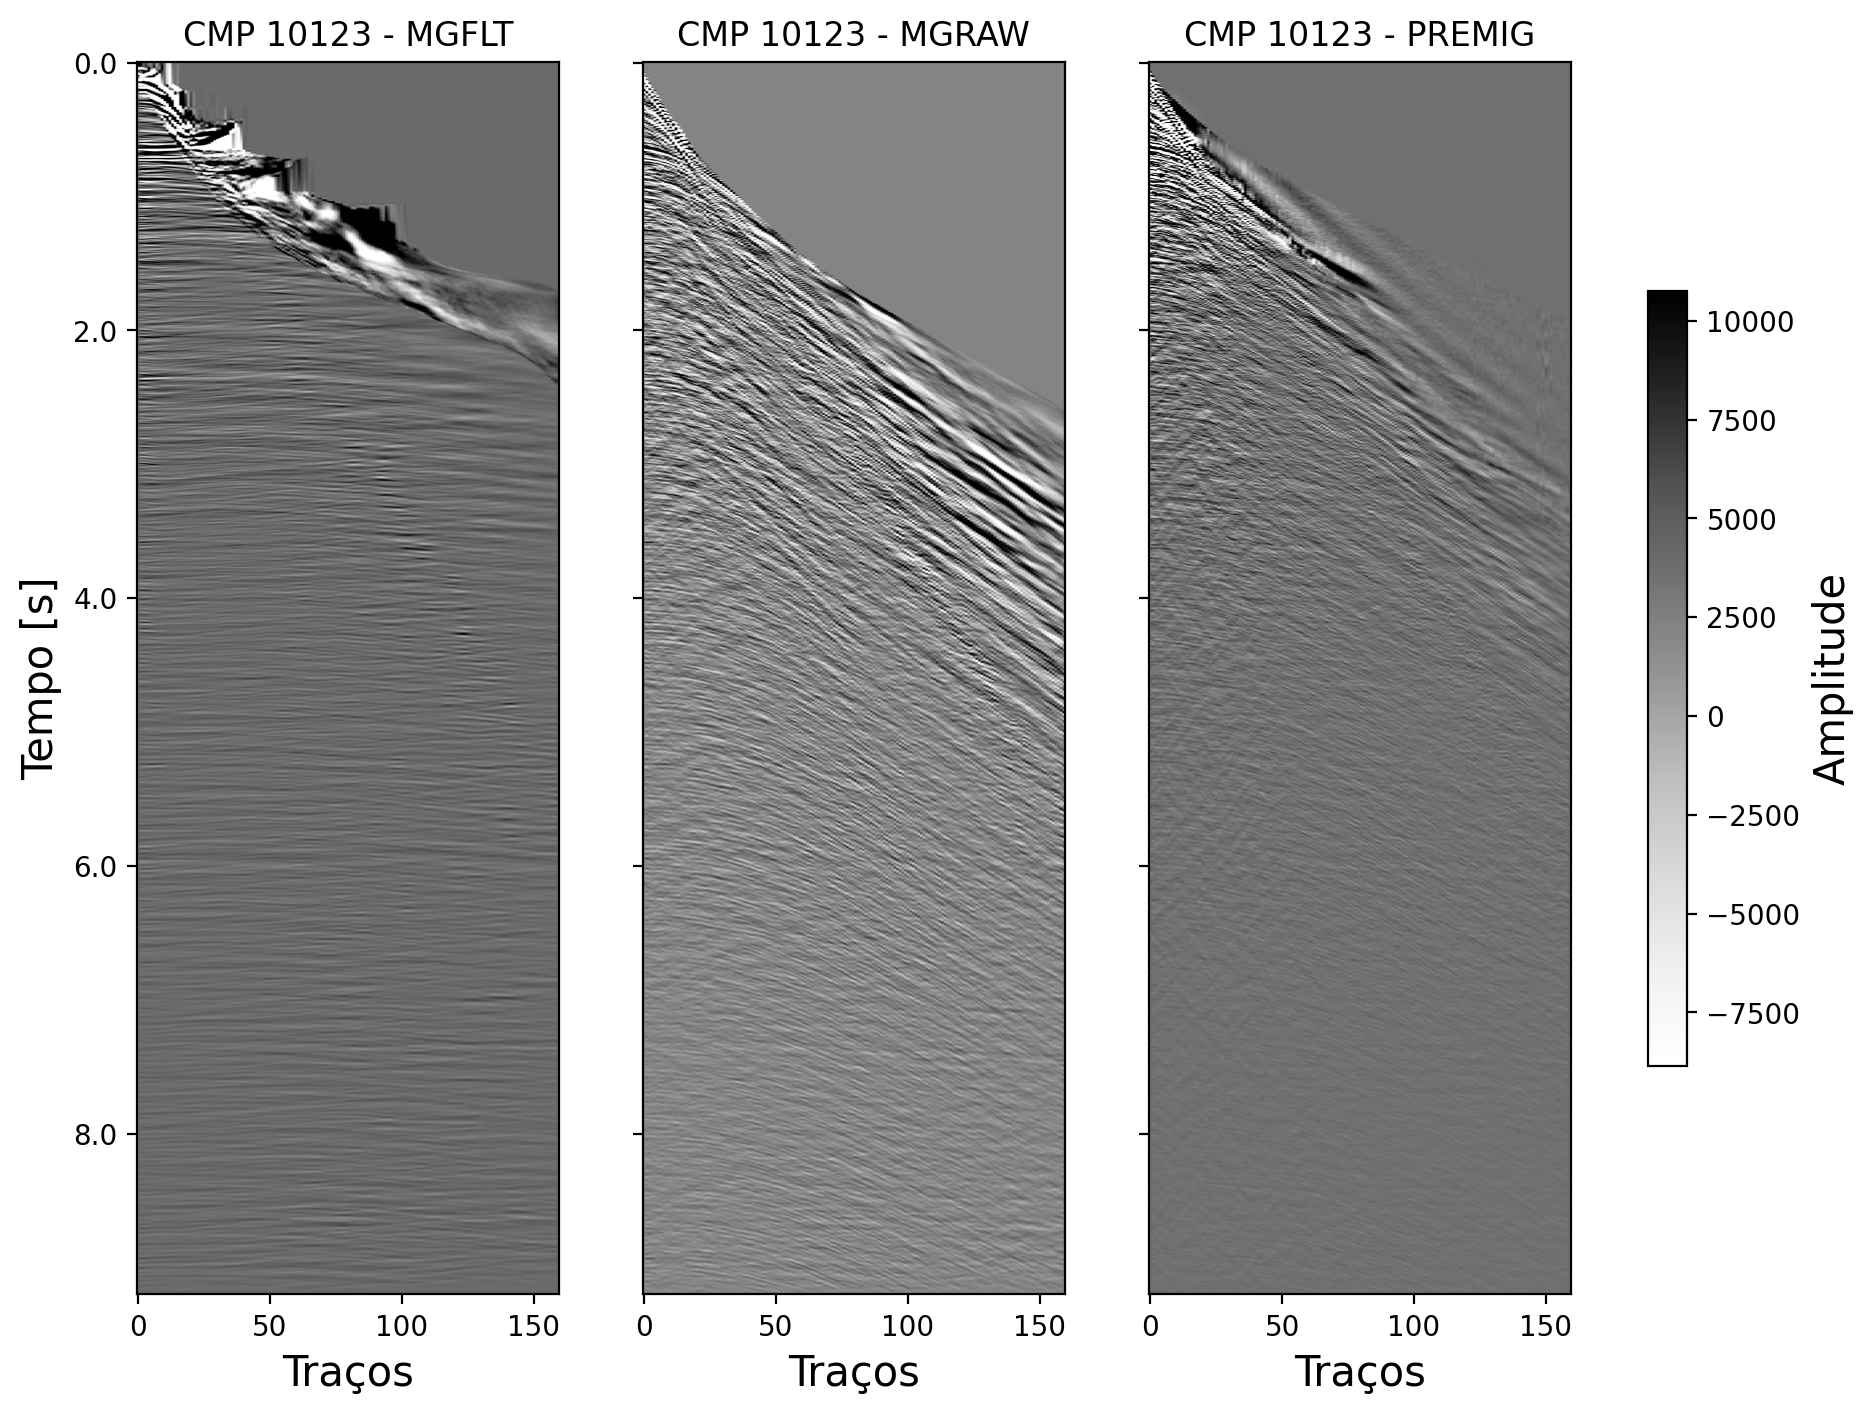
\includegraphics[width=15cm,height=12cm]{../imagens/seismograms.png}
		\caption{Pacote de dados utilizados para a construção do modelo de propriedades elásticas. Cada dado no mesmo CMP contém 160 traços e 9.2 segundos de tempo total.}
		\label{seismEngland}
	\end{figure}
	
	Então, com as principais informações descritas anteriormente, pode-se gerar uma geometria genérica começando do ponto zero e somente variando numa única direção, desenhando uma aquisição bidimensional ideal. A figura \ref{cmpAll}, mostra a geometria genérica completa do dado, que após receber as configurações genéricas, pode ter seus traços reorganizado em qualquer outro domínio além do CMP.  

	Uma forma de avaliar a configuração estrutural da geologia da região seria ordenando os traços no domínio do \textit{offset} comum. Coletando o menor valor de \textit{offset} de todos os pontos de tiro, forma-se uma configuração de aquisição mono canal, onde para cada tiro existe somente um receptor. 
	
	A figura \ref{nearOffset}, mostra a configuração do dado MGRAW no domínio do menor \textit{offset} cortado em 2 segundos, revelando que a partir deste tempo, as amplitudes são aleatórias, não formando feições geológicas. Os dados neste domínio serão usados para estimar a fonte sísmica, ou ao menos o espectro de amplitudes da fonte que gerou os dados. O procedimento se emprega no isolamento da reflexão do fundo marinho de cada traço, soma dos traços e divisão pela quantidade total de traços. 

    \begin{figure}[htp!]
		\centering
		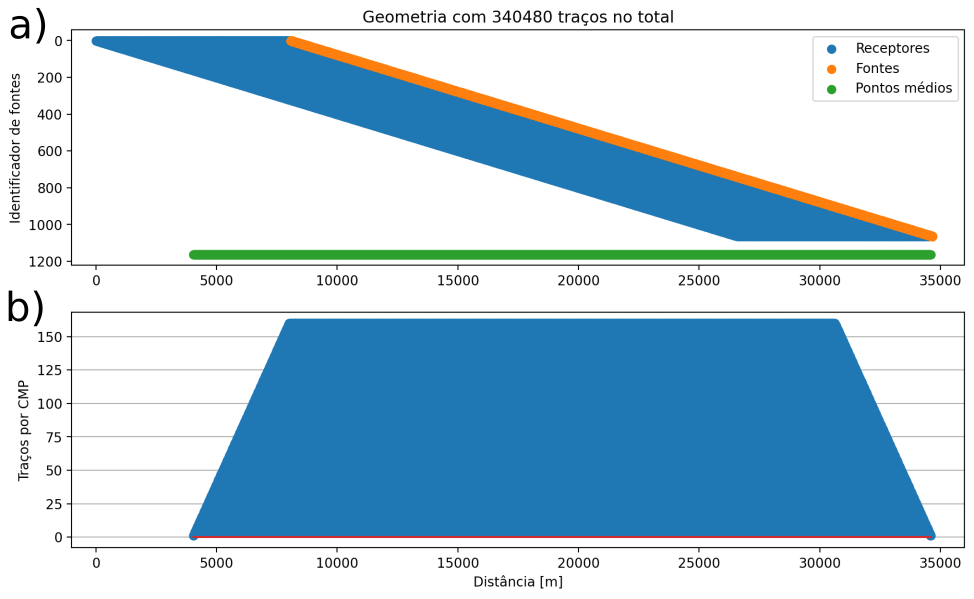
\includegraphics[width=15.5cm,height=12cm]{../imagens/cmpTraceCountAll.png}
		\caption{Geometria genérica que representa a aquisição do dado sísmico da margem sudoeste da Inglaterra. \textbf{a)} Esquema de aquisição se movimentando da esquerda para a direita ilustrando os disparos, receptores e pontos médios. \textbf{b)} traços do esquema para ordenação em CMP é mostrado em relação à distância percorrida no eixo.}
		\label{cmpAll}
	\end{figure}

    \begin{figure}[htp!]
		\centering
		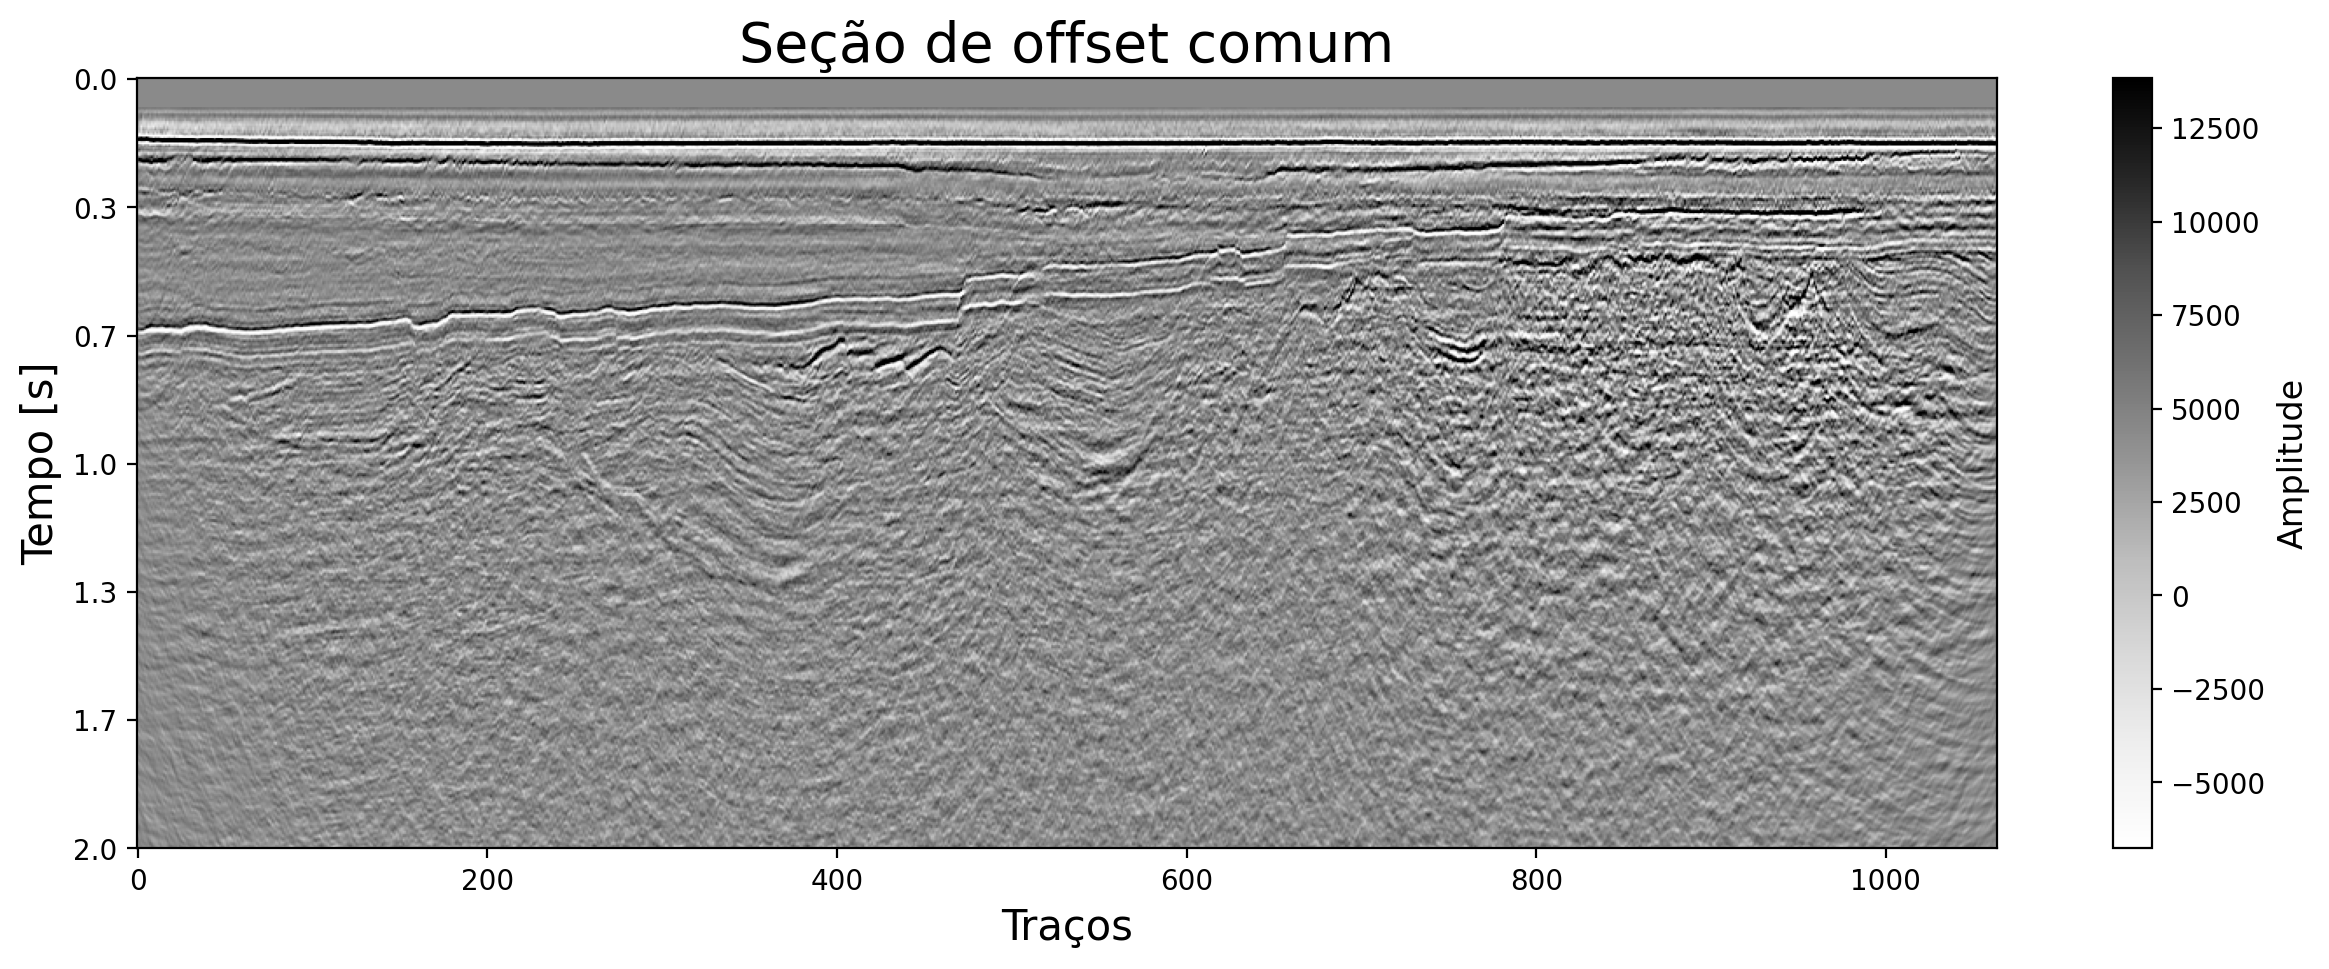
\includegraphics[width=15.5cm,height=7cm]{../imagens/nearOffset.png}
		\caption{Seção de menor \textit{offset} comum. Todos os traços da seção foram coletados no sensor mais próximo da fonte sísmica, sendo o \textit{offset} mínimo de 100 metros e o espaçamento entre disparos de 25 metros.}
		\label{nearOffset}
	\end{figure}

\section{Construção do modelo de velocidades}

	O método da sísmica de reflexão busca registrar a iluminação de um ponto por uma onda em subsuperfície o máximo de vezes possível. Essas posições em profundidade, projetadas na superfície, são parte da família de pontos médios comuns, que são localizados entre uma fonte e um receptor numa aquisição sísmica. A técnica de análise de velocidades é aplicada somente onde a aquisição sísmica tem a maior varredura desses pontos médios, ou seja, quando o número de traços que ilumina o ponto médio é máximo. Na figura \ref{cmpFullFold}, é mostrada a geometria de aquisição e a taxa de iluminação dos pontos médios comuns. Nessa região em específico, será estimado o modelo de velocidades e contemplará o dado empilhado.     				

    \begin{figure}[htp!]
		\centering
		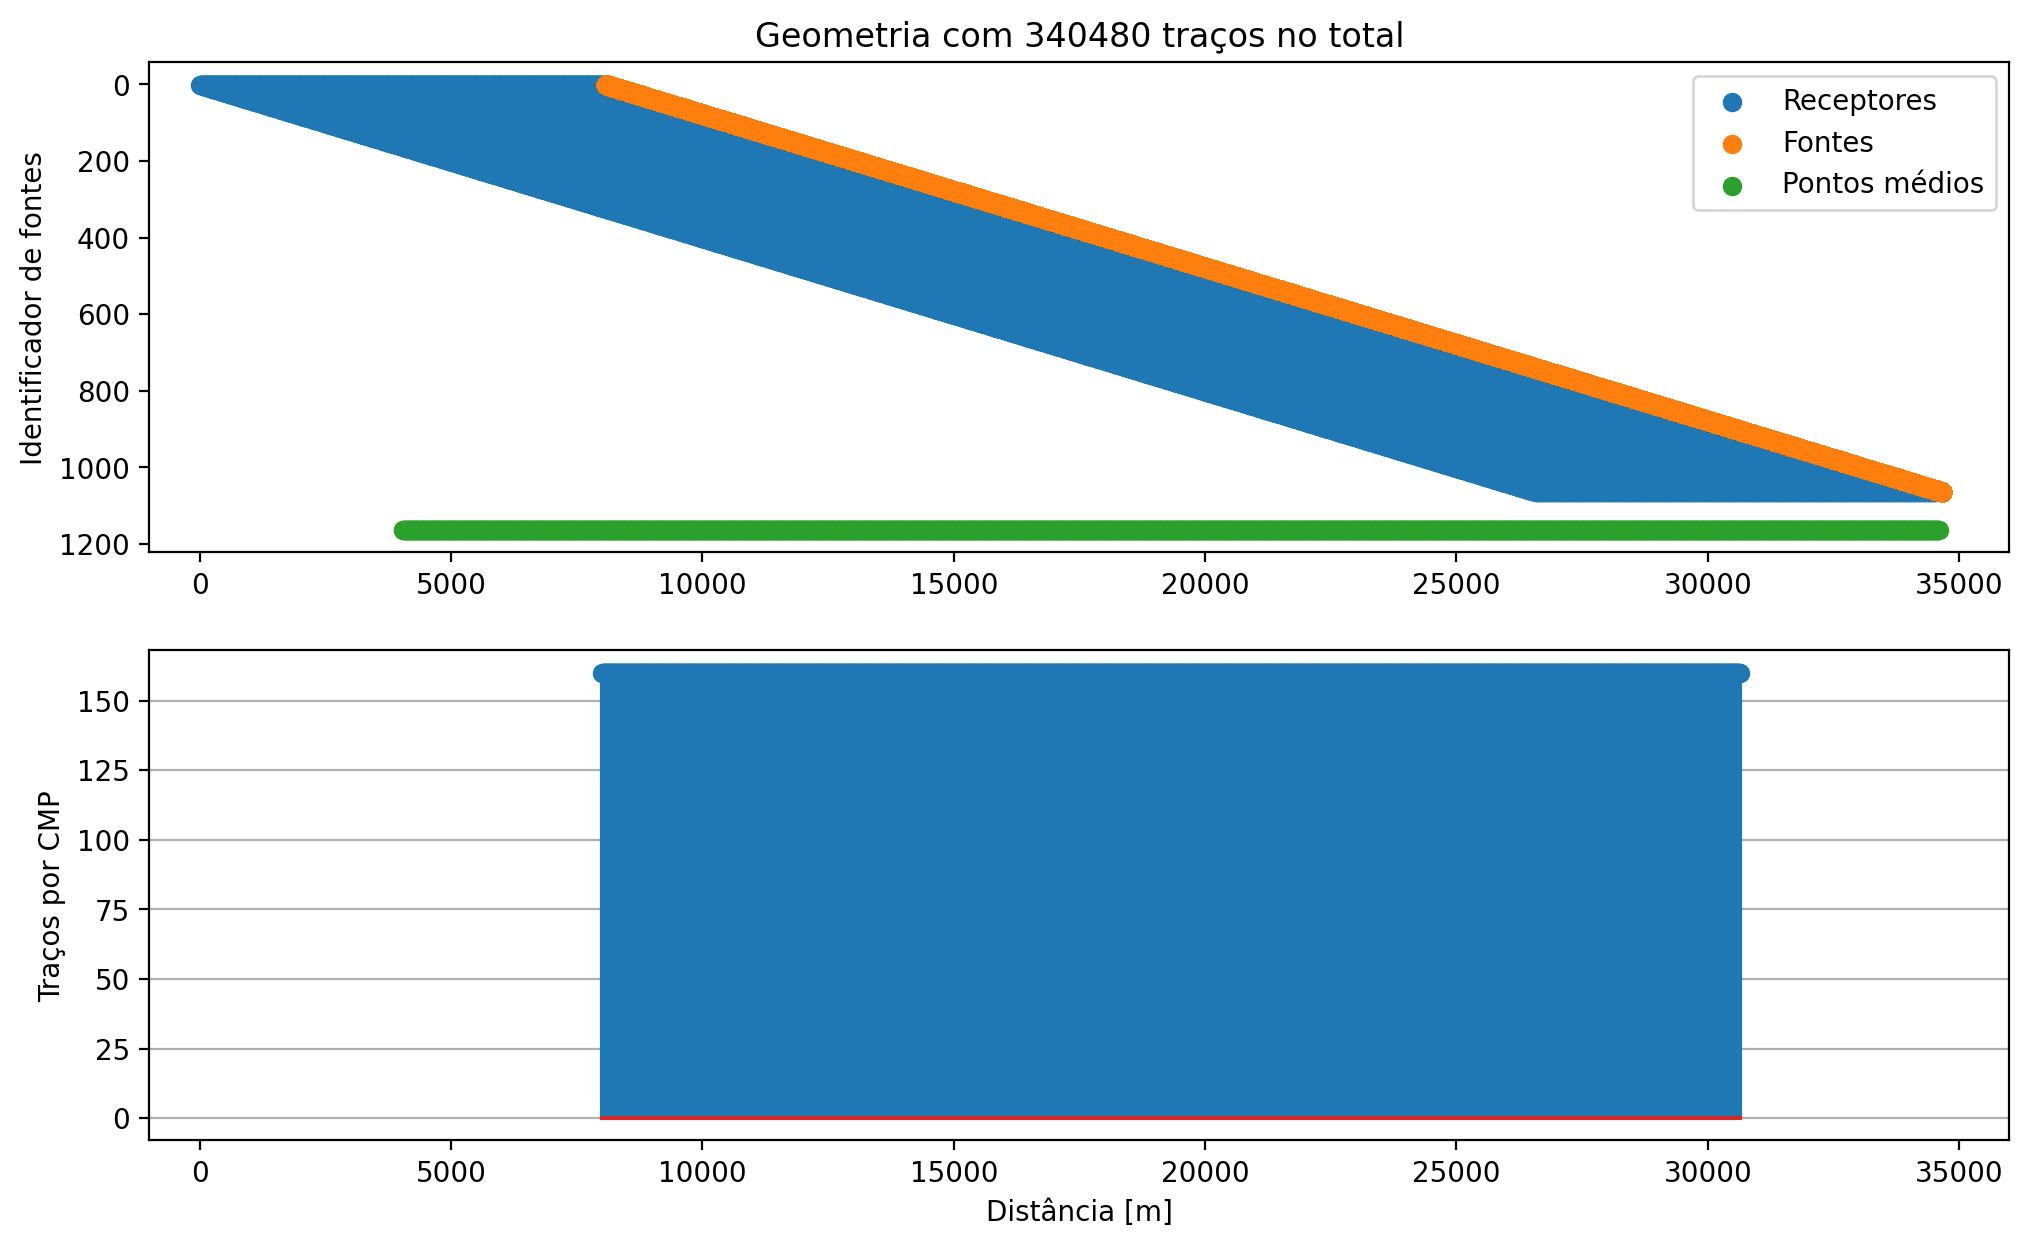
\includegraphics[width=16cm,height=11cm]{../imagens/cmpTraceCountFullFold.png}
		\caption{Esquema de geometria explicitando as posições dos pontos médios comum de máxima varredura na aquisição sísmica. Cada sismograma de ponto médio com varredura completa contém 160 traços.}
		\label{cmpFullFold}
	\end{figure}
	
	A aquisição possui 1810 pontos médios comuns com máxima varredura de traços espaçados de 12,5 metros no espaço, abrangendo uma extensão de 22625 metros. Nesse intervalo foi escolhido, através de um espaçamento regular de 180 CMPs, 11 sismogramas no total para serem analisados, como mostrado na figura \ref{cmpVelAn}. O código utilizado para realizar a análise de velocidades está disponível em \citeonline{forel2005seismic}, chamado \textit{IVA - Interactive Velocity Analysis}, onde se aplica iterativamente o processo de análise de velocidades para um grupo de sismogramas CMP pré-determinado.         
	
    \begin{figure}[htp!]
		\centering
		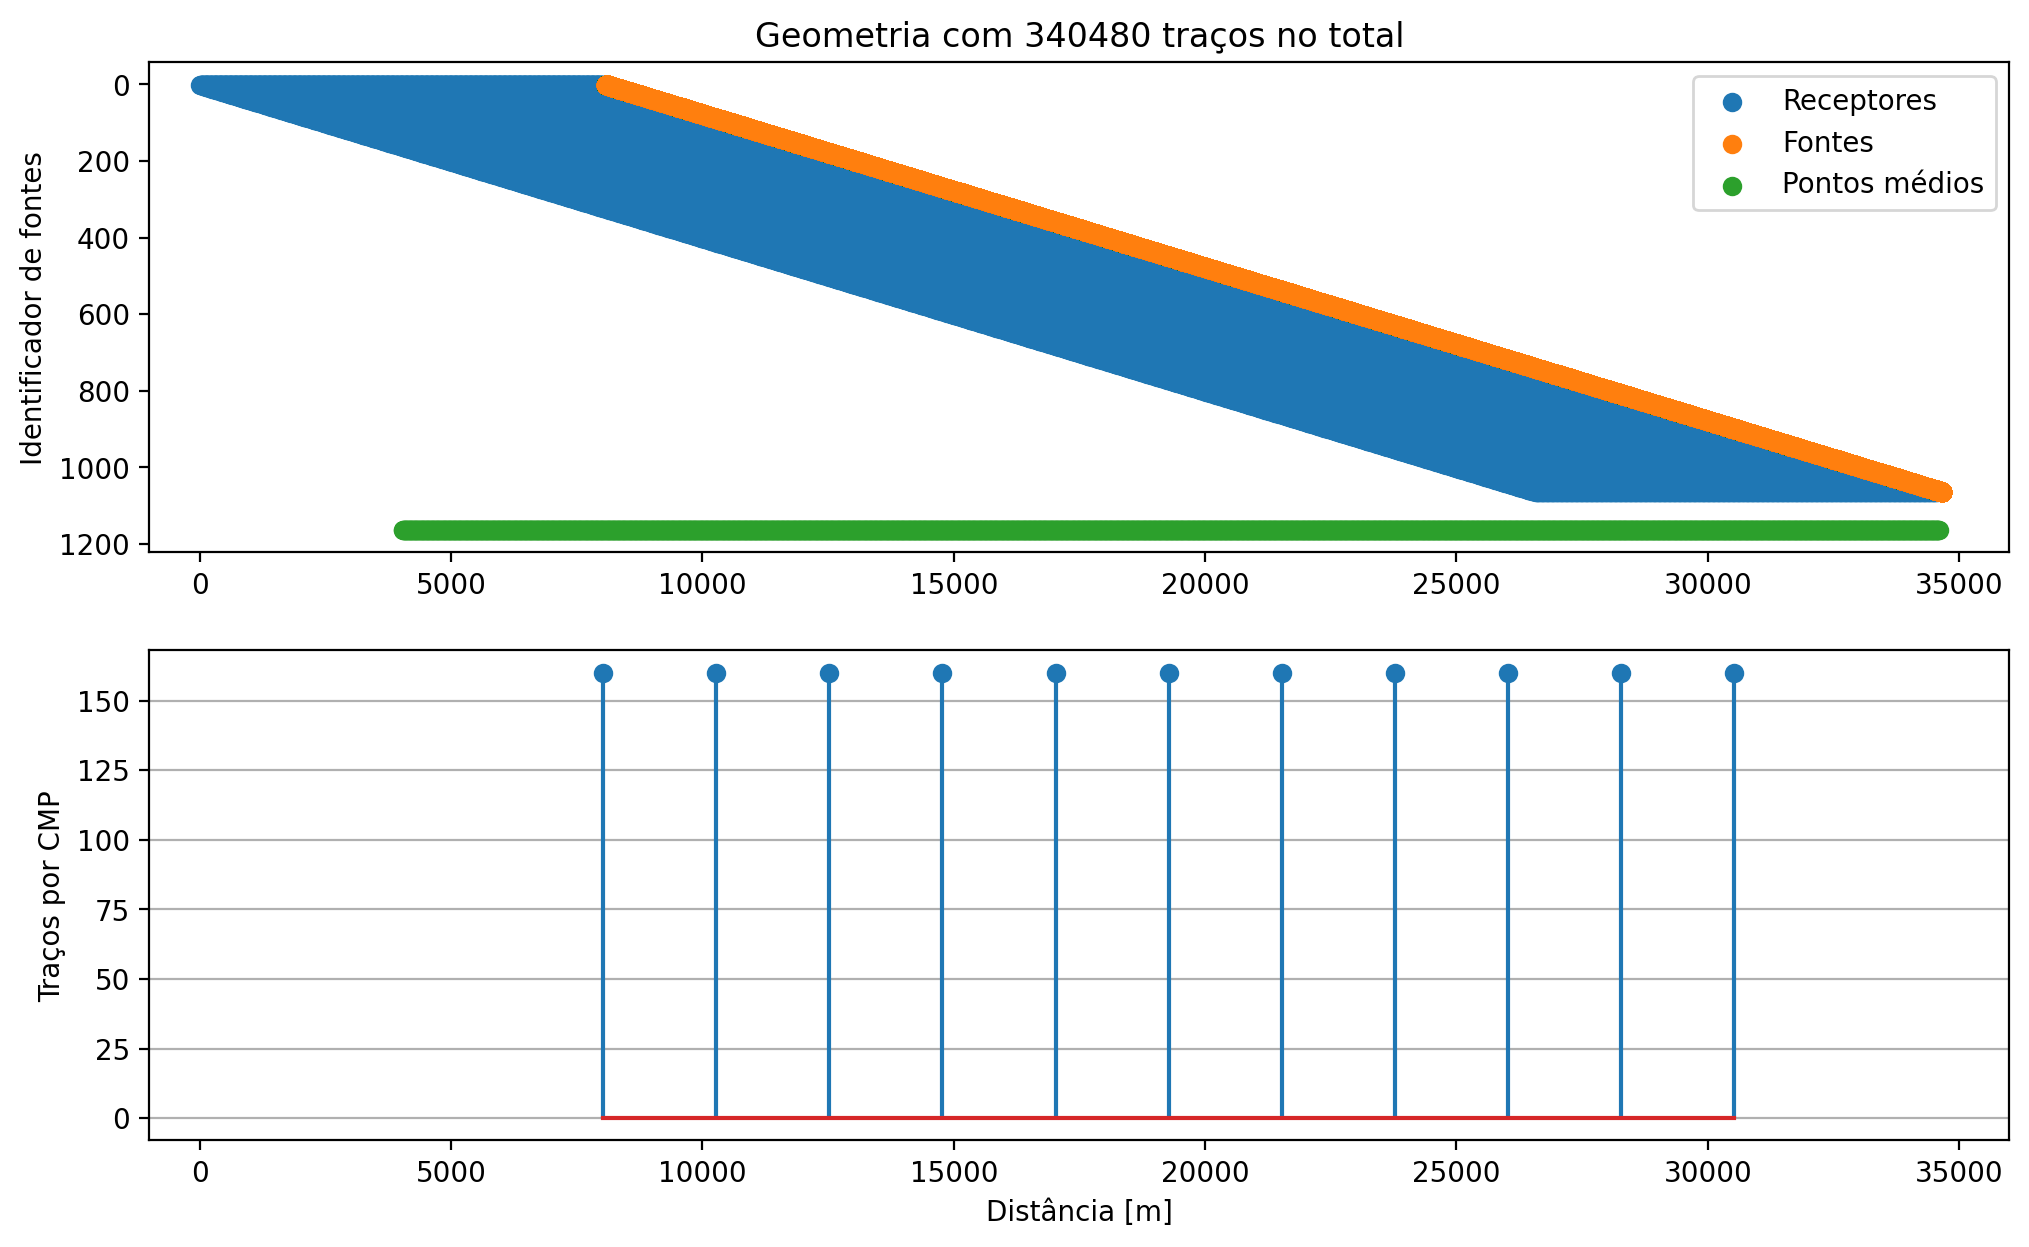
\includegraphics[width=16cm,height=12cm]{../imagens/cmpTraceCountVelAn.png}
		\caption{Seleção das posições coletadas para a realização do processo de análise de velocidades. CMPs espaçados de 2250 metros para gerar um modelo suave.}
		\label{cmpVelAn}
	\end{figure}

	O processo de análise de velocidades se resume em coletar tempo e velocidade que melhor ajustam a reflexão no sismograma CMP utilizando a equação \ref{velan}. O \textit{semblance} correlaciona o tempo e velocidade mais provável que representa a hipérbole de reflexão no sismograma CMP. A figura \ref{realProc}, mostra um exemplo do processo. 

	Primeiro, se escolhe um sismograma contendo a máxima varredura de traços, pois assim as informações das reflexões serão completas, ou seja, as hipérboles tem mais pontos por reflexão (maior \textit{move out}). Posteriormente, a matriz de correlação mostrará pontos de tempo e velocidade a serem escolhidos, sendo que a velocidade em questão pode ser aproximada pela média quadrática da velocidade do meio - velocidade RMS. 
	
	Em seguida, a correção \textit{normal move out} é aplicada no sismograma, horizontalizando as reflexões e silenciando os traços com \textit{offset} longo, reduzindo o efeito do \textit{stretching} (estiramentos nas hipérboles de reflexão que se tornam ruídos após a correção NMO). 
	
	E por fim, o sismograma corrigido é empilhado somando todas as amostras dos traços lateralmente, obtendo um único traço. A seção empilhada será a sucessão de traços empilhados na posição onde os sismogramas CMP de varredura completa se encontram na geometria de aquisição. 

    \begin{figure}[htp!]
		\centering
		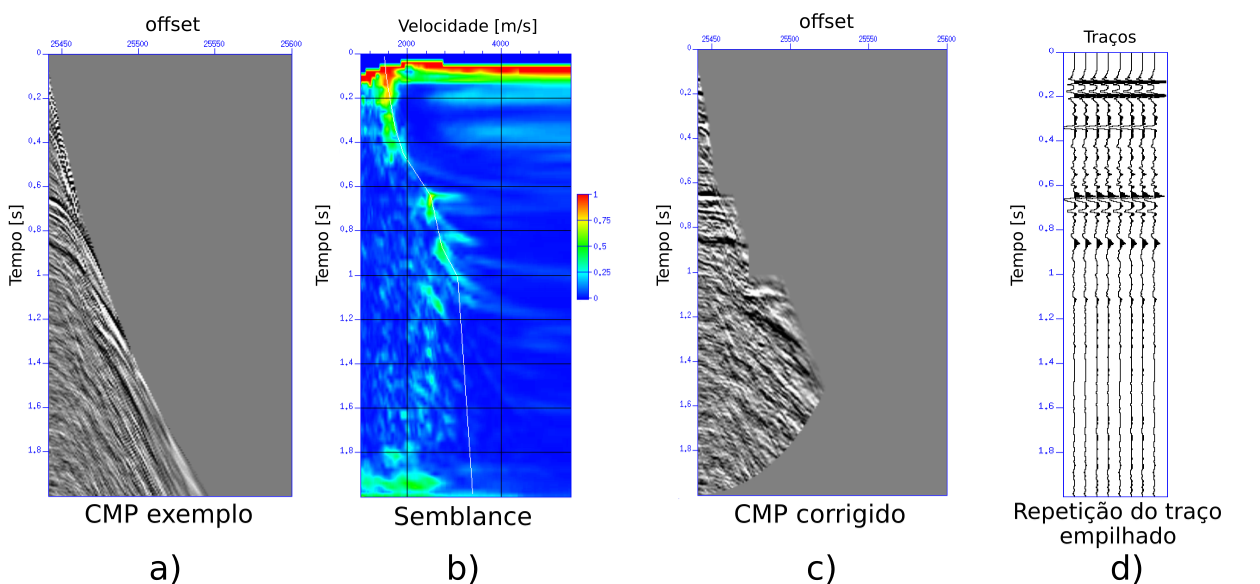
\includegraphics[width=16cm,height=8cm]{../imagens/processamentoReal.png}
		\caption{Estimativa de velocidade num sismograma CMP de varredura completa. Apresentação da matriz que correlaciona o tempo e velocidade RMS com a função de velocidades que melhor ajustaria os dados. Dado com NMO corrigido e a repetição do traço empilhado também mostrados.}
		\label{realProc}
	\end{figure}

	O programa de análise de velocidades exporta um arquivo contendo os tempos e as velocidades coletadas a partir do painel da matriz de correlação \textit{semblance}. Todo o esquema de construção do modelo de velocidades foi implementado em python, sendo que o primeiro passo foi ler o arquivo exportado pelo algoritmo de análise iterativa de velocidades. A figura \ref{picks} mostra, os \textit{picks} de velocidade por CMP analisado, que são as velocidades RMS coletadas analisando os sismogramas CMP pré-estabelecidos.
	
    \begin{figure}[htp!]
		\centering
		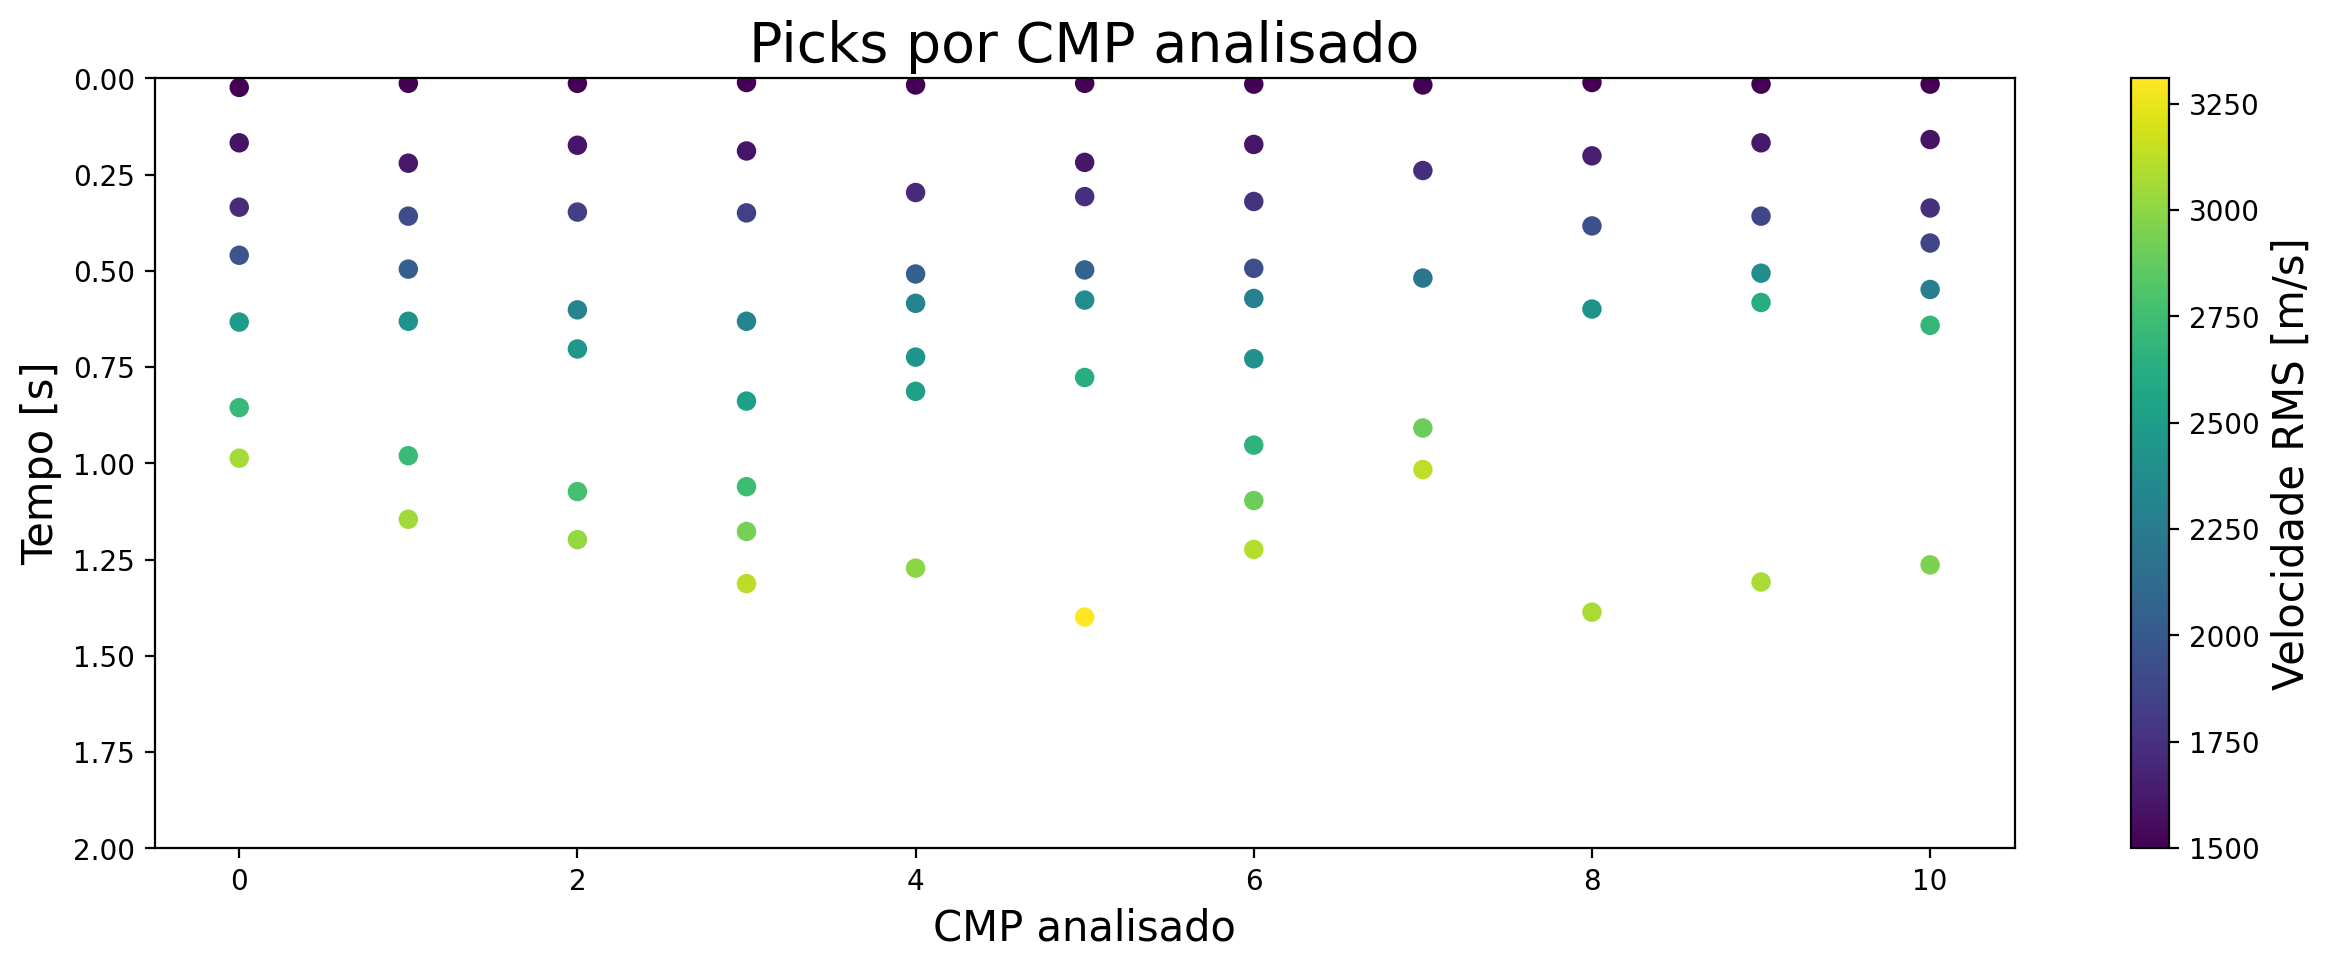
\includegraphics[width=16cm,height=7.5cm]{../imagens/picksFocado.png}
		\caption{Velocidades RMS estimadas a partir do método da análise de velocidades. Foi realizada uma leitura do arquivo exportado pelo algoritmo análise iterativa.}
		\label{picks}
	\end{figure}
	
	Os pontos de velocidade tem dimensão de tempo e CMP analisado, onde estão dispostos irregularmente no tempo. Para o início da geração do modelo de velocidades, foi implementado um algoritmo de interpolação linear irregular no tempo, aplicado em cada \textit{array} de velocidade (figura \ref{picksVertInterp}). Para encontrar o tamanho dos \textit{arrays} no domínio do tempo, foi utilizada a informação da discretização temporal do dado sísmico de 4 $ms$. 
	
	Em \textit{arrays} de 2 segundos no total, foram precisas 501 amostras para realizar a interpolação linear irregular. Um fator a ser considerado foi que a amostra inicial e final dos \textit{arrays} estavam sem valor de velocidade, então as velocidades RMS de 1490 $m/s$ e 4000 $m/s$ foram aplicadas no início e final dos \textit{arrays} respectivamente a fim de pré-condicionar a interpolação linear irregular. A algoritmo interpolador funciona basicamente vasculhando as amostras sem valor, guardando as velocidades próximas naquele intervalo sem valor e adicionando uma média ponderada de velocidade de acordo com a quantidade de amostras.    
%
    \begin{figure}[htp!]
		\centering
		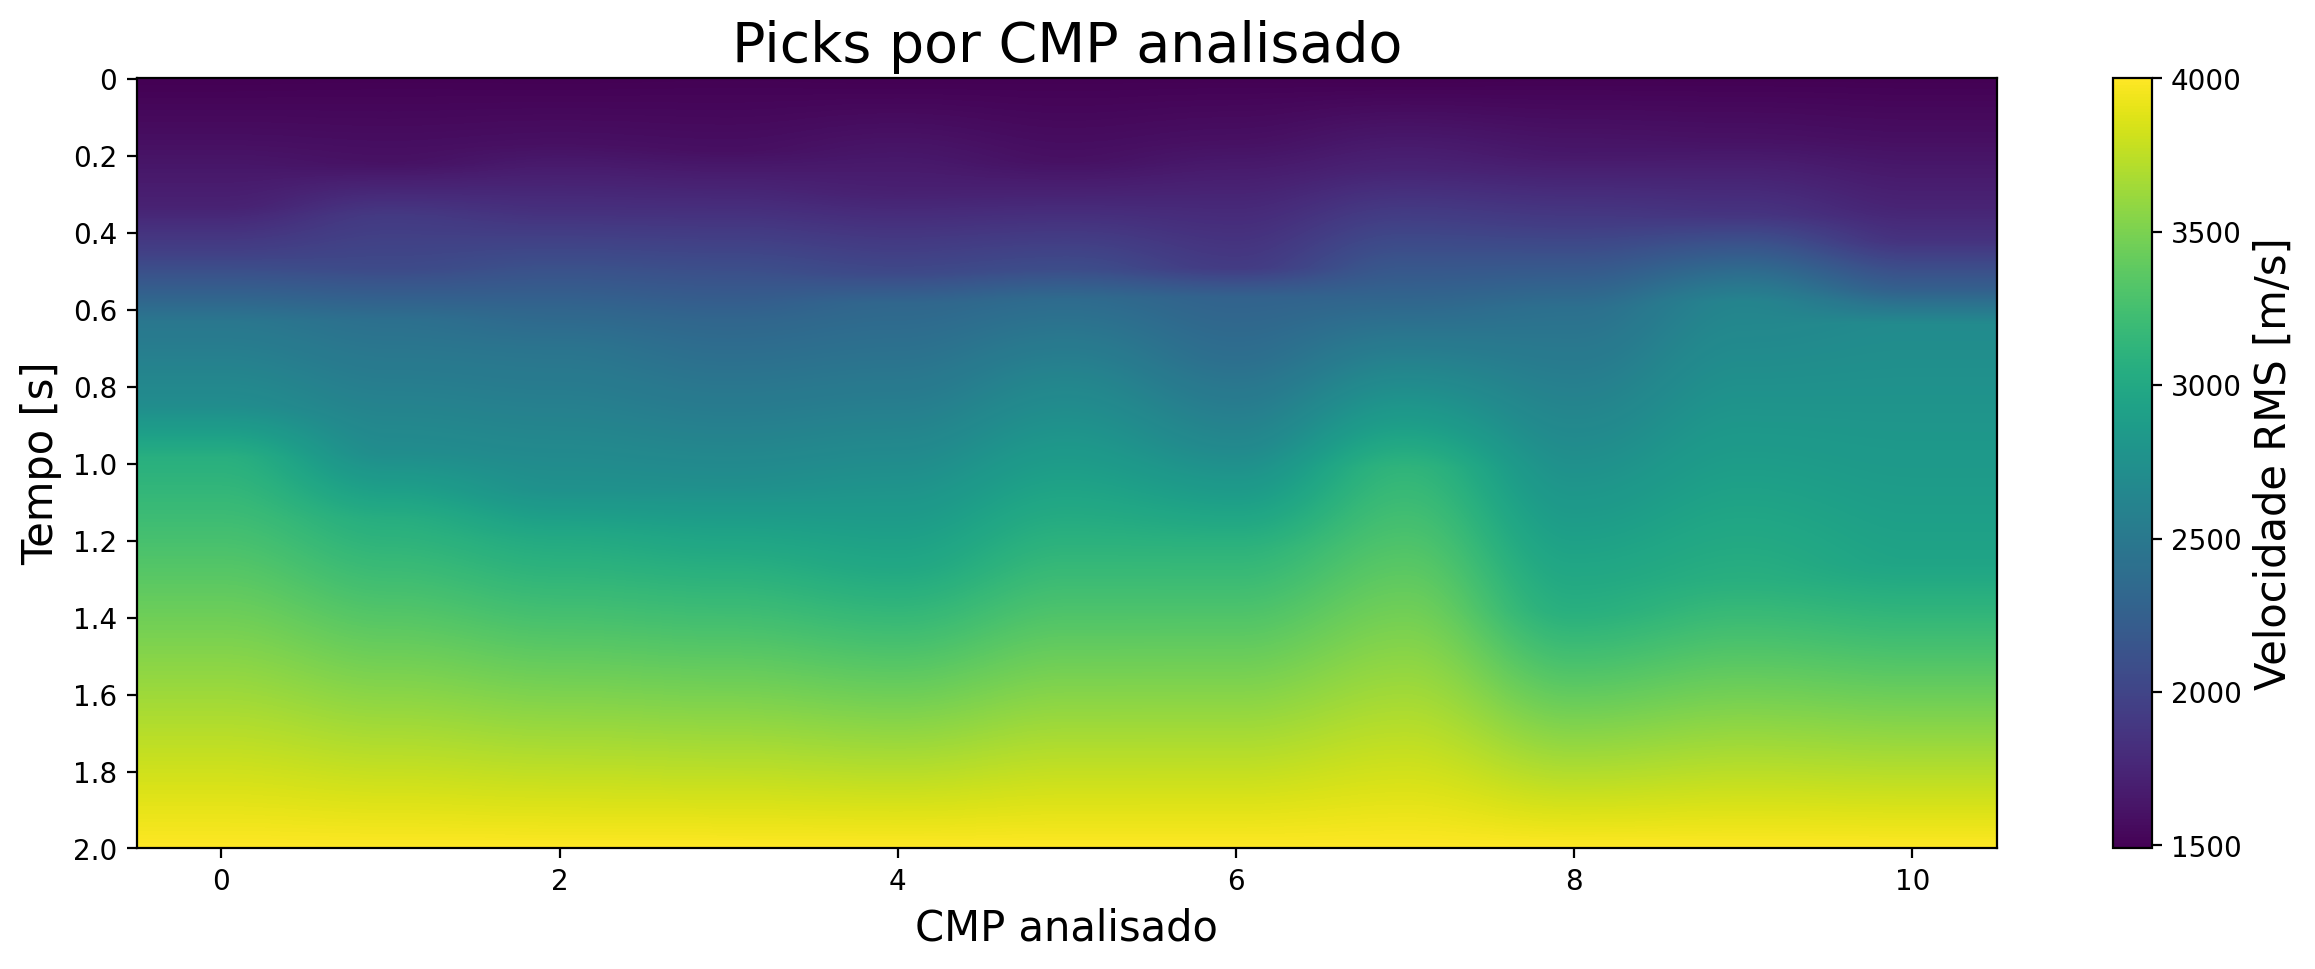
\includegraphics[width=16cm,height=7.5cm]{../imagens/picksInterpVertical.png}
		\caption{\textit{Arrays} de velocidade RMS dos sismogramas CMP analisados interpolados linearmente utilizando o interpolador implementado pelo autor.}
		\label{picksVertInterp}
	\end{figure}

	As posições dos sismogramas CMP são bem estabelecidas na geometria genérica. Então, após a interpolação na vertical das velocidades RMS, ou seja, no domínio do tempo, os \textit{arrays} de dado foram postos numa matriz com número de colunas na quantidade das posições de pontos médios comum de varredura completa. Seguindo o raciocínio, existiriam colunas com velocidades RMS com todos os tempos preenchidos e outras colunas completamente vazias. Neste sentido, uma interpolação linear regular foi implementada para preencher as colunas sem dados de velocidade RMS. 
	
	A figura \ref{modeloRMSCMPsCompletos}, mostra o resultado da interpolação completa do modelo de velocidade RMS com domínios de tempo e CMPs de varredura completa. O objetivo da estimativa de velocidades seria obter o campo de velocidade intervalar do meio, porém, antes da conversão, foi feito uma suavização no modelo de vagarosidade RMS para evitar mudanças abruptas de velocidade intervalar durante a conversão.  

    \begin{figure}[htp!]
		\centering
		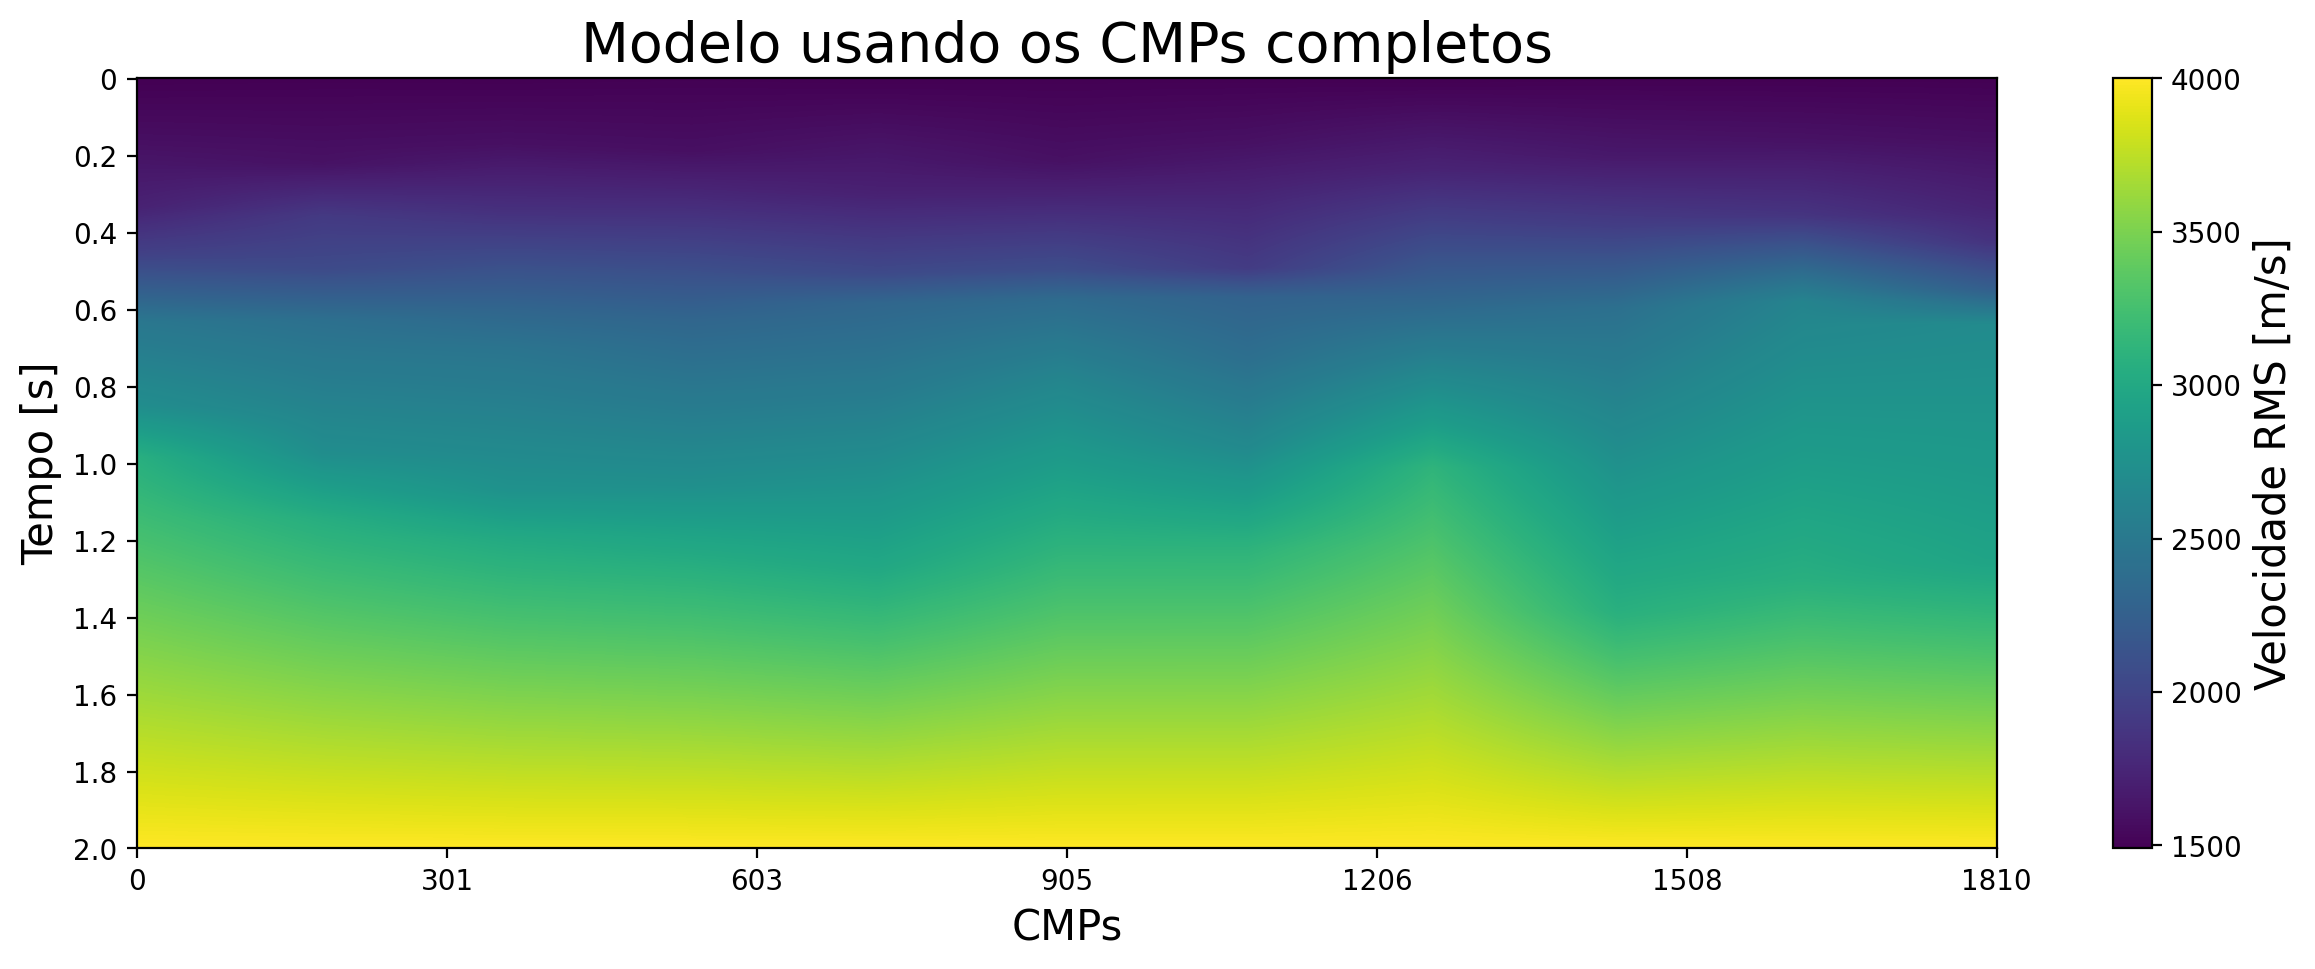
\includegraphics[width=16cm,height=7.5cm]{../imagens/modeloCompleto.png}
		\caption{Modelo de velocidade RMS interpolado a partir dos pontos de velocidade extraídos do arquivo gerado através do método da análise de velocidade.}
		\label{modeloRMSCMPsCompletos}
	\end{figure}

	A figura \ref{modeloSuavizadoRMS}, mostra o modelo suavizado. O processo de suavização ocorreu na vagarosidade, ou seja, a grandeza suavizada foi o inverso da velocidade. O algoritmo suavizador pertence ao pacote \textit{Seismic Unix} chamado \textit{smooth2}, que utiliza a técnica da suavização por mínimos quadrados (\textit{least square smoothing}). Foi utilizado o parâmetro 10 em ambas dimensões.   

	Após a suavização do modelo de vagarosidade RMS, a conversão para velocidade intervalar foi realizada. A figura \ref{modeloSuavizadoINT}, mostra o resultado da conversão de velocidades utilizando a equação \ref{dix}, sendo observado, na parte próxima de 2 segundos, artefatos   gerados pelo processo de interpolação, pois a velocidade na região não foi estimada.

	\newpage
    \begin{figure}[htp!]
		\centering
		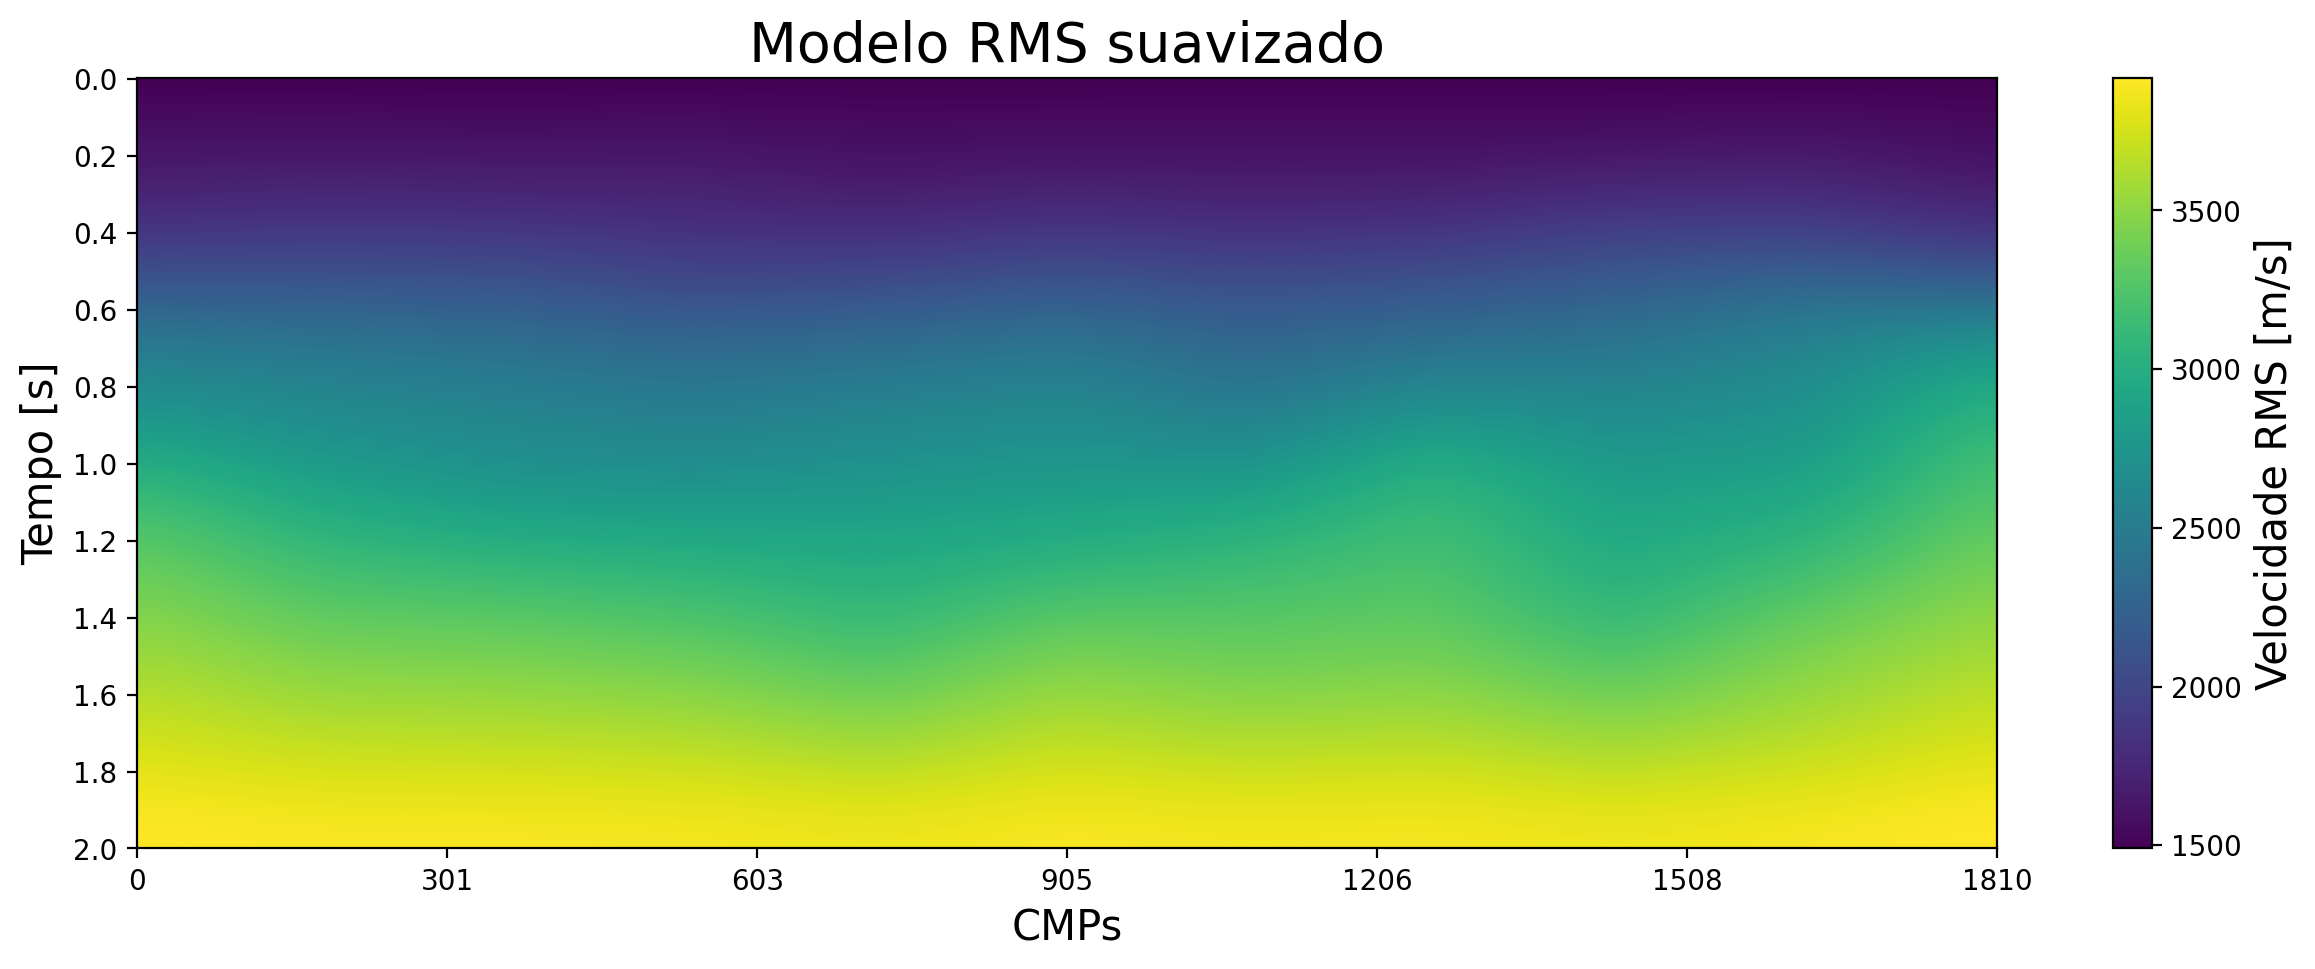
\includegraphics[width=16cm,height=7.5cm]{../imagens/modeloSuavizadoRMS.png}
		\caption{Modelo de velocidade RMS suavizado pelo programa \textit{smooth2} do pacote \textit{Seismic Unix}, utilizando os parâmetros de suavização 10 para ambas dimensões.}
		\label{modeloSuavizadoRMS}
	\end{figure}

	O modelo de velocidades intervalares foi construído até 1,4 segundos para otimizar o processo de modelagem sísmica, obtendo um modelo truncado na amostra vertical de 350 e contendo 1810 amostras na horizontal (Figura \ref{modeloSuavizadoINTUTIL}).  	

    \begin{figure}[htp!]
		\centering
		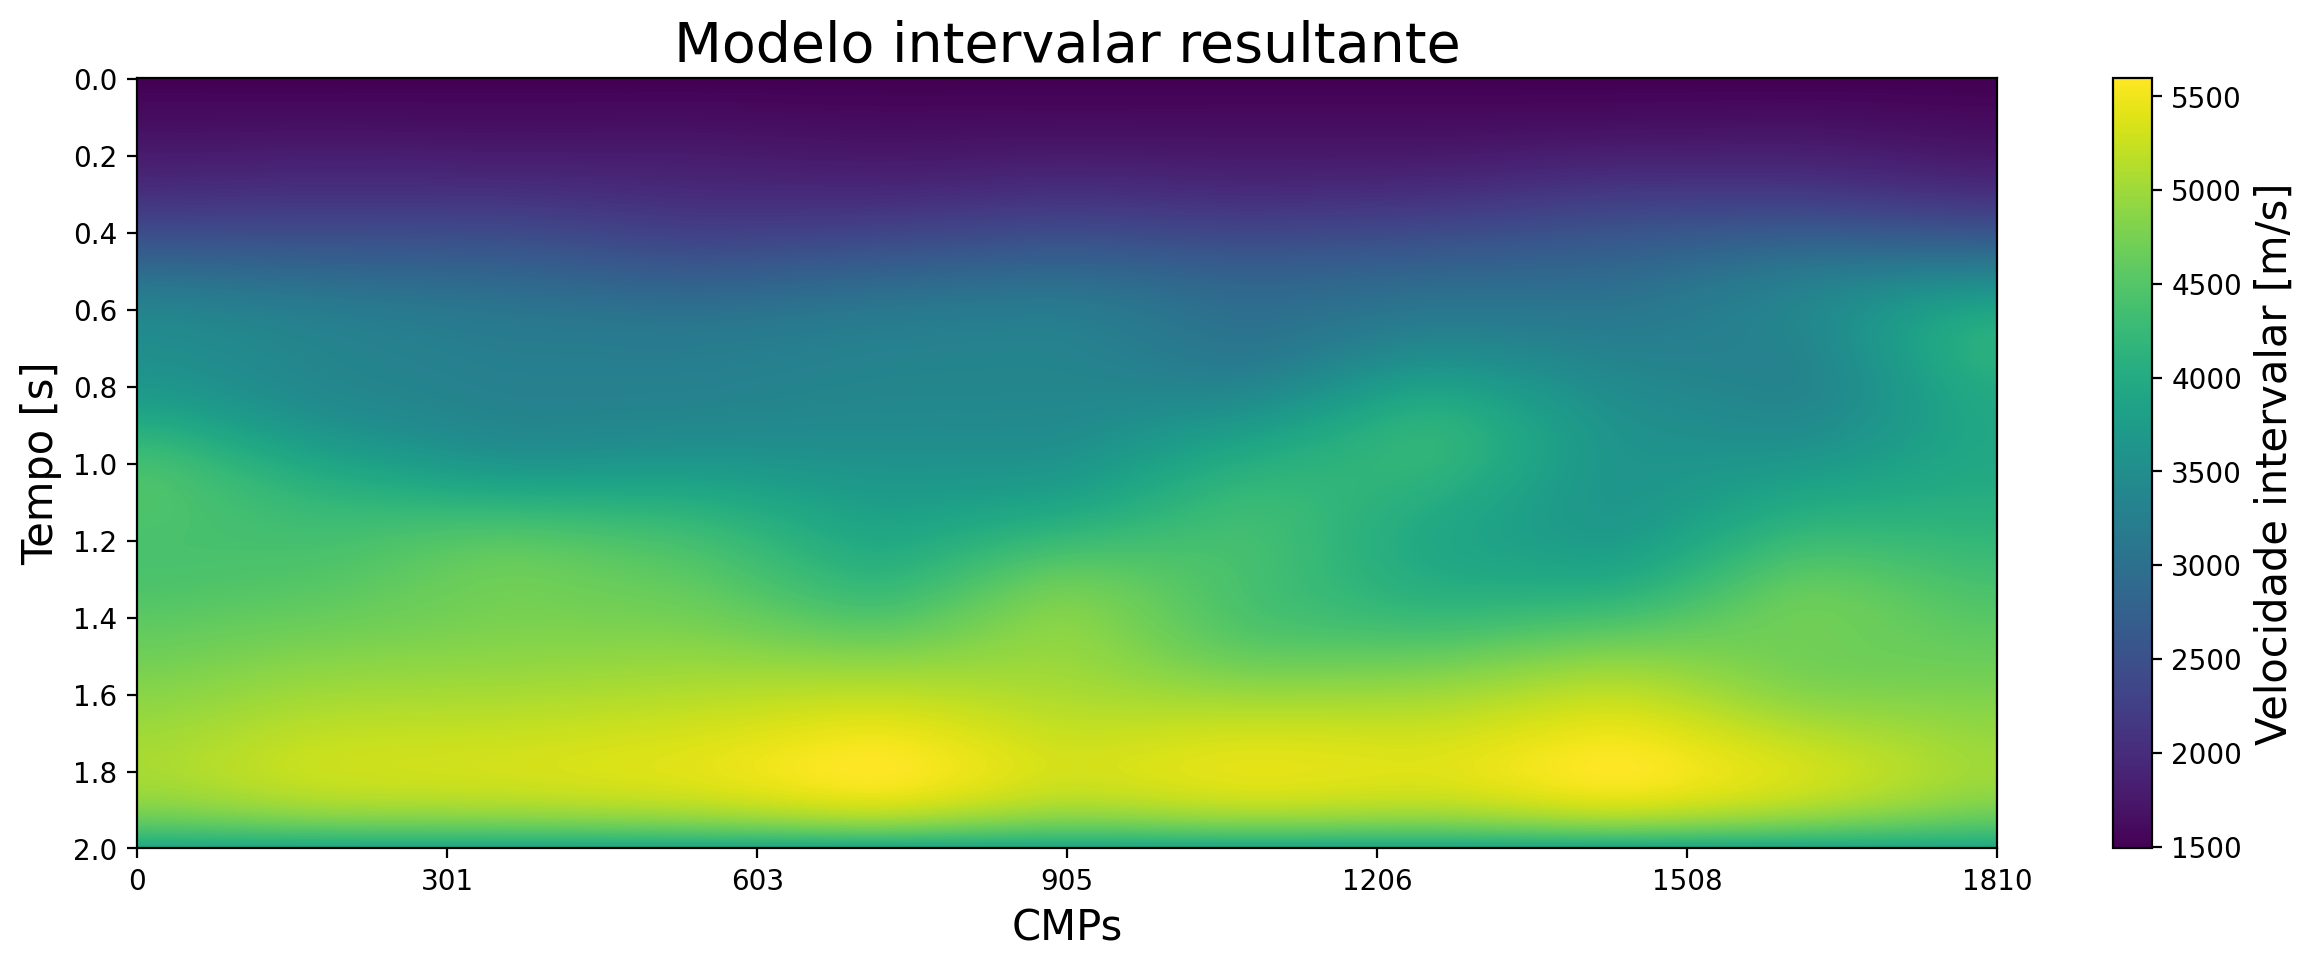
\includegraphics[width=16cm,height=7.5cm]{../imagens/modeloSuavizadoINT.png}
		\caption{Modelo de velocidades gerado a partir da conversão de velocidade RMS para intervalar. Pela aplicação forçada de uma velocidade RMS nos tempos próximos a 2 segundos, o modelo recebeu valores inconsistentes na região após a conversão.}
		\label{modeloSuavizadoINT}
	\end{figure}

    \begin{figure}[htp!]
		\centering
		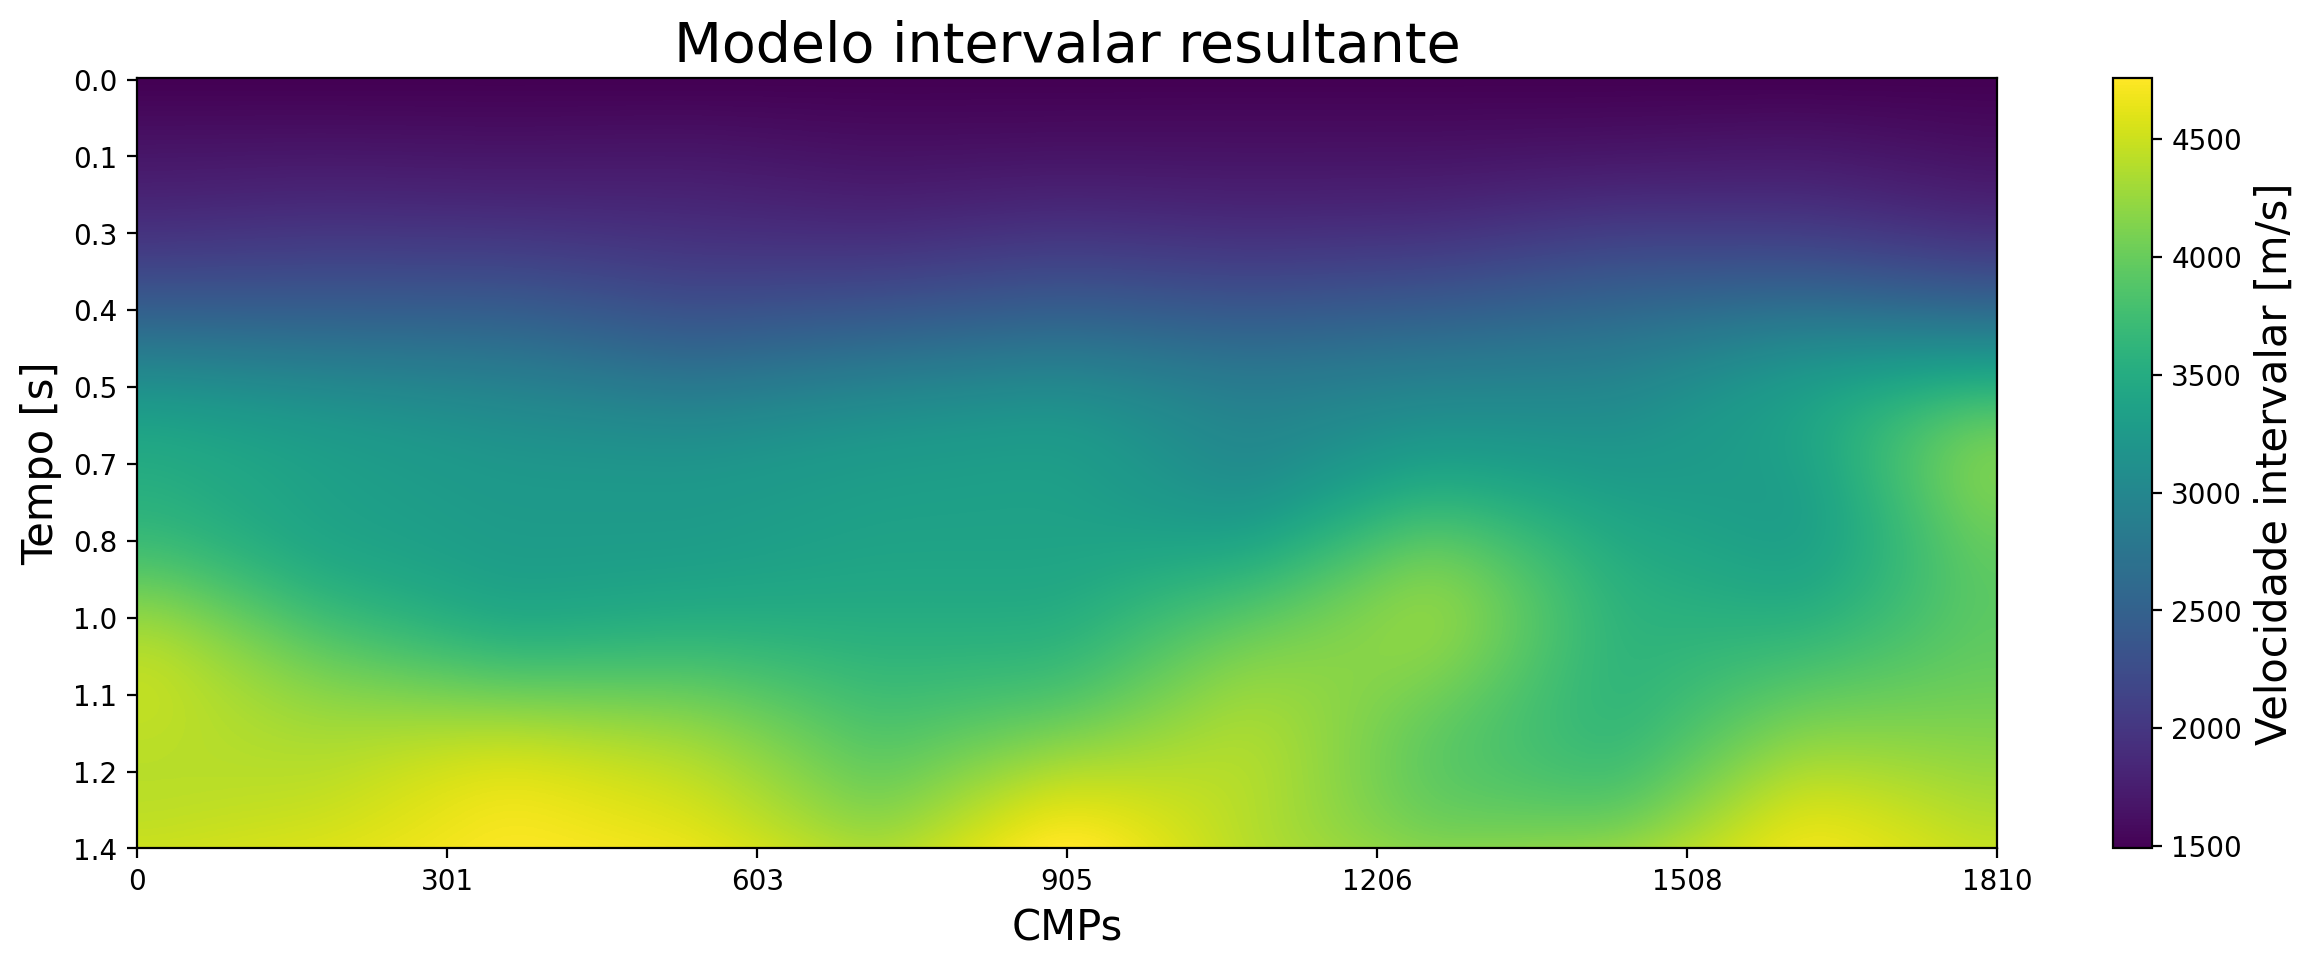
\includegraphics[width=16cm,height=7.5cm]{../imagens/modeloSuavizadoINTUTIL.png}
		\caption{Redução do modelo de velocidades intervalares para otimizar o número de amostras na vertical.}
		\label{modeloSuavizadoINTUTIL}
	\end{figure}

	Para simular a aquisição sísmica, o modelo de velocidades deve comportar toda a geometria de receptores e fontes presentes na aquisição. A estimativa do modelo foi feita apenas para os pontos médios comuns de varredura completa. Então, para adaptar o modelo em uma simulação sísmica, foi realizada a extrapolação das velocidades nas laterais. O primeiro passo foi encaixar o modelo numa matriz que contempla toda a aquisição (figura \ref{modeloReduzidoINT}), com dimensões horizontais de 2772 amostras e 12,5 metros como parâmetro de discretização, originando 34650 metros de aquisição sísmica.
	
    \begin{figure}[htp!]
		\centering
		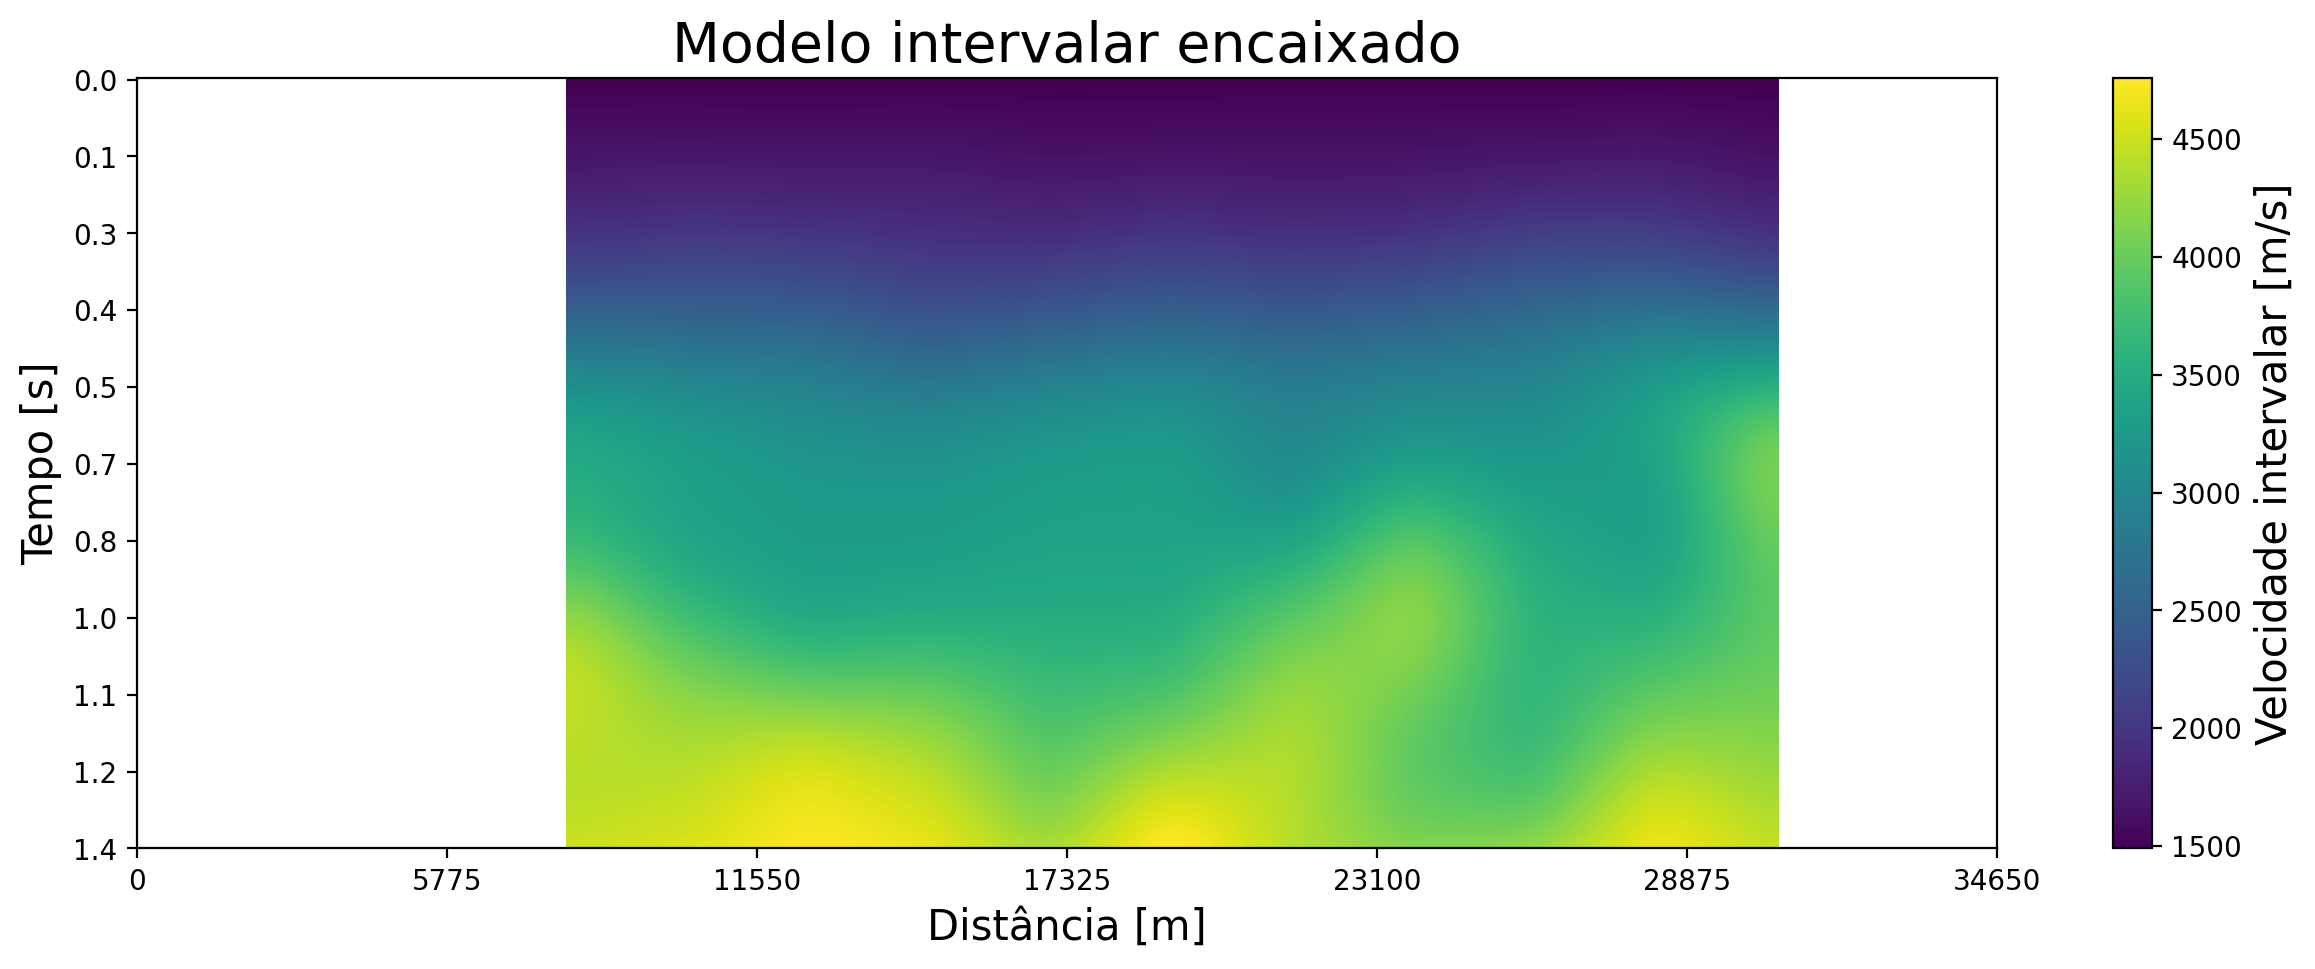
\includegraphics[width=16cm,height=7.5cm]{../imagens/modeloReduzidoINT.png}
		\caption{Modelo de velocidades intervalares encaixado para posteriormente ser realizada a extrapolação das laterais.}
		\label{modeloReduzidoINT}
	\end{figure}

    \begin{figure}[htp!]
		\centering
		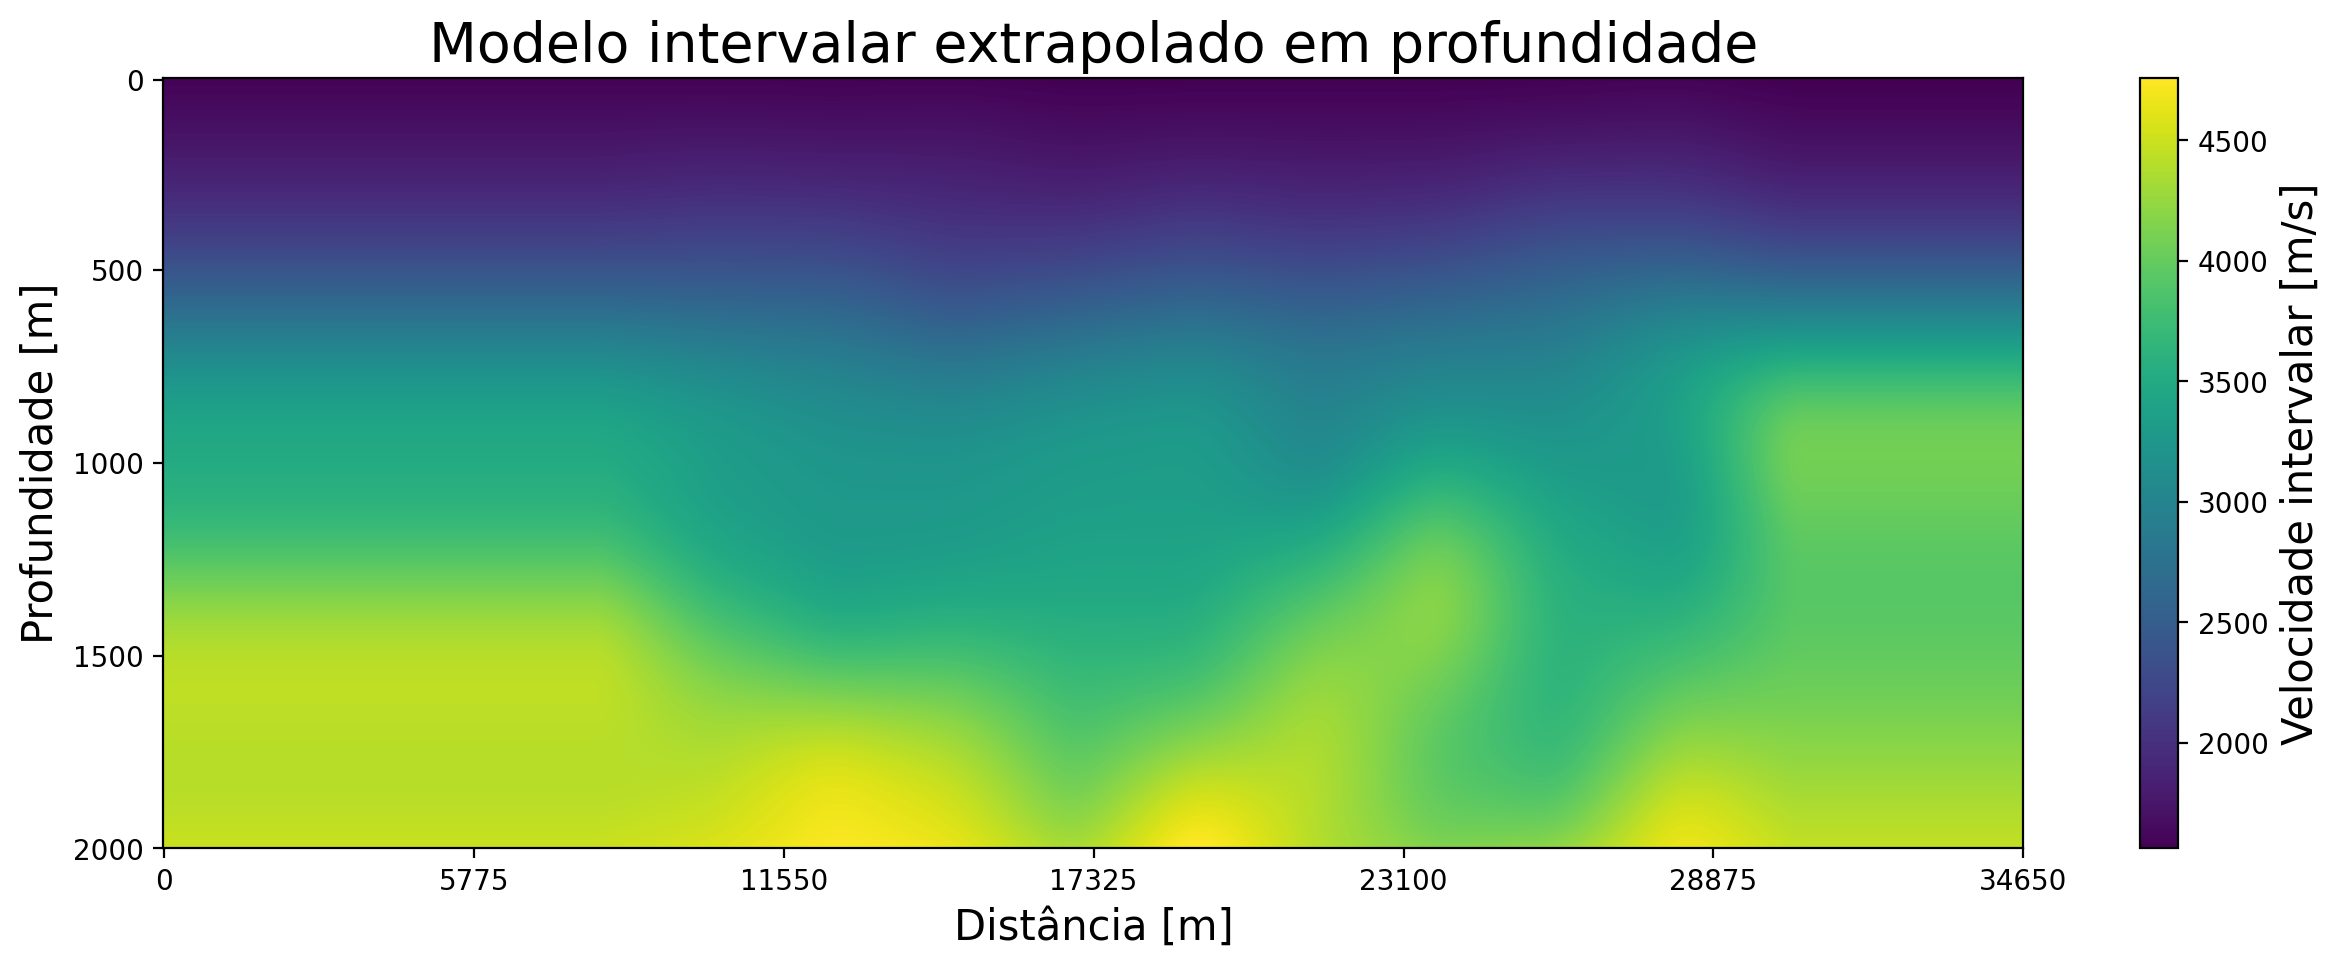
\includegraphics[width=16cm,height=7.5cm]{../imagens/modeloExtrapoladoINT.png}
		\caption{Modelo de velocidades intervalares estimado em profundidade.}
		\label{modeloExtrapoladoINT}
	\end{figure}
	
	Após o encaixe do modelo, as laterais foram preenchidas com a informação da primeira e última coluna do modelo formadas pelos CMPs completos. Como mostrado na figura \ref{modeloExtrapoladoINT}, a conversão tempo-profundidade foi executada baseada no parâmetro de discretização temporal do dado real, multiplicando cada ponto de velocidade por este parâmetro e dividindo pela metade, por consequência do dado ser de tempo duplo de propagação. Esse procedimento foi feito por colunas da matriz modelo, cada coluna com sua profundidade. Então uma média das profundidades por coluna foi realizada. Ao definir uma profundidade, o parâmetro de discretização na vertical foi calculado, dividindo a profundidade pelo número de amostras na vertical. 
	
	O fundo do mar foi ajustado na profundidade ideal, aproximando a velocidade da camada de água $v$ como 1500 m/s. Calculando então a distância em metros até o fundo do mar $d$ a partir do tempo duplo $t$ até o horizonte e pela metade do \textit{offset} mínimo $O_m$ do dado, tem-se a formulação para velocidade $v$ homogênea no formato
%	
	\begin{equation}
		d = \sqrt{\left(\dfrac{vt}{2}\right)^2 + \left(\dfrac{O_m}{2}\right)^2}.
	\end{equation}	
	
	 A quantidade de amostras na parte superior do modelo foi ajustada para encaixar o horizonte do fundo marinho na posição correta em profundidade e os demais horizontes foram encaixados de acordo com suas respectivas amostras.
	
\section{Empilhamento do dado real}

	O dado empilhado será o objeto de comparação deste trabalho, onde o dado real será comparado com o dado sintético a partir do empilhamento e migração em tempo de ambos. Realizando o processo de empilhamento no dado real obtém-se a seção exibida na figura \ref{empilhamentoReal}, migrada em tempo. O processo de migração em tempo foi empregado a partir da técnica de \citeonline{stolt1978migration} pós-empilhamento, implementada no pacote \textit{Seismic Unix}. A migração em tempo pós-empilhamento visa a colapsar as hipérboles de difração em seus ápices, para que a seção tenha melhorias nos aspectos de continuidade lateral. 
	
	\newpage 
	Utilizando o algoritmo do \textit{Seismic Unix}, as velocidades obtidas no processo de análise de velocidades foram parâmetros de entrada, juntamente com a quantidade de CMPs de varredura completa e suas distâncias em metro entre si. 

	\begin{figure}[htp!]
		\centering
		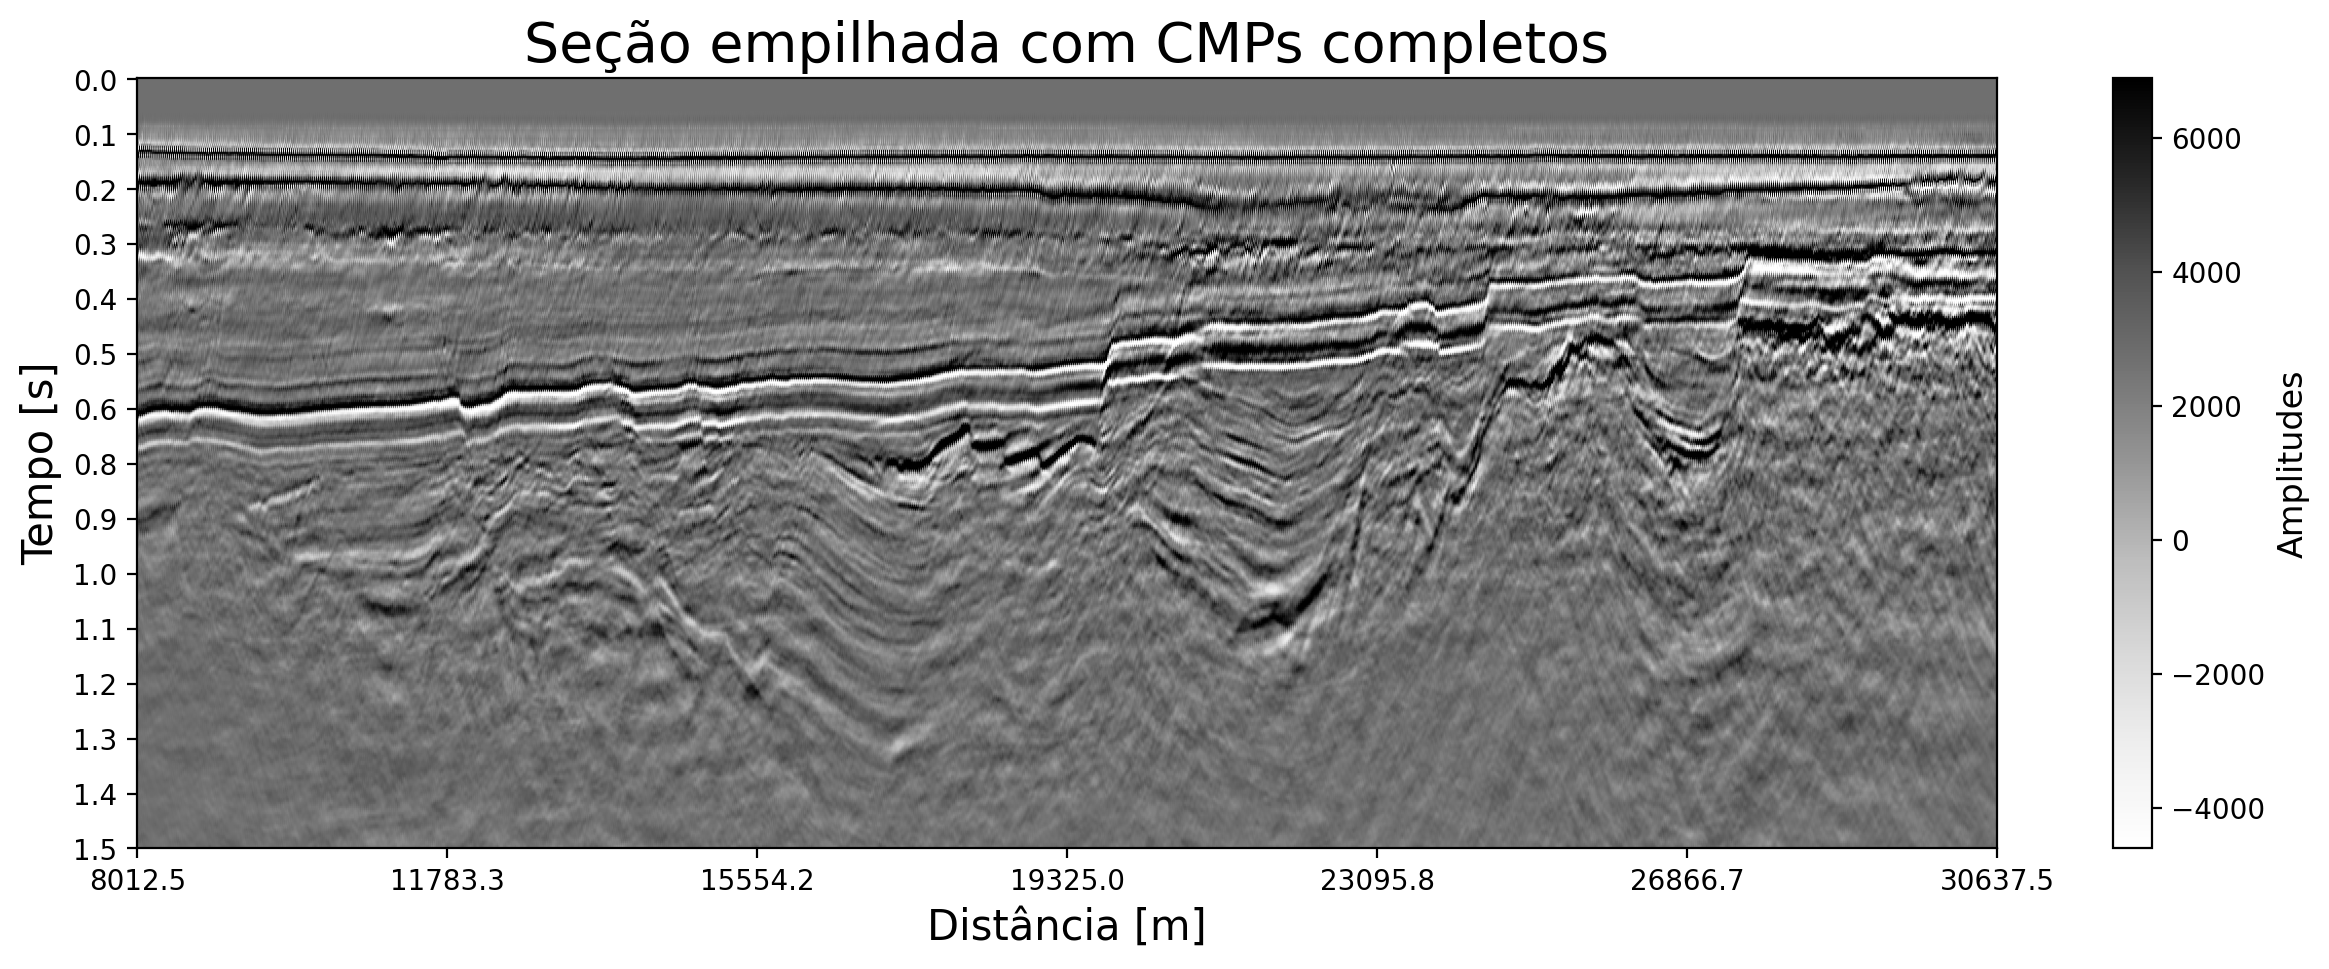
\includegraphics[width=16cm,height=7cm]{../imagens/sectionReduced.png}
		\caption{Seção empilhada e migrada em tempo do dado real da margem sudoeste da Inglaterra. A partir de 1,5 segundos as informações são escassas. As amplitudes do dado se referem às que vieram do pré-processamento desconhecido. Redução até o tempo 1,5 segundos para efeito de comparação entre seções.}
		\label{empilhamentoReal}
	\end{figure}	

	Sabendo que após 1,5 segundos de tempo duplo, a seção empilhada possui informações de reflexão muito ruidosas, o tempo escolhido para comparar o dado real com sintético foi de 1,5 segundos. Redução feita para otimizar o tempo de simulação na modelagem sísmica. A figura \ref{empilhamentoReal} mostra o dado reduzido e preparado para futuras comparações e análises. 

\section{Construção dos modelos de propriedades elásticas}
	
	A validação do modelo foi feita a partir de uma modelagem sísmica, replicando com máxima similaridade as propriedades de aquisição, para meios elásticos isotrópicos. Então, somente o modelo de velocidade da onda compressional não é o suficiente para representar uma propagação de ondas em meio elástico. O procedimento desenvolvido neste trabalho foi a coleta de horizontes da seção empilhada do dado real ao ponto de construir um modelo abrupto para ser a base das propriedades elásticas restantes, a velocidade da onda cisalhante e a densidade.
	
	A coleta de horizontes ocorreu a partir da importação da seção empilhada em um programa de ilustrações - \textit{Inkscape}, dimensionando a quantidade de \textit{pixels} da imagem igual a quantidade de amostras da sísmica. 
	
	\newpage
	Após a leitura da imagem no programa, os horizontes foram interpretados e salvos em forma de imagem (Figura \ref{desenhoHorizontes}) com cores no formato RGB (\textit{Red}, \textit{Green}, \textit{Blue}). A escala de cores RGB possui um esquema específico de numeração, variando de 0 a 255 para cada cor. 
	
    \begin{figure}[htp!]
		\centering
		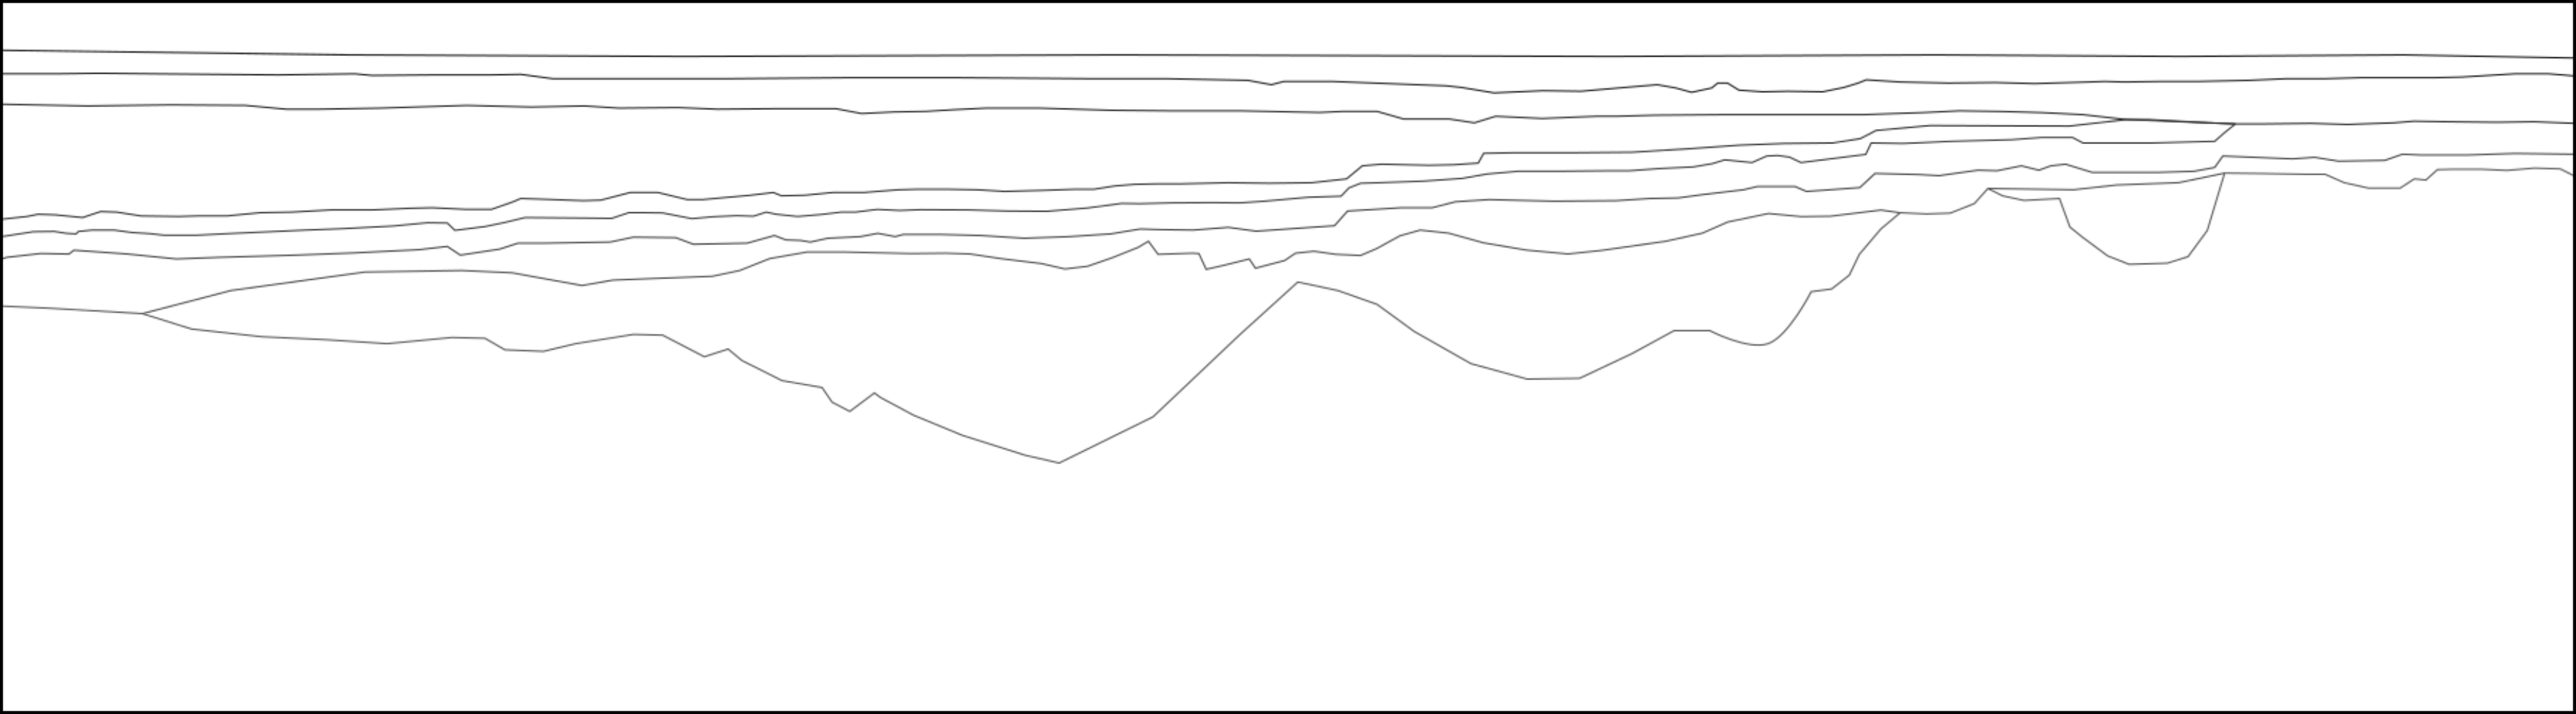
\includegraphics[width=16cm,height=4cm]{../imagens/horizontes.png}
		\caption{Horizontes desenhados a partir do \textit{software} de ilustrações \textit{Inkscape}. Imagem importada posteriormente em um programa python que coletou, a partir de cada \textit{pixel}, as posições em amostra dos horizontes interpretados.}
		\label{desenhoHorizontes}
	\end{figure}
	
	Sabendo dessa informação, a imagem dos horizontes interpretados (Figura \ref{desenhoHorizontes}) foi importada em um programa na linguagem python desenvolvido pelo autor. Cada \textit{pixel} da imagem recebeu um número dentro de uma matriz e as posições dos horizontes foram recolhidas a partir desses números, na mesma dimensão da seção sísmica empilhada (Como mostrado na figura \ref{sismicaHorizontes}).     
	
	\begin{figure}[htp!]
		\centering
		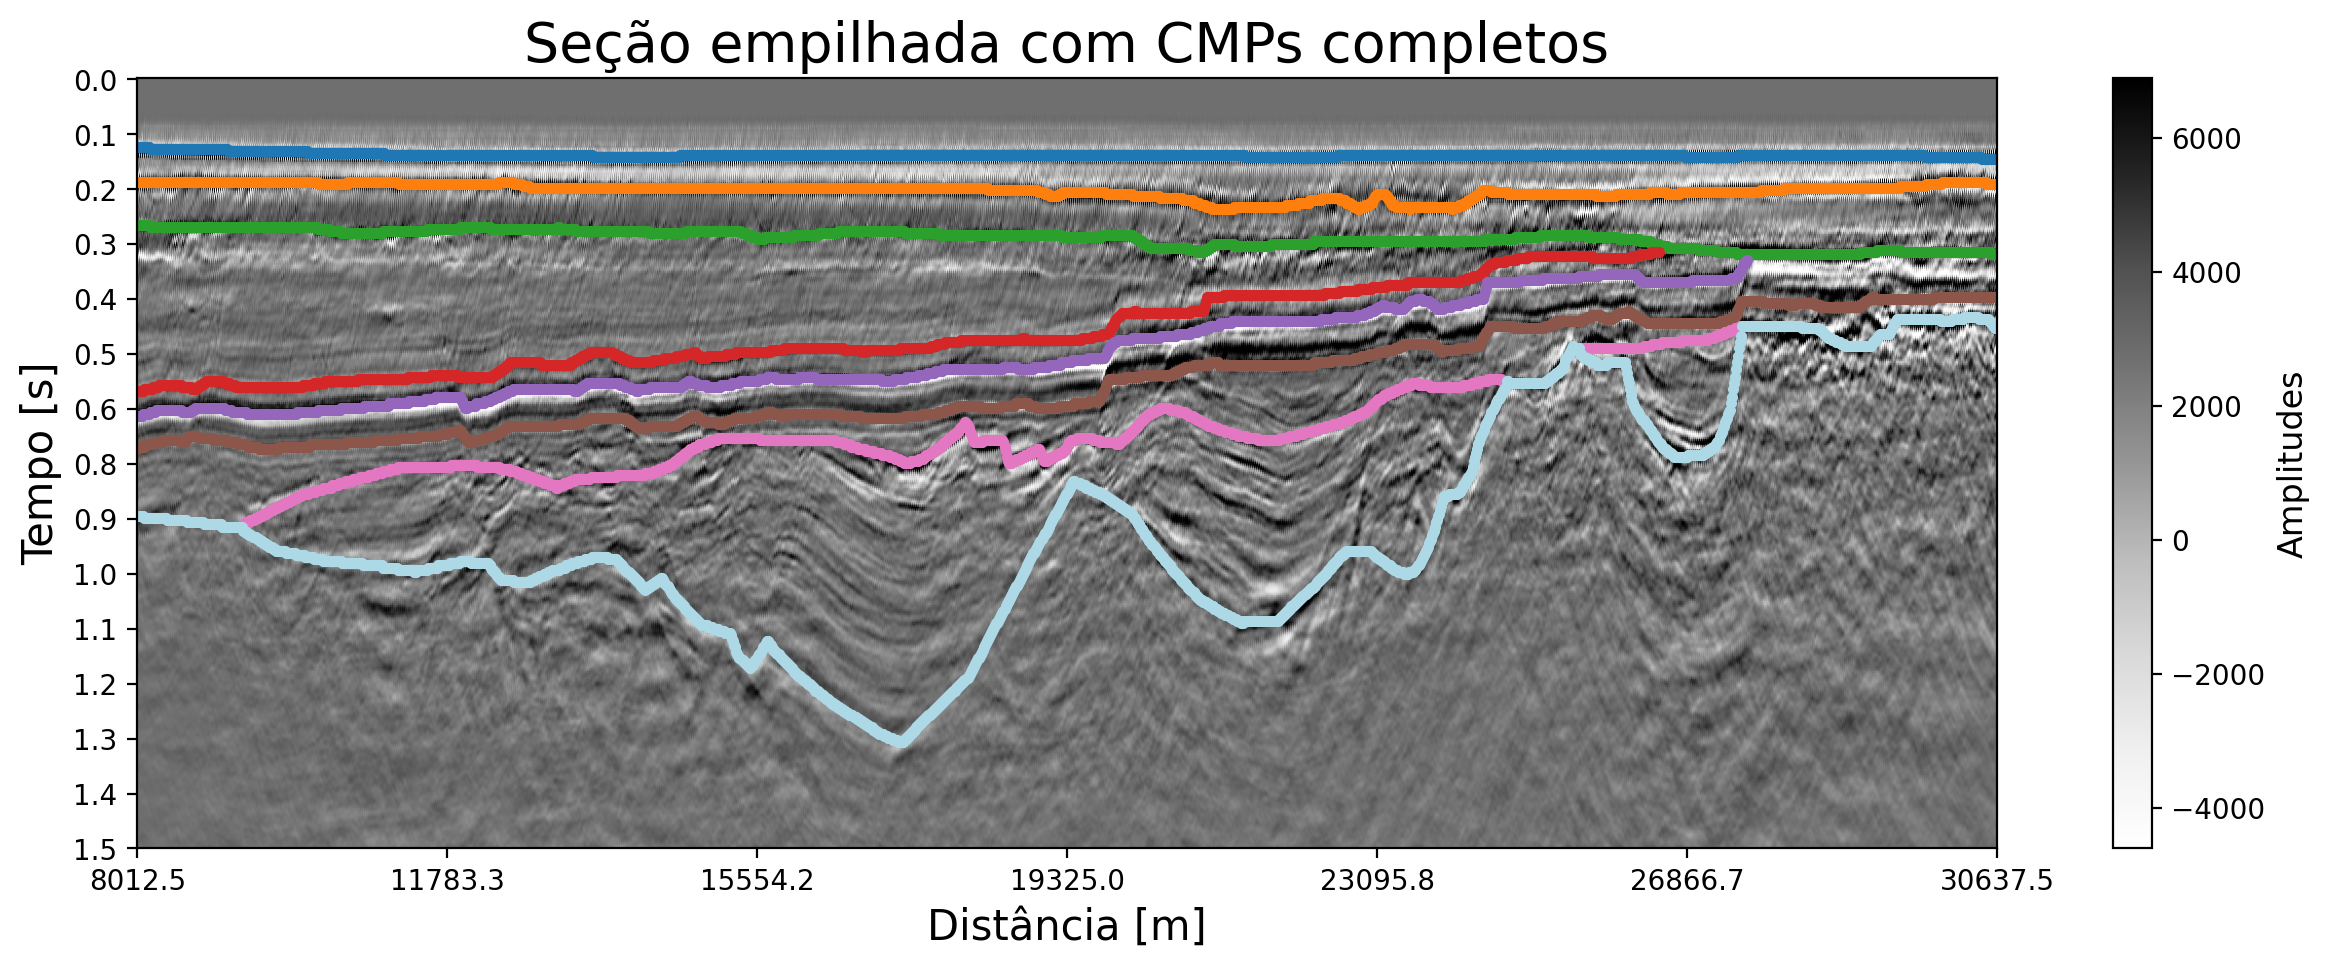
\includegraphics[width=16cm,height=7cm]{../imagens/sectionHrz.png}
		\caption{Seção empilhada e migrada do dado real com horizontes projetados.}
		\label{sismicaHorizontes}
	\end{figure}

	A figura \ref{modeloHorizontes}, mostra a configuração dos horizontes convertidos para profundidade projetados no modelo estimado. A partir das posições em amostra dos horizontes, foi construído um modelo de velocidade da onda compressional abrupto (Figura \ref{modeloAbrupto}) baseado nas velocidades médias, constante por horizonte, do modelo de velocidades intervalares estimado anteriormente.  
	
	As propriedades de velocidade cisalhante e densidade são estimadas a partir do modelo abrupto construído e ilustrado na figura \ref{modeloAbrupto}.  

	\begin{figure}[htp!]
		\centering
		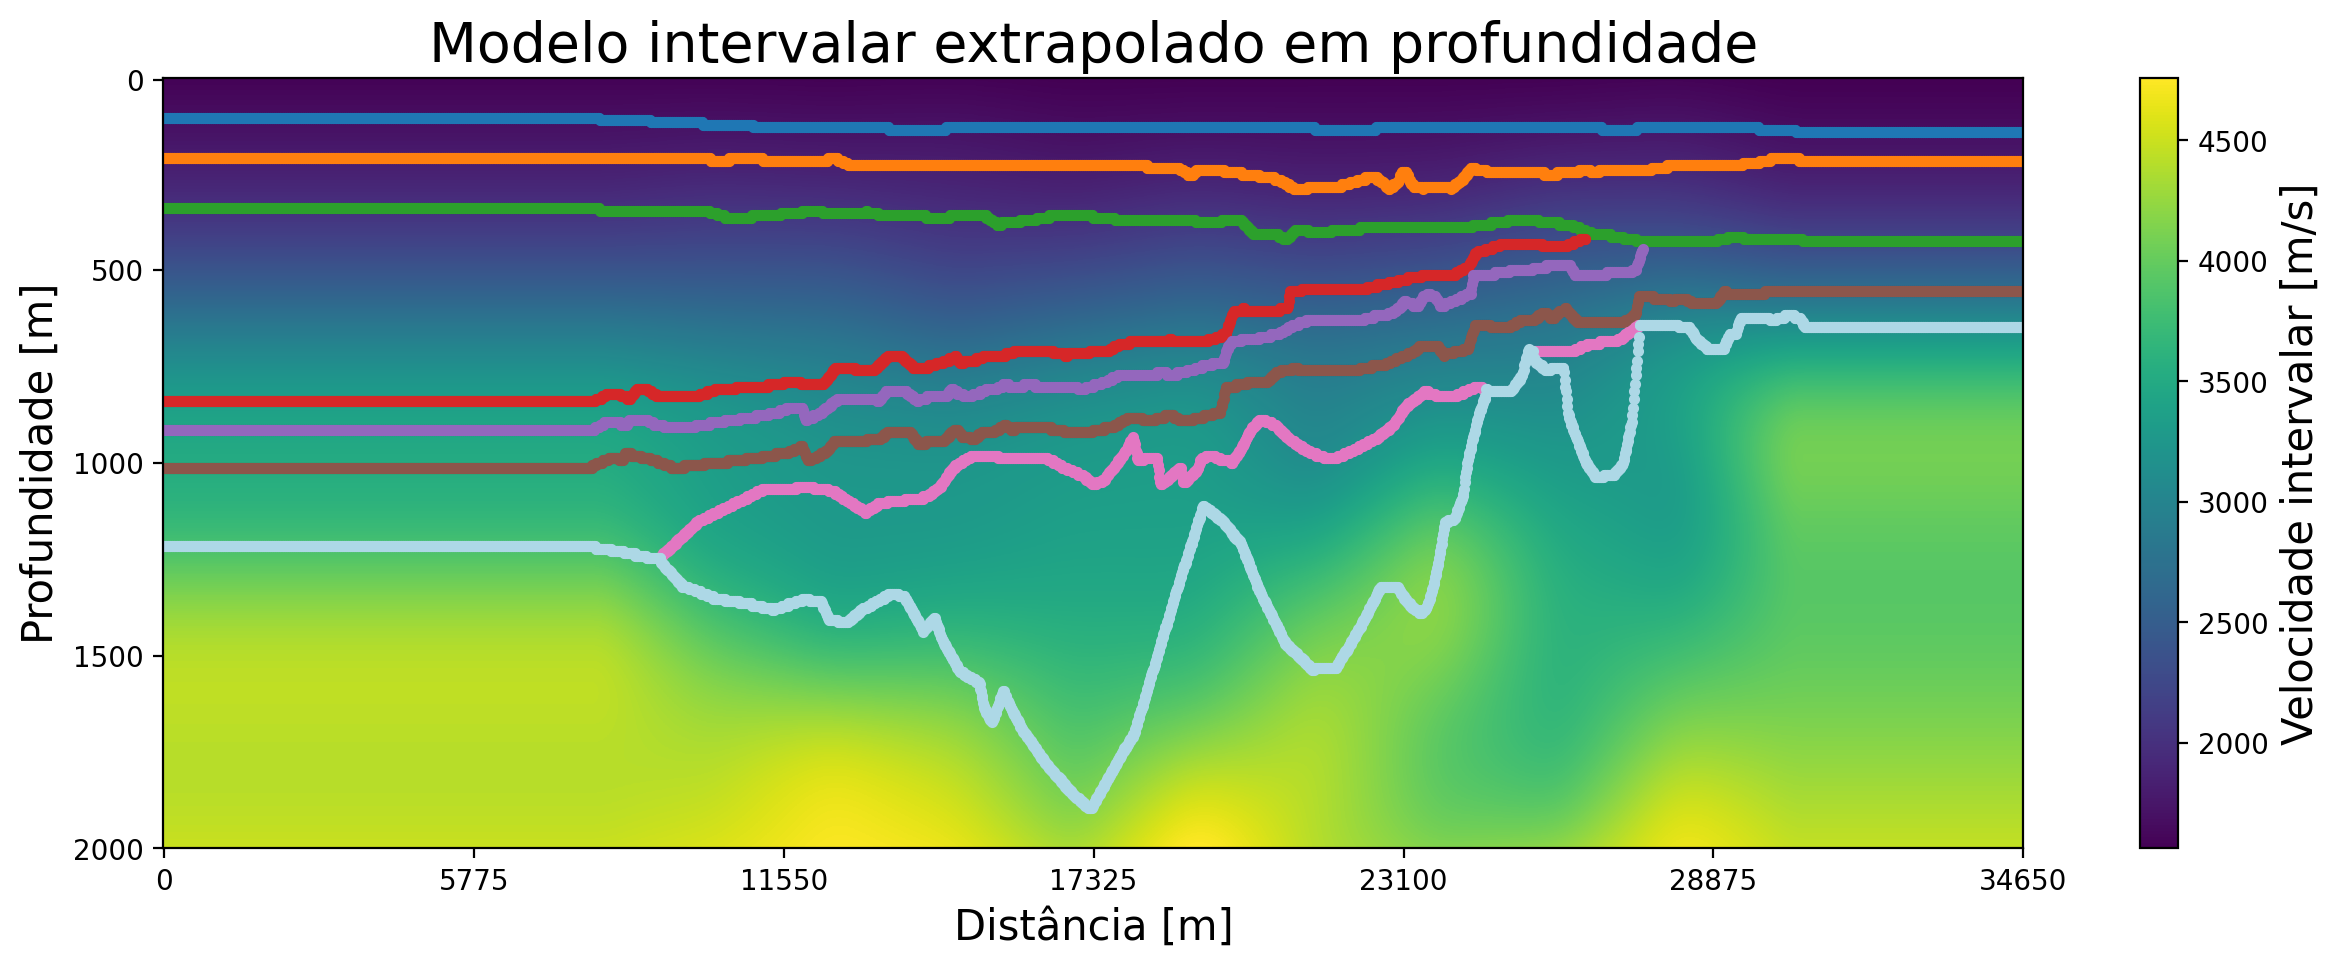
\includegraphics[width=16cm,height=7cm]{../imagens/modeloExtrapoladoINTHRZ.png}
		\caption{Modelo de velocidades da onda compressional com horizontes projetados.}
		\label{modeloHorizontes}
	\end{figure}

	\begin{figure}[htp!]
		\centering
		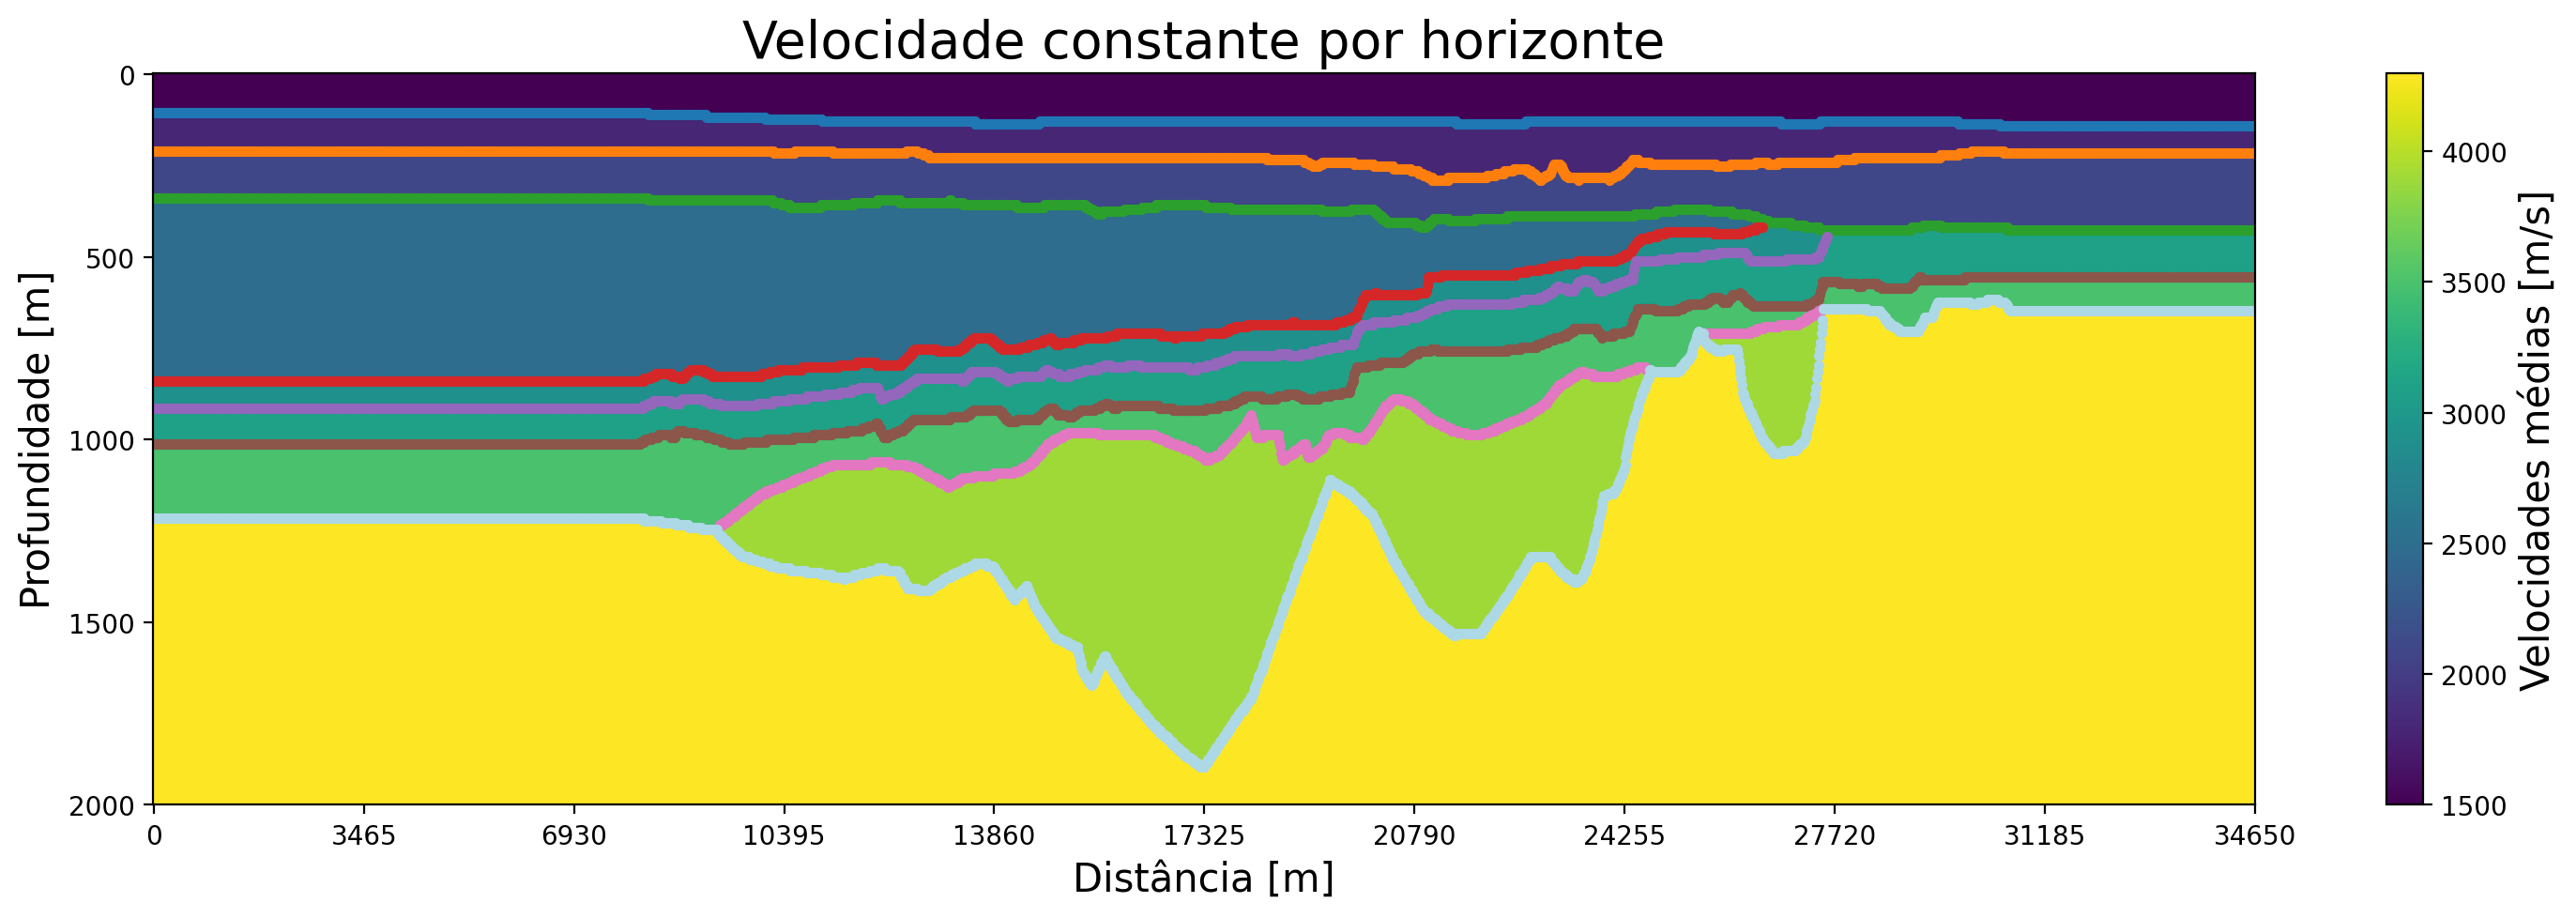
\includegraphics[width=16cm,height=7cm]{../imagens/modeloAbrupto.png}
		\caption{Modelo abrupto de velocidades da onda compressional baseado nas velocidades médias do modelo estimado. O modelo abrupto será utilizado para gerar a estimativa das velocidades cisalhantes e das densidades.}
		\label{modeloAbrupto}
	\end{figure}

\section{Simulação da aquisição sísmica}
	
	A validação da estimativa será empregada a partir de uma modelagem sísmica para meios elásticos isotrópicos obedecendo as características da aquisição.	Os modelos abrupto e suave mostrados anteriormente nas figuras \ref{modeloHorizontes} e \ref{modeloAbrupto} respetivamente, tem discretizações espaciais diferentes. Na dimensão horizontal, eixo da distância, o modelo tem 34650 metros com 12,5 metros de discretização totalizando 2772 amostras. 
	
	Na dimensão vertical, eixo da profundidade, o modelo tem 2000 metros com 323 amostras, efetuando a divisão do tamanho em metros pela quantidade de amostras obtém-se o parâmetro de discretização de 6,192 metros.

	Para a realização da modelagem sísmica, o modelo de propriedades foi alterado na dimensão horizontal, resultando uma discretização espacial mais próxima do eixo da profundidade. O procedimento realizado foi aumentar o modelo de propriedades, na forma que ele dobrasse de tamanho, para obter um parâmetro de discretização pela metade do original. Assim o modelo passou de 2772 para 5544 amostras na horizontal com discretização de 6,25 metros. Os modelos são mostrados na figura \ref{modeloInput}. 
	
	A aplicação das bordas foi realizada com 50 pontos de extrapolação do modelo para todas as direções, aumentando as dimensões do modelo para 5644 x 423 amostras. O parâmetro de atenuação da borda de \citeonline{cerjan1985nonreflecting} foi 0,0045 para este trabalho. Uma condição especial nas quinas foi desenvolvida para atenuação em duas dimensões com o objetivo de atenuar melhor ângulos de incidência diferentes de 90 graus. Um programa externo ao \textit{script} de modelagem sísmica gera a matriz de atenuação, onde na região do modelo, a matriz possui valores iguais a 1 e nas bordas, a equação de atenuação é utilizada.

	\begin{figure}[htp!]
		\centering
		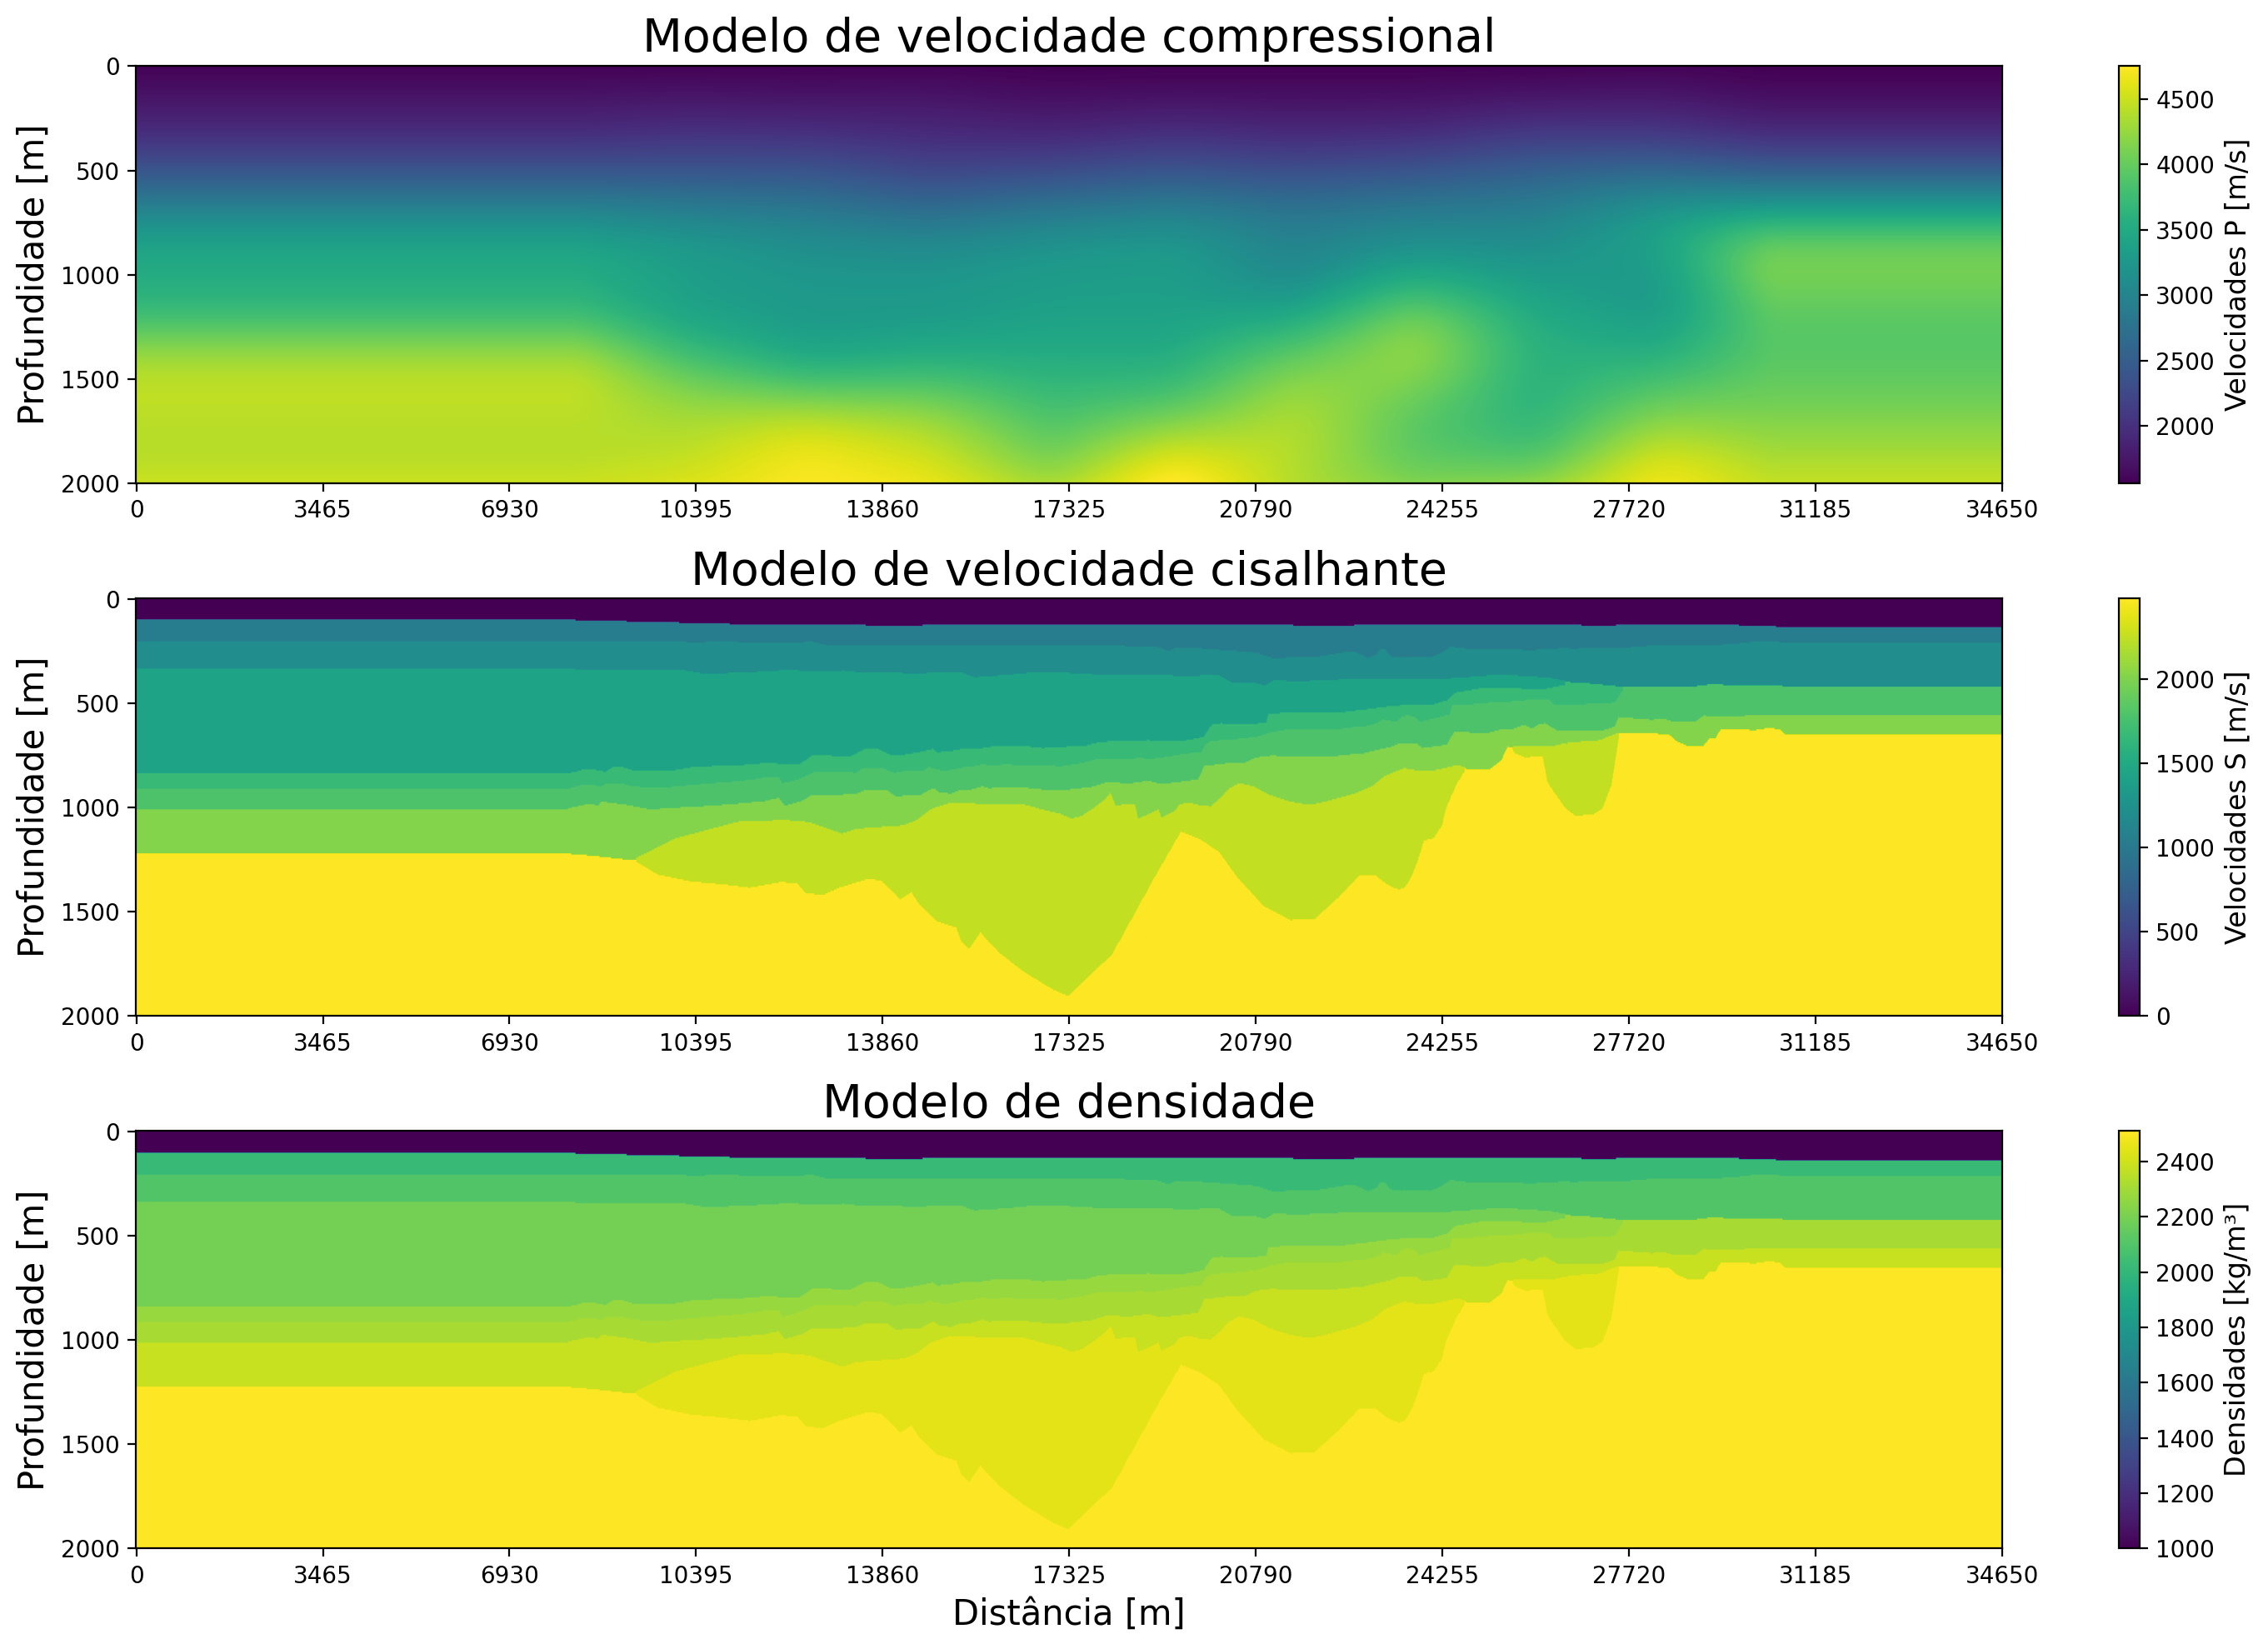
\includegraphics[width=16cm,height=11cm]{../imagens/ModelosInput.png}
		\caption{Modelos de velocidade da onda P, velocidade da onda S e densidade estimados para o processo de modelagem sísmica em meios elásticos isotrópicos sem a aplicação das bordas de atenuação.}
		\label{modeloInput}
	\end{figure}

	\newpage
	A assinatura da fonte foi estimada a partir da seção de \textit{offset} comum, onde foi feito uma janela de tempo em torno da primeira reflexão (reflexão do fundo marinho, figura \ref{westim}). As amplitudes dos traços foram somadas e divididas pela quantidade de traços.

	\begin{figure}[htp!]
		\centering
		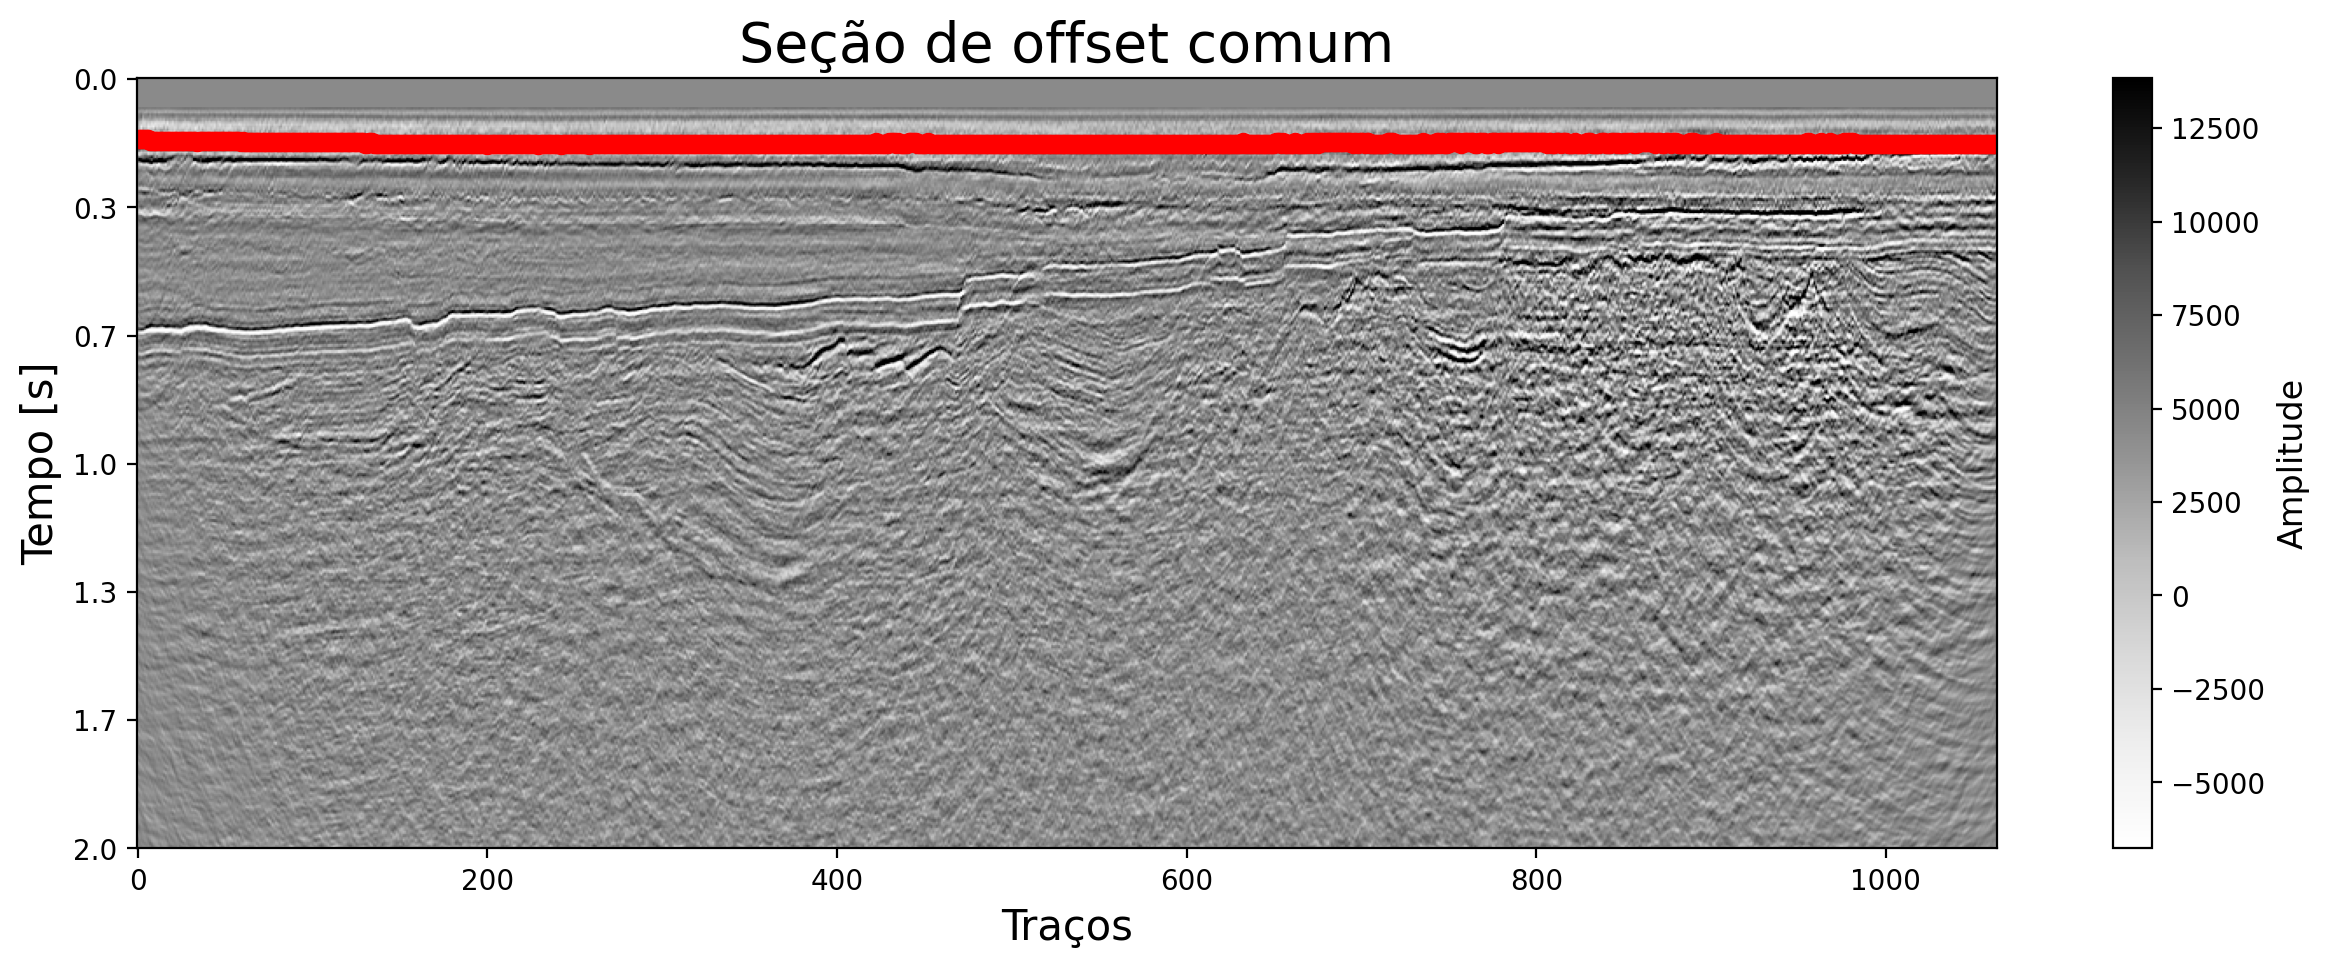
\includegraphics[width=16cm,height=7cm]{../imagens/estimativaWavelet.png}
		\caption{Seção de \textit{offset} comum de menor afastamento com a reflexão do fundo do mar demarcada em vermelho, para ilustrar a janela de tempo efetuada.}
		\label{westim}
	\end{figure}
	
	A figura \ref{inputSource} mostra o resultado da estimativa com seu espectro de amplitudes, juntamente com a fonte sintética baseada no conteúdo de frequência da fonte estimada. O parâmetro de discretização temporal foi de 0,0005 segundos com o total de 3000 amostras no tempo, totalizando 1,5 segundos de simulação. A discretização da fonte é a mesma do tempo de modelagem, pois a fonte está no domínio do tempo contendo 400 amostras.
	\begin{figure}[htp!]
		\centering
		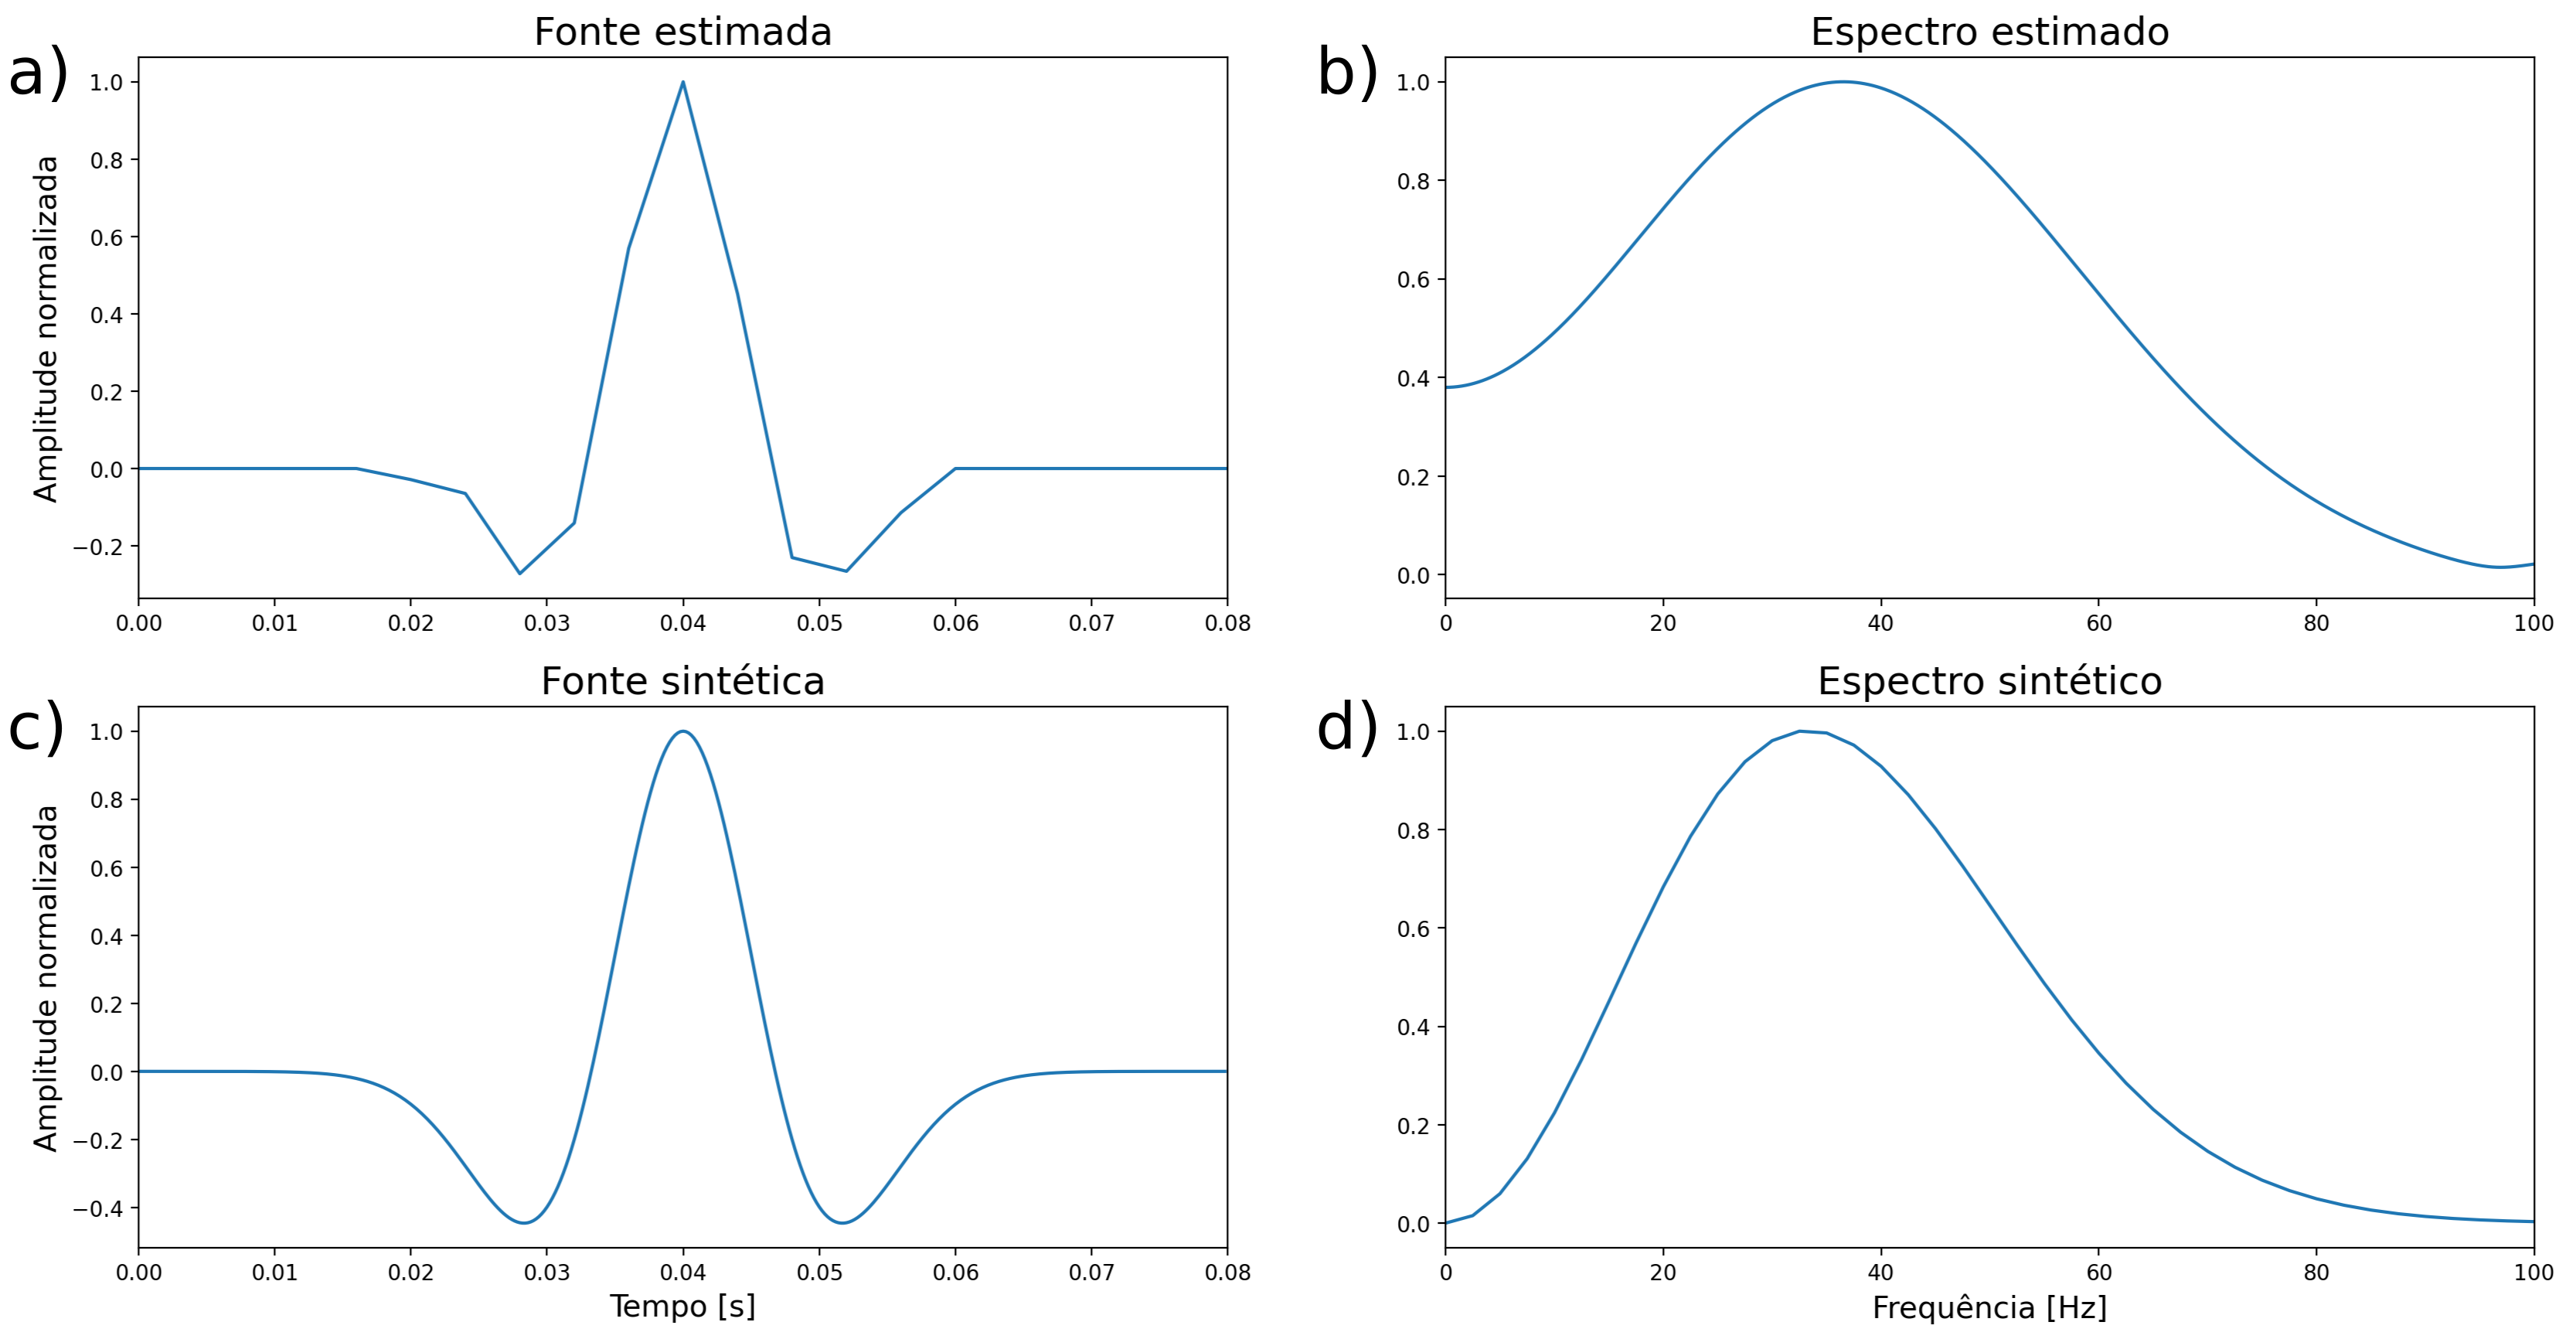
\includegraphics[width=14cm,height=7cm]{../imagens/waveletsModeling.png}
		\caption{Fonte estimada \textbf{a)} com seu respectivo espectro de amplitudes \textbf{b)} e fonte sintética \textbf{c)} baseada na assinatura em frequência da fonte estimada com parâmetro de discretização de 500 $\mu s$ e 400 amostras no total.}
		\label{inputSource}
	\end{figure}
	
	\newpage
	Os procedimentos de pré-aplicação da fonte na modelagem foram realizados como mostrado na figura \ref{wavelets}. A integral numérica, utilizando a técnica discreta da soma corrida, foi aplicada para se obter a integral da Ricker e o filtro, para corrigir a fase, foi aplicado no domínio da frequência com o objetivo de se enxergar uma Ricker no domínio do campo de onda. Todos os procedimentos aplicados na fonte sintética de referência. 	

\section{Pré-condicionamento para o empilhamento do dado sintético}

	Após a modelagem sísmica concluída, o dado gerado necessitou passar por certos condicionamentos antes de refazer o processo de análise de velocidades e empilhamento. A figura \ref{sismicaBruta}, mostra um dos sismograma sintéticos resultantes gerado a partir do algoritmo de simulação sísmica. O efeito a se corrigir, parte do pressuposto que a fonte sintética tem um tempo de injeção que atrasa todo o dado em dimensões da metade do tamanho em amostras da fonte. 

	Para resolver esse atraso no dado, foram removidas as 200 primeiras amostras de todos os sismogramas sintéticos, que não tinham sinal de amplitude pois se referiam à parte anti-causal da fonte sintética. Removendo o atraso e avançando o sismograma no tempo, a parte inferior, ou seja, os tempos finais do dado são considerados como ruídos e foram corrigidos fazendo a substituição do conteúdo de amplitude por um ruído contínuo de $5 \cdot 10^{-6}$. Esse valor se mostrava comum na região antes do silenciamento.   

	\begin{figure}[htp!]
		\centering
		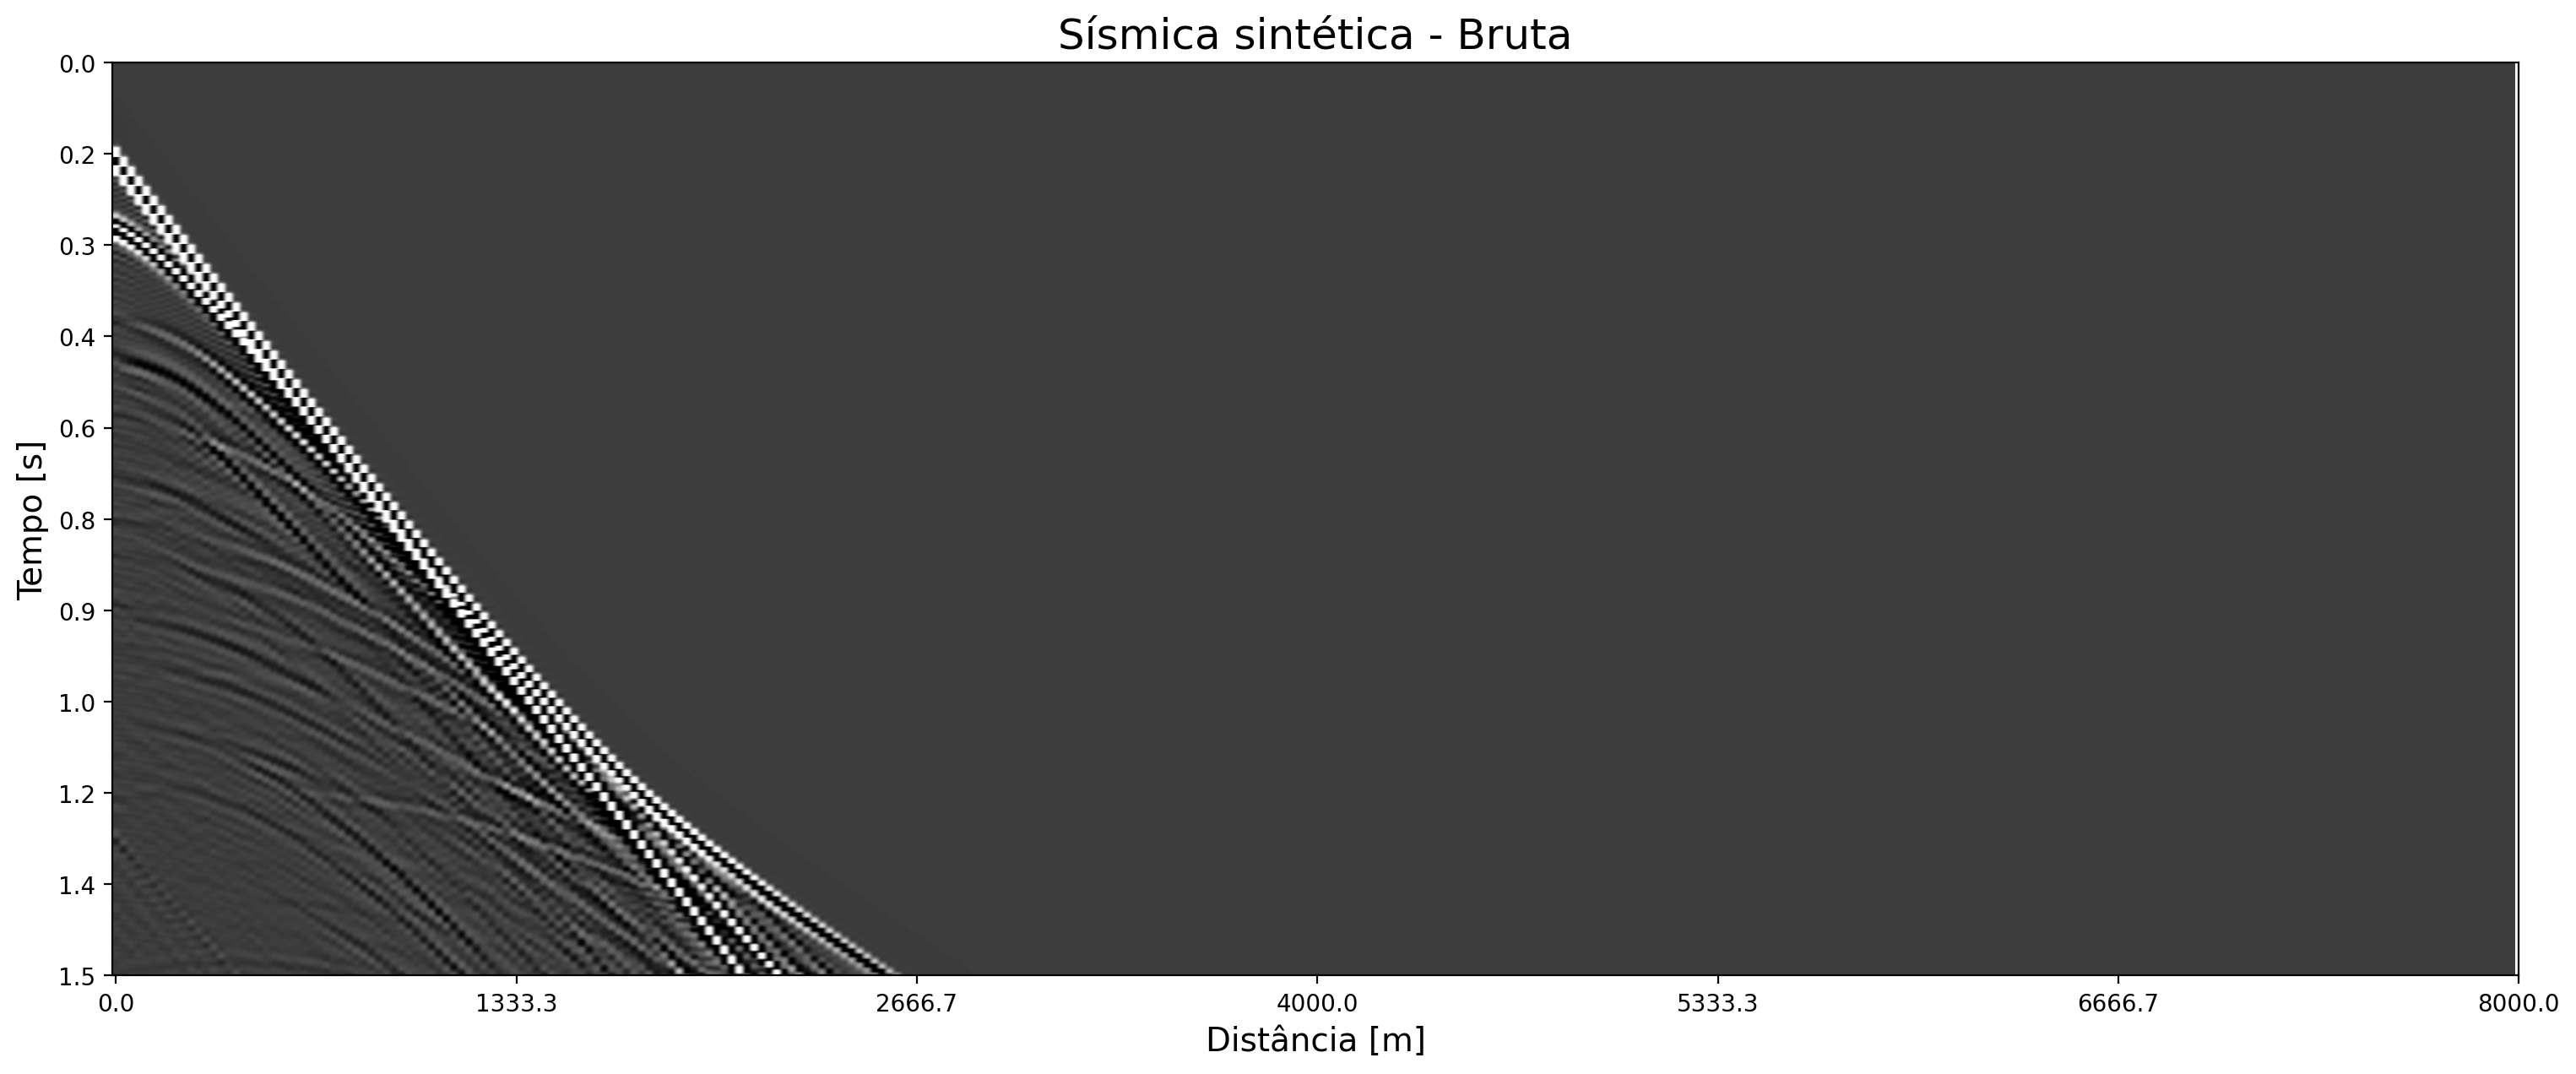
\includegraphics[width=16cm,height=8cm]{../imagens/sismicaSinteticaBruta.png}
		\caption{Sismograma bruto retirado do algoritmo de modelagem sísmica.}
		\label{sismicaBruta}
	\end{figure}

	\newpage
	A figura \ref{sismicaLag}, mostra o avanço do sinal de amplitudes para as amostras superiores evidenciando, em tempos abaixo de 1,4 segundos, as amplitudes ainda atrasadas. O tempo real retirado foi de 0,1 segundos, se baseando na amostragem da aplicação da fonte e no parâmetro de discretização temporal da simulação sísmica.

	\begin{figure}[htp!]
		\centering
		\includegraphics[width=16cm,height=8cm]{../imagens/sismicaLag.png}
		\caption{Avanço de todo o sismograma no tempo para retirar o efeito de aplicação da fonte sintética. Tempos a partir de 1,4 se tornam ruídos e deverão ser corrigidos.}
		\label{sismicaLag}
	\end{figure}

	A última correção nos sismogramas ainda em formato de matriz genérica, ou seja, somente com sinal de amplitude, foi a retirada da onda direta e ondas refratadas dos sismogramas. 
	
	Foi implementado um sistema de silenciamento, onde os parâmetros são dois pontos, inicial e final, para traçar uma reta. A partir desta reta, as amostras à direita de cada sismograma receberam o valor zero, removendo assim a influência da onda direta e das ondas refratadas dos processos posteriormente efetuados como, o de análise de velocidades, correção NMO e empilhamento do dado sintético. A figura \ref{sismicaMute}, mostra o resultado final após as alterações, em um sismograma, realizadas em todos os 1064 sismogramas sintéticos. 		

	Os dados gerados pelo algoritmo de modelagem sísmica são apenas valores de amplitude armazenados em um arquivo no formato binário \textit{float}. Para que os dados sejam lidos pelo pacote \textit{Seismic Unix}, deve-se adicionar o cabeçalho dos dados no formato do \textit{Seismic Unix} (\textit{Header} do dado). O programa usado para fazer o pré-condicionamento do dado sintético adiciona as informações da aquisição em cada traço, utilizando a biblioteca do python chamada \textit{segyio}. Assim, um dado puramente com valores de amplitude, ganha um arquivo de identificação para que o pacote \textit{Seismic Unix} consiga operar a partir das informações que acompanham o dado.
	
	Após a transformação do dado para o formato segy, um comando específico do \textit{Seismic Unix} importa o dado, obtendo um dado em formato su, idêntico ao procedimento realizado com o dado real. 

	\begin{figure}[htp!]
		\centering
		\includegraphics[width=16cm,height=8cm]{../imagens/sismicaMute.png}
		\caption{Sismograma condicionado para realização dos processos de ordenação em CMP, análise de velocidades, correção \textit{normal move out} e empilhamento.}
		\label{sismicaMute}
	\end{figure}
	
	Assim, o dado sintético foi ordenado no domínio do ponto médio comum e os processos de análise de velocidades, correção \textit{normal move out} e empilhamento foram realizados, semelhante aos executados no dado real. No tópico resultados e discussões serão abordadas comparando as seções empilhadas e migradas dos dados real e sintético.   

\chapter{Resultados e discussões}

	O primeiro resultado obtido está ilustrado na figura \ref{comparision}, onde as duas seções, tanto real quanto sintética, são mostradas sem a presença da marcação dos horizontes. Esse resultado apresentou uma diferença significativa na posição em tempo dos horizontes, nitidamente notável. As diferenças apontam uma baixa velocidade presente no modelo de velocidades estimado a partir do dado real, pois as reflexões da seção sintética estão atrasadas no tempo em relação às reflexões do dado empilhado real.

	\begin{figure}[htp!]
		\centering
		\includegraphics[width=16cm,height=10cm]{../imagens/comparision.png}
		\caption{Resultado utilizando a metodologia apresentada. Seção empilhada real \textbf{a)}, gerada a partir das velocidade RMS da análise de velocidades dos sismogramas CMP reais. Seção empilhada sintética \textbf{b)}, gerada a partir da simulação sísmica em meios elásticos isotrópicos, utilizando o modelo de velocidades intervalares convertido a partir do modelo de velocidade RMS dos sismogramas CMP reais. O processos de empilhamento e migração sintéticos utilizaram a própria velocidade RMS dos sismogramas CMP sintéticos.}
		\label{comparision}
	\end{figure}

	Apesar da estimativa do modelo de velocidades não ter sido precisa o suficiente em relação aos valores de velocidade, o modelo apresentou uma estrutura relativamente boa. A partir dessa informação, a seção sintética empilhada apresentou uma correlação estrutural satisfatória em relação aos refletores do dado real, só que atrasada no tempo. A figura \ref{comparisionHrz}, mostra as seções empilhadas com os horizontes, retirados da seção empilhada real, projetados. 

	\begin{figure}[htp!]
		\centering
		\includegraphics[width=16cm,height=10cm]{../imagens/comparisionHRZ.png}
		\caption{Projeção dos horizontes na seção real \textbf{a)} e sintética \textbf{b)}. Os horizontes foram retirados da seção empilhada real e projetados em ambas as seções para comparar as principais diferenças.}
		\label{comparisionHrz}
	\end{figure}

	\newpage
	O primeiro horizonte do dado sintético, abaixo do fundo marinho, está significativamente mal correlacionado com o correspondente no dado real. Sendo que, uma velocidade mal estimada na parte inicial do modelo, prejudica todas as outras reflexões. A diferença pontual para o primeiro horizonte abaixo do fundo marinho é de aproximadamente 0.15 segundos, sendo maior na parte central do modelo de velocidades da onda compressional. 
	
	Além do erro significativo encontrado no primeiro horizonte, a reflexão do fundo marinho possui pequenos erros causados pela má estimativa da profundidade do fundo marinho, coletado da seção empilhada real. Pois a estimativa de profundidade foi feita fixando a velocidade da camada d'água como 1500 metros por segundo. Entretanto foi mantida a velocidade gradual encontrada a partir do processo de análise de velocidades e interpolações.
	
	Para verificar o erro na estimativa, um estudo mais aprofundado da geologia foi realizado. Em \citeonline{ruffell1995seismic}, estão detalhadas as características geológicas do mar Celta em conjunto com o fluxo sedimentar do canal de Bristol. O artigo também mostra seções crono-estratigráficas baseadas em interpretações sísmicas e, como grande valor para a estimativa de velocidades, perfis de poços mostrando a litologia da região do mar Celta (figura \ref{stratigraphy}). Os perfis de poços mostrados em \citeonline{ruffell1995seismic} estão próximos de onde o dado sísmico real foi adquirido.       

	\newpage
	\begin{figure}[htp!]
		\centering
		\includegraphics[width=16cm,height=17cm]{../imagens/pocos.png}
		\caption{Perfis de poços localizados próximos à região de aquisição sísmica, evidenciando uma camada espessa de carbonatos superficiais. Rochas carbonáticas possuem velocidade da onda sísmica compressional superior à rochas clásticas em baixas profundidades (Retirado de \citeonline{ruffell1995seismic}).}
		\label{stratigraphy}
	\end{figure}
%
	Baseado nos perfis de poços, mostrados na figura \ref{stratigraphy}, a estratégia adotada para tentar corrigir os efeitos de atraso em tempo na seção empilhada sintética foi aplicar um gradiente de velocidade decrescente em relação ao tempo. A aplicação foi no domínio do tempo, como mostrado na figura \ref{modificationTime}, para que, posteriormente, uma nova conversão tempo-profundidade seja executada. Para a construção deste novo modelo, o cálculo da profundidade do fundo marinho foi aprimorado, levando em consideração a aproximação das velocidades da camada d'água como 1500 $m/s$, considerando-a homogênea. 
	
	\begin{figure}[htp!]
		\centering
		\includegraphics[width=16cm,height=14.3cm]{../imagens/modificationTime.png}
		\caption{Aplicação do gradiente de velocidade decrescente com as amostras de tempo, ilustrando as diferenças entre os modelos no domínio do tempo.}
		\label{modificationTime}
	\end{figure}
	
	O gradiente de velocidade decrescente com o tempo foi dimensionado com o intuito de não alterar a grandeza geral do modelo de velocidades, mas sim de aumentar a velocidade das camadas iniciais, como mostra a figura \ref{modificationTime}. As primeiras velocidades, antes da transformação, eram em torno de 1700 a 1900 metros por segundo. Com a aplicação se tornaram de 2600 a 2800 metros por segundo, mais condizentes com as rochas carbonáticas superficiais. O gradiente se relaciona com as velocidades da seguinte maneira
%
	\begin{equation}
		grad[i,j] = 1000 - 2,8 \cdot i,
	\end{equation}
%
	\noindent sendo $i$ a direção das linhas e $j$ colunas. Os valores são calculados desde o início da matriz modelo, porém as velocidades geradas acima do horizonte do fundo marinho são desconsideradas. A partir da geração do modelo em tempo, pôde-se realizar uma nova conversão tempo-profundidade, sendo que por consequência da elevação de velocidade, a profundidade do modelo também aumentou. 

	\newpage 	
	A nova profundidade se tornou 2150 metros contendo 323 amostras na vertical, com parâmetro de discretização espacial na faixa de 6,656 metros. A figura \ref{modificationDepth}, mostra a modificação dos modelos convertidos em profundidade, sendo que no modelo corrigido para o carbonato superficial, a velocidade da camada d'água foi homogeneizada com valor de 1500 metros por segundo.  
	
	\begin{figure}[htp!]
		\centering
		\includegraphics[width=16cm,height=16cm]{../imagens/modificationDepth.png}
		\caption{Aplicação do gradiente de velocidade decrescente com o tempo, mostrando os modelos após a conversão tempo-profundidade.}
		\label{modificationDepth}
	\end{figure}
	
	Após a criação do modelo em profundidade e definição do parâmetro de discretização espacial, o modelo abrupto foi gerado, a partir da coleta das velocidades médias do modelo corrigido para os carbonatos superficiais. Sendo assim, a estimativa das novas velocidades cisalhantes e das densidades puderam ser efetuadas, modelos mostrados na figura \ref{modeloInputCorr}, para simular novamente a aquisição sísmica completa com 1064 tiros. 

	\begin{figure}[htp!]
		\centering
		\includegraphics[width=16cm,height=15cm]{../imagens/ModelosInput_Corr.png}
		\caption{Modelos de entrada, adaptados e baseados na geologia regional, para gerar novos resultados na expectativa de ajustar melhor a seção empilhada real adquirida na margem sudoeste da Inglaterra.}
		\label{modeloInputCorr}
	\end{figure}
%	
	A mesma metodologia foi aplicada neste novo pacote de dados sísmicos sintéticos gerados através de modelagem sísmica para meios elásticos isotrópicos. Primeiro, o pré-condicionamento e aplicação do \textit{Header} no dado sísmico sintético, em seguida, ordenação de traços para gerar os sismogramas CMP e realização da análise de velocidades, por fim, a construção da seção empilhada e migrada em tempo. 
	
	O resultado obtido está representado na figura \ref{comparisionCorr}. Com o aumento da velocidade observa-se o aparecimento de múltiplas internas, que são as reverberações da onda entre as camadas. Foi feita a multiplicação de cada traço empilhado por um fator de tempo ao quadrado para elevar as amplitudes em tempos mais longos, uma filtragem bruta do espalhamento geométrico. Com a aplicação do filtro, ruídos também foram amplificados. 
		
	\begin{figure}[htp!]
		\centering
		\includegraphics[width=16cm,height=11cm]{../imagens/comparision1HRZ.png}
		\caption{Comparação das seções empilhadas e migradas após o processo de correção do modelo de velocidades baseado na geologia regional. A nova seção sintética \textbf{b)} aparenta melhor correlação com o dado sísmico empilhado real \textbf{a)}.}
		\label{comparisionCorr}
	\end{figure}
	
	Os horizontes projetados nas seções, mostram nitidamente uma melhora significativa na comparação das reflexões retiradas do dado real em relação aos horizontes sintéticos, após a transformação do modelo de velocidades.
	
	Para inicializar o processo de análise dos resultados, todos os horizontes foram interpretados, agora nas seções sintéticas geradas. Entretanto, somente cinco horizontes estarão presentes na análise. A figura \ref{hrzs}, mostra a disposição dos horizontes que serão analisados, projetados nas seções sísmicas. Os horizontes estão identificados por siglas, sendo hrz0, o horizonte do fundo marinho, hrz1 e hrz2 horizontes iniciais logo abaixo do fundo marinho, hrz5, um horizonte intermediário, e hrz7, o último horizonte interpretado. Esses horizontes foram escolhidos por estarem demarcados inteiramente na seção, sem interrupções. Os horizontes com interrupções, ou seja, os que não possuem a mesma quantidade de amostras que a seção sísmica, sofreram alterações em quantidade de amostra de seção para seção, sendo que essa alteração dificultaria o processo de análise.     

	O processo de análise consiste em verificar o erro absoluto entre os horizontes da seção empilhada, gerada a partir do dado real, em relação aos horizontes das seções geradas a partir dos dados sintéticos. Então, a operação foi feita por amostra de horizonte, extraindo o erro absoluto, em tempo, de cada amostra (Equação \ref{erro}).  
	
	\begin{figure}[htp!]
		\centering
		\includegraphics[width=16cm,height=15cm]{../imagens/interpHrz.png}
		\caption{Seções empilhadas, migradas e devidamente interpretadas em tempo. Ilustração dos horizontes selecionados, da seção real \textbf{a)}, sintética inicial \textbf{b)} e sintética corrigida \textbf{c)}, para a realização das análises de erro.}
		\label{hrzs}
	\end{figure}

	A figura \ref{analise}, mostra os histogramas gerados para todos os horizontes interpretados, sendo que os traços com indicador "Bruto", correspondem à diferença entre os horizontes extraídos da seção empilhada real em relação ao extraído da seção sintética sem correção. Os traços com indicador "Corrig.", correspondem à diferença entre o horizonte real em relação ao sintético corrigido. As amplitudes dos histogramas representam a quantidade de amostras por horizonte que possui um erro associado de tempo, sendo que na figura \ref{analise}, as amplitudes estão normalizadas.    

	O caso ideal para os histogramas seria um traço com amplitude 1 no tempo zero e valores nulos para os demais tempos, significando que os horizontes não possuem diferenças entre si. A equação que melhor representa a metodologia de análise tem o formato
%	
	\begin{equation}
		e_{abs}(hrz_i) = ABS(hrz_i^{obs} - hrz_i^{cal}),
		\label{erro}
	\end{equation}
%	   
	\noindent sendo o erro absoluto para cada horizonte $e_{abs}(hrz_i)$ o módulo da subtração entre o horizonte $hrz_i^{obs}$ retirado da seção real com o horizonte $hrz_i^{cal}$ coletado da seção sintética.
	
	Então, a melhor forma de se analisar a figura \ref{analise} seria observar as distribuições de erro tendendo à zero, pois quanto mais valores de erro próximos de zero, mais precisa foi a estimativa do modelo e consequentemente, melhor os horizontes se ajustaram. 

	\begin{figure}[htp!]
		\centering
		\includegraphics[width=14cm,height=14cm]{../imagens/analise.png}
		\caption{Histogramas gerados a partir do erro absoluto dos horizontes analisados com amplitude normalizada. Traços com identificador "Bruto", foram gerados a partir das diferenças absolutas entre horizonte real e sintético sem modificação no modelo. Agora, os traços identificados como "Corrig.", foram gerados a partir das diferenças entre o horizonte real e sintético com modelo corrigido.}
		\label{analise}
	\end{figure}

	Observando as curvas na figura \ref{analise}, a constatação da melhoria no modelo de velocidades, gerado a partir da aplicação do gradiente decrescente com o tempo, se concretiza. A modificação mostrou melhorias até mesmo no horizonte do fundo marinho, hrz0, por consequência da construção mais precisa das velocidades sísmicas da onda compressional na camada d'água. De maneira geral, o erro absoluto presente nos horizontes diminuiu consideravelmente após a modificação do modelo de velocidades. O modelo ainda pode ser melhor aperfeiçoado, porém, métodos mais robustos de inversão sísmica para a obtenção de propriedades do meio devem ser aplicados.  

	Para elucidar o trabalho, a figura \ref{fluxograma}, mostra a organização dos processos executados por etapa até concluir com a análise dos resultados. 

	\begin{figure}[htp!]
		\centering
		\includegraphics[width=16cm,height=11.5cm]{../imagens/fluxograma.png}
		\caption{Fluxograma completo das etapas discutidas neste trabalho. Três fluxos principais, o primeiro até gerar a seção real migrada, e os outros dois gerando seções sintéticas para serem comparadas e analisadas.}
		\label{fluxograma}
	\end{figure}

	Então, a partir de um pacote de dados sísmicos, foram gerados três seções empilhadas, sendo a primeira resultante da análise do próprio dado real. A segunda, foi gerada por consequência da construção do modelo de velocidades e modelagem sísmica em meios elásticos isotrópicos, e a terceira seção, foi gerada a partir da modelagem sísmica utilizando o modelo corrigido. As três seções resultaram de processos semelhantes, sendo que cada dado recebeu uma estima de velocidade RMS única para realizar o empilhamento e migração em tempo. Os resultados foram baseados na interpretação e comparação dos horizontes entre as seções geradas, verificando as diferenças absolutas entre eles. 

\chapter{Conclusão}

	O método da análise de velocidades não identificou a anomalia rasa de alta velocidade identificada devido ao \textit{chalk} relatado nas bibliografias. Todavia, os contrastes de velocidade foram coerentes ao ponto de gerar estruturas compatíveis na parte mais profunda  do modelo de velocidades compressionais resultante. A atualização realizada no modelo de propriedades foi exclusivamente ligada à geologia, observando a presença, em perfis de poços, das rochas carbonáticas superficiais. O gradiente de velocidade decrescente com a profundidade foi aplicado pelo contexto geológico observado nas referências bibliográficas, sendo constituído por camadas plano-paralelas horizontais em uma região com limite tectônico distensivo.           
	
	Com base nos resultados, nota-se uma boa aplicabilidade do método de análise de velocidades para estimativa inicial do campo de velocidades da onda P, que apesar de ter limitações, ainda pode ser aplicado em regiões geologicamente simples. Observa-se também que, para contextos geológicos estratigraficamente plano-paralelos, gradientes de velocidade corrigem bem o modelo, sendo que muitas vezes os gradientes são usado para gerar um modelo de velocidades inicial em esquemas de inversão sísmica, como por exemplo a tomografia.
	
	Um próximo passo seria investir na projeção dos dados sísmicos em profundidade, ou seja, aplicar um processo de migração em profundidade utilizando a aproximação acústica do meio, por estratégias como traçado de raios ou a extrapolação do campo de onda. Outro passo que pode ser explorado, seria a aplicação de um processo de inversão tomográfica para obtenção de melhorias pontuais no modelo de velocidade da onda compressional e assim, melhorar o resultado do processo de migração em profundidade.    

\postextual

% Referencias bibliográficas
\bibliography{referencias}

% Apêndices
\begin{apendicesenv}

    % Imprime uma página indicando o início dos apêndices
    \partapendices

	\chapter{Propagação da onda 2D}
	
	Será apresentada a função, escrita em linguagem C, que resolve numericamente a equação \ref{elasticWave} por diferenças finitas com operadores de segunda ordem no tempo e espaço. Nota-se a presença de dois laços de repetição principais, o primeiro resolve as tensões \textit{Txx}, \textit{Tzz} e \textit{Txz}, e o segundo resolve as velocidades de partícula \textit{Vx} e \textit{Vz}. Os parâmetros elásticos de densidade, compressibilidade e cisalhamento são representados por \textit{rho}, \textit{L} e \textit{M} respectivamente. Os campos de onda e modelos elásticos 2D são representados por \textit{arrays} 1D com dimensões espaciais de \textit{nxx} delimitando a distância e \textit{nzz} a profundidade. O algoritmo segue no formato  
	\newline	
		
	\lstinputlisting[language=C, basicstyle=\tiny,
	keywordstyle=\color{blue}, stringstyle=\color{green},
	commentstyle=\color{green}, extendedchars=true,
	showspaces=false, showstringspaces=false,
	numbers=left, numberstyle=\tiny,
	breaklines=false]{../codes/elasticIsotropicStressStencil2D.h}
	
\end{apendicesenv}

%% Anexos
%\begin{anexosenv}
%
%    % Imprime uma página indicando o início dos anexos
%    \partanexos
%
%\end{anexosenv}

\phantompart
\printindex

\end{document}